% This sample file is dedicated to the public domain.
\documentclass[12pt]{myucthesis}

%\nofiles
% The above command prevents latex from writing its auxiliary
% files. This is useful if you want to manually tweak them before you
% generate your final PDF.


% Page layout. The fancyhdr package may complain about the need for a
% larger headheight, depending on how long chapter titles are; if left
% unspecified in the geometry setup, it defaults to 12pt. The
% "showframe" option causes the geometry package (version >= 5.0) to
% show a frame around the margins on every page, which is great for
% checking that you don't overflow anywhere.

%\usepackage[letterpaper,includehead,margin=1in,headheight=15pt,showframe]{geometry}
\usepackage[papersize={8.25in, 10.75in},includehead,margin=0.875in,headheight=30pt]{geometry}
\usepackage{fancyhdr}
\pagestyle{fancyplain}
\lhead[\fancyplain{\thepage}{\thepage}]{\fancyplain{}{\scshape\rightmark}}
\rhead[\fancyplain{}{\scshape\leftmark}]{\fancyplain{\thepage}{\thepage}}
\chead{}
\cfoot{}
\lfoot{}
\rfoot{}


% Bibliography stuff:

\newcommand{\newblock}{\par} % need this for some natbib internal bug
\bibliographystyle{naturemag}
\bibstyle{naturemag}
\def\bibpreamble{\addcontentsline{toc}{chapter}{Bibliography}} % get a good TOC entry


% Other setup:

\usepackage[T1]{fontenc} % see http://tinyurl.com/67zdxwf
%\usepackage[colorlinks,urlcolor=blue,citecolor=blue,linkcolor=blue,pdfusetitle]{hyperref}
\usepackage[colorlinks,urlcolor=black,citecolor=black,linkcolor=black,pdfusetitle]{hyperref}   %Use this instead of above to make links black.  
\usepackage{pdflscape} % allows landscape-oriented figures with PDF page rotation
\usepackage{aasmacros,amsmath,amssymb,graphicx}
\usepackage{mydeluxetable} % deluxetable customized to play well with ucthesis

%boldface vectors for the nonlinear optics section
\renewcommand{\vec}[1]{\mathbf{#1}}

%useful QM stuff
\def\bra#1{\langle#1|}
\def\ket#1{|#1\rangle}
\def\xpec#1{\langle#1\rangle}

%easier equation references
\def\eqref#1{(\ref{#1})}


\begin{document}
\ssp % single spacing
\hypersetup{pageanchor=false}
\title{Quantum Feedback and Traveling-wave Parametric Amplification in Superconducting Circuits}
\author{Christopher Stewart Macklin} % must match BearFacts!
\degreesemester{Spring}
\degreeyear{2015}
\degree{Doctor of Philosophy}
\numberofmembers{3}
\chair{Irfan Siddiqi}
\othermembers{
John Clarke \\
K B Whaley
}
\field{Physics}
\campus{Berkeley}

\maketitle
\copyrightpage

\begin{abstract}
Feedback control in classical systems is an indispensable, ubiquitous tool.  The theoretical basis for achieving optimal classical control is well understood, and crucially relies on a very classical assumption: that measurements of the state of a system under control need not perturb that state.  In a quantum context this assumption is fundamentally invalid.  Although many aspects of the theory of quantum feedback control are relatively well developed, the technological basis for feedback control of a single quantum system has only very recently matured.  We demonstrate the experimental realization of a quantum feedback control protocol, perpetually stabilizing the coherent Rabi oscillations of a superconducting qubit.  This is the first utilization of quantum feedback control for stabilizing a dynamical process, and the first application of quantum feedback in a solid-state system of any kind.  This demonstration comprises the first half of this thesis.  The feedback protocol is predicated on the ability to make high-fidelity quantum measurements, which are enabled by quantum-limited Josephson parametric amplifiers (JPAs).  The design and realization of the novel Josephson traveling-wave parametric amplifier (JTWPA) comprises the second half of this thesis.  The JTWPA achieves order-of-magnitude improvements over state of the art JPAs in bandwidth and signal power handling while providing quantum-limited noise performance, potentially enabling the simultaneous readout of dozens of superconducting qubits and the generation of broadband multi-mode squeezing in the microwave domain.
\end{abstract}

\hypersetup{pageanchor=true}
\begin{frontmatter}

\begin{dedication}
\null\vfil
{\large
\begin{center}
DEDICATED TO ALL THE CATS!
\end{center}}
\null\vfil
\end{dedication}

\tableofcontents
\listoffigures % optional
%\listoftables % optional

% If using code.sty, can also add:
%% \listofcodes
%% \addcontentsline{toc}{chapter}{List of Code Examples}

\begin{acknowledgements}

I acknowledge the support and contributions of an uncountable number of people.  What follows is a profoundly incomplete list, ordered roughly chronologically.
\paragraph{}
\textbf{Diane, Allen, and Kate}, my biological family: I couldn't have done it (everything) without you.  Dad, I wish you had been able to live to see this day, and I hope you knew what a profound influence your scientific career had on the course of my life.
\paragraph{}
\textbf{Dr. Richard Piccioni}, my high school physics teacher: every day of your class I felt my understanding of the world deepen, and your enthusiasm, passion, and patience have inspired me to this day.  I have absolutely no idea what I would be doing with my life now if you hadn't guided me towards studying physics.
\paragraph{}
\textbf{Prof. Ritchie Patterson}, my first undergraduate research advisor at Cornell: your support and guidance were essential in my development as a self-confident researcher, and I am also indebted to you for the time I spent working as part of the CMS collaboration---a key experience which convinced me that I didn't actually want to study particle physics.
\paragraph{}
\textbf{Prof. Keith Schwab}, my final undergraduate research advisor at Cornell: your influence and support were invaluable in shaping my trajectory and my thoughts on physics itself.  My confidence as a young researcher was far greater after the time I spent in your lab.  I cannot thank you enough for introducing me to quantum measurement science.
\paragraph{}
\textbf{Prof. Irfan Siddiqi}, my graduate research advisor: you've said many times that the lab doesn't have your name on the door, and this atmosphere of empowerment and shared responsibility has created a superb environment for growth and learning.  The transparency with which you manage the lab is highly beneficial to the students and postdocs, providing us with insight into the hardest part of science: the byzantine, political, messy process of acquiring and maintaining funding.
\paragraph{}
\textbf{Dr. Ofer Naaman}, my first postdoc mentor at QNL: your tough love got me off to a good start in the lab, and my long-run scientific productivity was enhanced by learning from your working style.  It has been my great pleasure to shepherd the JTWPA from your original idea to a practical device.
\paragraph{}
\textbf{Dr. Daniel Slichter}: I learned a great deal about conducting science from your working style, especially the tricky process of sussing out just what's happening with a setup which is producing nonsensical results.  Your uncanny ability to summon forth a small laundry list of things to check demonstrated a deep understanding of the technical details of an experiment that still inspires me.  I am also indebted to you for your early experimental work on the JTWPA and your overall guidance.
\paragraph{}
\textbf{Dr. R. Vijay}, my primary postdoc mentor at QNL: I admire your enthusiasm for physics and your willingness to dive all the way deep into an experiment.  Your combination style of getting things working fast with a longer period of perfectionism lead to truly beautiful science.  Working on the quantum feedback experiment with you was an incredible learning experience.  I also thank you for your feedback on this manuscript.
\paragraph{}
\textbf{Dr. Kater Murch}, the ultimate inspiration to stop thinking and start doing right now: I can only aspire to move as fast as you do.
\paragraph{}
\textbf{Prof. Alexander Korotkov}, the theoretical backbone of the quantum feedback project: it was an honor to experimentally realize such a beautiful and simple piece of physics theory, even if quantum mechanics is trivial.  A very good collaboration indeed.
\paragraph{}
\textbf{Kevin O'Brien}: your theoretical work on the JTWPA made this device a practical reality.  I cannot thank you enough for your above-and-beyond efforts in understanding this fascinating device and for being a fabulous collaborator.
\paragraph{}
\textbf{Prof. Will Oliver, Dr. David Hover, and the rest of the MIT-LL team}: thank you for such a productive collaboration to fabricate and realize the JTWPA.  Your expertise brought this device to life.
\paragraph{}
\textbf{Mollie Schwartz}: my excitement at finally having a graduate student minion quickly gave way to awe as you rapidly learned and took over the entire entanglement-by-measurement experiment.  Your mastery of qubit measurements and your well-calibrated measurement setup were essential to acquiring the exquisite data on the noise performance of the JTWPA.  I also thank you for your feedback on this manuscript.
\paragraph{}
\textbf{Dr. Allison Dove, Dr. Emmanuel Flurin, Andrew Eddins, Dr. Shay Hacohen-Gourgy, and Vinay Ramasesh}: thank you for your feedback on this manuscript.
\paragraph{}
\textbf{Prof. John Clarke and Prof. Birgitta Whaley}, my dissertation committee: thank you for your comments, guidance, and of course, your signatures.
\paragraph{}
\textbf{Every member of QNL, past and present}: you made this lab what it is today, and I cannot thank every one of you enough.  The experiments in this dissertation would not have been possible without your technical expertise and communal support.
\paragraph{}
\textbf{The staff at House of Curries}: QNL would have starved long ago without you.
\paragraph{}
\textbf{Little Cat and Future Cat}, my furriest friends and informal QNL mascots: your images grace every computer in the lab.
\paragraph{}
\textbf{Elizabeth}, my love and companion: I can't imagine a life without you.

\end{acknowledgements}
\end{frontmatter}

\chapter{Introduction}
\label{c:intro}

Over the past several decades, the technology available for performing quantum physics experiments has advanced to a point where isolating, controlling, and measuring individual quantum degrees of freedom has become routine.  Early in this process, much attention was focused on creating techniques aimed at harnessing ``naturally-occurring'' quantum systems into this regime.  For example, precision measurement and manipulation of single electronic state transitions in the spectra of individual highly excited or ionized atoms has resulted in the direct observation of a number of fundamental quantum effects in experiments with a high degree of conceptual simplicity and beauty\footnote{The experimental apparatuses themselves, however, are of course far from simple.} \cite{PhysRevLett.65.976,PhysRevLett.72.3339,Nogues1999,Monroe24051996,Myatt2000,RevModPhys.73.565}, and were the subject of the 2012 Nobel prize in physics \cite{Nobelprize.org2012}.  More recently, the type and variety of natural quantum systems which can be manipulated at the single degree of freedom level have proliferated, including cold atomic gasses trapped in optical lattices \cite{Bloch2005}, single spins in diamond \cite{ISI:000321694300003}, the nuclear and electronic spins of a single phosphorous donor in silicon \cite{Pla2012}, and the spin and charge degrees of freedom of a single electron trapped in a quantum dot \cite{ISI:000321694300004} (this list is not exhaustive).

While these systems may not all be exactly ``natural'', per se, the quantum degrees of freedom are all fundamentally microscopic: single electron orbitals, the spins of single atoms or electrons, or the motional degree of freedom of a single atom.  Remarkably, there now exist classes of coherent systems whose quantum degrees of freedom are macroscopic quantities that have been specially \textit{engineered} to express quantum behavior.  In these systems, the collective motion of a very large number of constituent particles constitute a single quantum variable, with all of the same resulting richness and perplexing implications of the quantum systems created by nature.  Unlike natural systems, however, these engineered quantum systems can re-arranged, twisted into different shapes, mutated, and moved into obscure and interesting nooks of their parameter spaces, in some cases permitting the observation of quantum phenomena which are difficult or impossible to observe in hitherto explored systems.

\section{Superconducting qubits and circuit quantum electrodynamics}

A rigorous proposition for searching for quantum-coherent behavior in a macroscopic object came from Leggett in 1980 \cite{1980PThPS..69...80L}; in this paper, he presciently observed that superconducting circuits were the most promising platform then known for observing such behavior.  Indeed, macroscopic quantum tunneling was observed in the phase difference across a current-biased Josephson junction at UC Berkeley in 1987 \cite{PhysRevB.35.4682}.  This experiment set the stage for the full consideration of the currents and voltages in superconducting circuits as quantum degrees of freedom, eventually leading to the first observation of a coherent macroscopic superposition state in a superconducting circuit called a Cooper pair box at NEC in 1999 \cite{Nakamura1999}---the first demonstration of a \textit{superconducting quantum bit (qubit)}.  This first device only maintained quantum coherence over a timescale of about 1 ns.  Sixteen years later, as of the writing of this thesis, superconducting qubits routinely achieve coherence times of tens of microseconds \cite{Paik_3DT,Chang2013}, an improvement of more than four orders of magnitude, and there is still no generally agreed-upon fundamental upper limit to these coherence times.

Superconducting qubits came into their own as a platform for testing quantum theory, especially quantum measurement and feedback control, with the marriage of cavity quantum electrodynamics \cite{RevModPhys.73.565} and superconducting circuits, resulting in the new paradigm of \textit{circuit QED} (or \textit{cQED}) in pioneering experiments at Yale \cite{cQEDtheory,Wallraff2004}.  The cQED architecture can provide controllable strong coupling between a single microwave-frequency photon and a superconducting qubit, as well as ideal, non-destructive measurement of the quantum state of the qubit \cite{Vijay:2011kx,slichterthesis} or the photon state of the cavity \cite{Schuster2007}.  These properties permit, for example, the controlled generation of exotic quantum optical states \cite{Hofheinz2009,Vlastakis2013}, the monitoring and reconstruction of the quantum trajectory of a qubit undergoing continuous measurement \cite{murch_observing_2013,Weber2014,Weber2014a}, and the first observation of the enhancement of an atomic lifetime using squeezed light \cite{murch_reduction_2013}.  The experiment which is the subject of the first half of this thesis, the implementation of a quantum feedback control protocol, crucially relies on the exquisite quantum measurement capability provided by cQED.

Besides their applicability to the study of quantum mechanics, superconducting qubits and cQED have emerged as a viable platform on which to implement fault-tolerant quantum computing protocols \cite{Nielsen2000}, such as the ``surface code'' protocol \cite{PhysRevA.86.032324}.  In the last two years, error rates in multi-qubit devices have approached the minimum threshold necessary to implement the surface code error correction procedures \cite{Barends2014,Riste2014,Chow2014}.  Many technological challenges remain between these proof-of-principle experiments and a viable quantum computer.  At present, high-quality qubit state measurement---essential for the surface code---is performed in these systems with the aid of ultra-low-noise microwave amplifiers based on Josephson junctions \cite{Castellanos-Beltran2008,JPCNature,Hatridge:2011zr}.  The performance of these amplifiers is one of many obstacles which stand in the way of realizing a large-scale quantum computer based on superconducting qubits \cite{Mutus2014,Kelly2015}; the device which constitutes the subject of the second half of this thesis directly addresses this need.

\section{Quantum feedback control}

Feedback control schemes are ubiquitous in classical systems for stabilizing the state of that system against disturbances.  Thermostats, anti-lock brakes, pacemakers, and aircraft flight control systems all utilize the outcome of a measurement to automatically and autonomously steer a system towards a desired state, and hold it there even in the presence of fluctuations.  The operation of these feedback protocols is predicated on the idea that making a measurement of the state of the system need not alter that state.  Of course, if we apply feedback control to a quantum system, this predicate no longer holds: measurements in quantum mechanics are fundamentally invasive \cite{qmcontrol_book}. Thus, quantum feedback control is faced with an additional fundamental challenge: how can we hope to stabilize the state of a quantum system using feedback control if our very measurement of that state disturbs it?

As in many areas of physics, theoretical development in the field of quantum control has significantly outpaced experimental demonstration.  This is in large part due to the technological challenges associated with realizing controllable quantum systems discussed so far in this chapter.  Furthermore, in order to address the question at the end of the previous paragraph, we require not just a controllable quantum system, but one which is capable of realizing a \textit{nearly-ideal, minimally-invasive, continuous quantum measurement}.  The textbook picture of the quantum measurement process involves the instantaneous projection of the quantum system into one of its eigenstates; if we desire to utilize a feedback protocol to stabilize, say, a superposition state of that system, then such a projective measurement is in a sense maximally invasive.  We require, instead, a measurement platform where we can slow down the time scale associated with projecting the system into an eigenstate, until the measurement is slower than the time scale over which feedback occurrs.  Then, we can use our knowledge of the measurement outcome and the action of the feedback loop to \textit{undo the back-action of the measurement} as well as correct for the effect of external disturbances on the system.

The first demonstration of closed-loop feedback control of a single quantum system was implemented by the cavity QED team at ENS in 2011 \cite{haroche_fb}.  In this beautiful experiment, the photon number state of a microwave cavity is weakly probed by a stream of atoms prepared in highly excited Rydberg states. Each atom makes a very weak, non-destructive measurement of the photon number, such that about 50-100 atoms must be detected to fully determine it.  Using a complex Bayesian model, a real-time computer applies a classical control correction to the cavity field after the detection of each atom, with the target of stabilizing the cavity into a particular highly-nonclassical definite photon number state (aka a Fock state).  The action of the feedback control quickly projects the cavity into the desired Fock state with high fidelity, and successfully stabilizes this state in the presence of decoherence associated with the cavity decay lifetime.

Circuit QED provides another path towards realizing a faithful, weak quantum measurement: the continuous weak measurement of the state of the qubit by the small phase shift it induces in the photon field in the cavity \cite{Boissonneault2009,koro11,Girvin2014}.  By measuring the field escaping from the cavity, a continuous tracking of the qubit state is possible, provided that all of the information carried by this field is faithfully recovered by the experimental apparatus.  The experiment which comprises the first half of the results in this thesis leverages this continuous, weak measurement of the qubit state to perform a feedback stabilization of the coherent Rabi oscillations of a superconducting qubit.  The feedback protocol not only corrects for external decoherence of the qubit, but also self-corrects the stochastic back-action of the measurement process itself.

The power carried by the microwave field which conveys qubit state information away from the cavity is extremely small, on the order of a few femtowatts. In contrast, the electronics used to process this signal at room temperature typically expect milliwatts.  As such, to realize this experiment, we require an ultra-low-noise preamplifier which is itself governed by (and ideally limited by) quantum mechanics.

\section{Josephson parametric amplifiers}

In order to realize an amplifier whose performance is limited by quantum mechanics, we turn to the class of devices known as \textit{parametric amplifiers}.  The operating principle of a parametric amplifier is based on the harmonic modulation of a parameter of a nonlinear dynamical system by a strong drive called the \textit{pump}.  The nonlinear element in the system provides one or more terms in the dynamical equation which couple energy between oscillations at different frequencies; thus, when arranged correctly, a small initial signal oscillation grows over time through the nonlinear interaction with the pump, realizing gain.  The mechanism of parametric amplification does not necessarily mandate any energy dissipation; a lack of dissipation also implies a lack of additional fluctuations, implying that parametric amplifiers have the potential to realize quantum-limited noise performance \cite{clerk_revmod}.

The Josephson tunnel junction is a circuit element unique to superconducting circuits which is both highly nonlinear and non-dissipative.  Parametric amplifiers utilizing the Josephson nonlinearity were first demonstrated in 1975 \cite{Feldman1975}, and development continued through the 80s and 90s \cite{1060904,1063665,Yurke1989,Yurke:1996ys}, though the quantum limit proved elusive and these devices did not see much practical use.  More recently, the promising applications of superconducting devices in the fields of quantum measurement and quantum information reignited interest in this type of amplifier, and improved designs have demonstrated robustly quantum-limited noise performance with high gain and sufficient bandwidth for many applications \cite{Castellanos-Beltran2008,JPCNature,Hatridge:2011zr}.

These Josephson parametric amplifiers (JPAs) have been integral to realizing high-quality measurements of superconducting qubits and have enabled many of the groundbreaking experiments mentioned so far in this chapter.  The development of this type of amplifier has been a central activity at the Quantum Nanoelectronics Laboratory (QNL) at UC Berkeley, where the experiments described in this thesis took place.  Improvements in JPA design at QNL have led to the observation of quantum jumps in a superconducting qubit \cite{Vijay:2011kx,slichterthesis}, the demonstration of high-fidelity qubit readout and heralded state preparation \cite{fluxqb}, the observation and statistical analysis of quantum trajectories \cite{murch_observing_2013,Weber2014,Weber2014a}, and the demonstration of measurement-induced entanglement generation between remote qubits \cite{Roch2014}.

The circuit topology for essentially all JPAs involves embedding one or more junctions in some kind of resonant circuit, consisting of one or more distributed-element transmission line resonators or lumped-element LC resonators, with the nonlinear Josephson inductance contributing some fraction of the total inductance.  Although a variety of design improvements have expanded the performance of these devices, the resonant topology fundamentally introduces a limitation called the \textit{gain-bandwidth product}: the product of the gain in amplitude units and the bandwidth is limited to a constant, typically 10 MHz to 1 GHz or so.  As such, essentially all JPAs with amplitude gain of 10 are limited to bandwidths on the order of 1-100 MHz, with most devices achieving about 10 MHz.  Furthermore, the dynamics of the nonlinear resonator restrict how much power can be used to pump the devices, which limits the amount of signal power a JPA can faithfully amplify.

For many experiments this performance is sufficient; however, for the construction of a large-scale quantum computer based on superconducting circuits, it would be desirable to have an amplifier with a much larger bandwidth, which is capable of handling multiple input signals simultaneously, while still retaining quantum-limited noise performance.  The design and realization of a JPA based on a fundamentally different circuit topology---a nonlinear transmission line, rather than a nonlinear resonator---comprises the second half of the results described in this thesis.  The resulting device, dubbed the Josephson traveling-wave parametric amplifier (JTWPA), is not saddled with the same fundamental limitations as a resonator-based JPA.  The JTWPA is able to achieve large gain over gigahertz-scale bandwidths, faithfully amplifying signal powers an order of magnitude larger than the best JPAs yet demonstrated, while achieving nearly quantum-limited noise performance.

\section{Thesis overview}

I begin chapter \ref{c:qm} with the aim of providing an intuitive picture of how quantum limits on measurement arise by discussing two classic thought experiments.  Most of the remainder of the chapter is dedicated to the description of various classes of quantum measurements, focusing on those most relevant to the experiments performed in this thesis, including a brief description of the quantum Bayesian approach to quantum measurement.  I conclude the chapter with a discussion of the theory of the quantum control protocol implemented in the Rabi stabilization experiment, including the analytical derivation of the performance of the feedback loop.

In chapter \ref{c:scqb}, I give an overview of how to construct a qubit from superconducting circuits.  Rather than following the historical approach of starting with the Cooper pair box, I take an alternative approach which I find more intuitive: because modern superconducting qubits are essentially weakly-anharmonic oscillators, I start with a general discussion of anharmonic oscillators and then describe how such a device can be realized using superconducting circuit elements.  Finally, I introduce the basics of cavity QED and the circuit QED implementation, specifically addressing the parameter regime applicable to weak quantum measurement.  Chapter \ref{c:paramps} is the third and final chapter of background material, comprising a discussion of quantum-limited amplifers.  I begin the chapter with a general discussion of the origin of quantum limits on amplification, followed by a description of JPAs, their performance, and the limitations to their performance.  These limitations lead naturally to a brief discussion of traveling-wave amplifiers and the JTWPA as an alternative to the traditional JPA.

Chapters \ref{c:qfb} and \ref{c:qfb_results} comprise the experimental realization of the stabilization of Rabi oscillations using quantum feedback control.  In chapter \ref{c:qfb}, I provide a thorough description of the experimental apparatus, including a variety of important calibration and tuning experiments necessary to demonstrate high-quality feedback and interpret the results.  Chapter \ref{c:qfb_results} is entirely dedicated to the experimental results attained in the quantum feedback experiment, including frequency- and time-domain measurements of the stabilized state as well as tomographic state reconstruction and validation.  In addition to the results directly pertaining to feedback stabilization of Rabi oscillations, this chapter includes a beautiful piece of unpublished data related to variable-strength continuous quantum measurement.

Chapters \ref{c:twpa_theory} and \ref{c:twpa_exp} comprise the theory and experimental results for the JTWPA, respectively.  In chapter \ref{c:twpa_theory}, I provide some background on nonlinear optics, as the theory of the JTWPA is partially derived from it.  I continue with a presentation of the derivation of the continuum wave equation (the key link between the circuit-theory description of the JTWPA and the nonlinear-optical description) and the requirements for realizing efficient parametric amplification.  Next, I discuss the derivation of the dispersion relation of the JTWPA and the associated ``resonant phase matching'' dispersion-engineering technique we created to satisfy the crucial nonlinear optical phase matching criterion needed for efficient amplification.  I close the chapter with a detailed presentation of the theoretical performance predicted for a practical device.

In chapter \ref{c:twpa_exp}, I describe a precise experimental assessment of a JTWPA device, validating the theory presented in chapter \ref{c:twpa_theory}.  The amplifier calibration experiments utilize a cQED system in the weak measurement limit to enable high-precision noise measurements.  I conclude the chapter with a discussion of the performance of the JTWPA in a projective qubit measurement, and extrapolate those results to show that it could serve as the low-noise preamplifier for the simultaneous readout of as many as 20 superconducting qubits.  I close the thesis with some future directions in quantum feedback control and JTWPA development in chapter \ref{c:conclusion}.

\section{Summary of key results}

The quantum feedback experiment presented in this thesis is the first realization of a quantum feedback control protocol in a solid-state system, and also the first demonstration of a quantum feedback protocol for stabilizing a dynamical quantum state.  The protocol stabilizes the target state with an efficiency of about 45\%, in excellent agreement with the predictions from theory when the imperfections in the experiment are accounted for.  As such, this experiment constitutes a validation of a significant body of quantum feedback control theory.  To quote Howard Wiseman in his \textit{Nature} News \& Views article on the experiment, ``With [this] experiment, solid-state physics joins quantum optics at the forefront of quantum feedback-control investigations.'' \cite{Wiseman2012}

The performance of the JTWPA device described in this thesis represents an improvement on the state of the art by more than an order of magnitude in both bandwidth and signal power handling, with a clear road towards further improvements in these metrics.  The noise performance of the amplifier is essentially quantum-limited, providing a system noise temperature comparable to those achieved with the lowest-noise JPAs yet demonstrated.  Furthermore, the agreement with theory predictions is remarkably close considering the significant complexity and nonlinearity of the device.  This agreement implies that further design revisions and device engineering can be reliably conducted on the basis of the existing theory, with the expectation that new device designs should perform as expected.  This type of amplifier will likely prove to be a key component in near-term demonstrations of small-scale quantum computers based on superconducting qubits.

\chapter{Quantum measurement and feedback control}
\label{c:qm}

The measurement process in quantum mechanics is as full of surprises and unintuitive conclusions as the rest of quantum theory.  Unlike in classical physics, quantum physics enforces intrinsic limitations in the precision with which certain classes of measurements can be made.  Furthermore, the effect of the measurement process on the system undergoing measurement---the \textit{back-action} of the measurement---is fundamental and unavoidable, and measurements of a quantum system can and will strongly impact the future evolution of the state of that system.

I will begin this chapter by describing two classic thought experiments which help elucidate where quantum limits to measurements arise in an intuitive way.  From this basis, I will discuss several useful categorical distinctions between different types of quantum measurements which will serve to focus the discussion.  This discussion leads to the concept of the \textit{quantum efficiency} of a measurement, needed to describe experiments in which some of the information extracted by a measurement is lost.  I will then discuss the more concrete case of a two-level system undergoing continuous measurement and describe how Bayesian statistics can be employed to reconstruct the full quantum state of the system from a continuous measurement record.  This ability to track the quantum state of the system naturally implies the possibility of attempting to steer the evolution of this state during measurement, leading to a discussion of the quantum feedback control used to stabilize Rabi oscillations of a qubit which will close the chapter.

\section{Two classic thought experiments on quantum measurement}

The examples and discussion in this section follow the seminal text on quantum measurement by Braginsky and Khalili \cite{Braginsky1992}.  This text was my first introduction to the subject; although at this point in time the work is quite dated, it still stands as an excellent introduction to the subject.  In order to understand at an intuitive level where quantum limits on measurements arise, I will reproduce and comment on the discussions of two thought experiments: the \textit{Heisenberg microscope} and the \textit{ponderomotive probe for energy}.

\subsection{The Heisenberg microscope}

\begin{figure*}
\begin{center}
	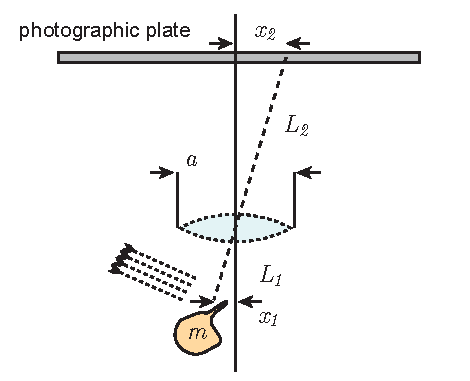
\includegraphics[width = 3.13in]{qmeas_chapter/heismicro}
\end{center}
\caption[Heisenberg microscope]{Heisenberg microscope apparatus.}
\label{fig:heismicro}
\end{figure*}

The Heisenberg microscope is a thought experiment originally described by Werner Heisenberg in 1930 \cite{heisenberg1930physical}.  Although the apparatus described is not at all practical, it does capture all of the critical elements needed to understand the role of the uncertainty principle in the determination of quantum quantities.  Suppose we were interested in attempting to measure the position $x_1$ of a macroscopic object of mass $m$.  We could imagine doing so by scattering some light off of this object and observing the position of the object using a microscope.  The apparatus to do so is shown in Figure \ref{fig:heismicro}.  We imagine attaching a thin rod to the object, whose diameter is less than an optical wavelength.  Presuming we know the approximate position of the object, we can arrange a lens and photographic plate near the object, with the rod close to the focal plane of the lens.  This lens-plate system provides an optical amplification factor of approximately $L_2/L_1$ where $L_1$ is the focal length.

We send in a stream of photons to impinge on the rod, and wait for a single photon to be scattered by the rod, pass through the lens' aperture $a$, and strike the photographic plate, producing a small grain of silver.  The position of this grain $x_2$ can be determined to an accuracy much better than an optical wavelength.  From $x_2$ we can infer the position of the object $x_1 = -x_2 L_1 / L_2$.  However, we cannot make this determination precisely due to the wave nature of light.  The position at which the photon scattered off the rod is not well determined below the spot size of the lens, resulting in an uncertainly in the position
\begin{equation}
\Delta x_{\textrm{measure}} \simeq \frac{1}{2 \pi}\lambda \frac{L_1}{a}.
\label{eq:dxmeas}
\end{equation}
Additionally, because the photon possesses momentum $P = \hbar \omega / c$ and passed through the lens' aperture $a$, it must have transferred to the rod (and thus the attached mass) a random momentum in the $x$ direction with unknown sign and a magnitude on the order of
\begin{equation}
\Delta P_{\textrm{perturb}} \gtrsim \frac{\hbar \omega}{c} \frac{a}{2 L_1} 
\label{eq:dPpert}
\end{equation}
for $a/L_1 \ll 1$.  If we take the product of these two uncertainties, we recover the familiar-looking result
\begin{equation}
\Delta x_{\textrm{measure}} \Delta P_{\textrm{perturb}} \gtrsim \frac{\hbar}{2}.
\label{eq:dxdP}
\end{equation}

This example captures the essential features of any quantum measurement.  We extract information about some observable quantity to within some definite error.  In the process of doing so, we inevitably perturb at least one other quantity of the system---the measurement has some finite \textit{back-action}.  Finally, at some stage of the measurement something \textit{irreversible} occurs (in this case, the measurement photon ceases to exist and a grain of silver is created); this irreversible event is related to crossing the fuzzy boundary between the quantum system under measurement and the classical world we conduct our experiments from.  It is important to note that this \textit{measurement-disturbance} relation is of a fundamentally different nature than the standard position-momentum Heisenberg uncertainty relation, which is the result of the simultaneous measurement of two or more non-commuting quantities.  Here, we only measure one quantity, but the determination of that quantity implies some minimum disturbance to the system under measurement.

One way of understanding the existence of an uncertainty principle for measurement is as an implication of the uncertainty principle applied to the measurement system itself.  Unfortunately, we cannot simply compel a quantum system to reveal its state to us, no matter how loudly we demand it.  By necessity, to measure a quantum system, we must couple that system to some auxiliary system which comprises part or all of a measurement apparatus.  That measurement system itself must also obey the laws of quantum mechanics, which imply that the state of the measurement system must have some finite uncertainty in the preparation of its state.  This uncertainty in the measurement apparatus results in the finite precision of the measurement $\Delta x_{\textrm{measure}}$, and the uncertainty principle then insists that as we reduce the position uncertainty of the object under measurement, the uncertainty in the momentum of the object must increase.

\subsection{The ponderomotive probe for energy}
\label{sec:ponder}

In the case of the Heisenberg microscope, the back-action of the measurement fundamentally influences the future evolution of the quantity we want to determine as the random momentum kick delivered by the photon mixes into the position coordinate through the continued Hamiltonian evolution of the motion of the free mass.  Because of this relationship, if we repeatedly measure the position of the mass by scattering many photons and measuring their displacement, we will not be able to reduce the uncertainty in the position of the free mass to arbitrary precision.  This can be understood as the result of the fact that the eigenstates of the measurement process and the eigenstates of the dynamical evolution of the free mass are not the same.  A state of definite position roughly corresponds to an eigenstate of the measurement.  However, the dynamical evolution of the free mass implies the spreading of a wave packet of definite position.

There is an important class of quantum measurements, called \textit{quantum nondemolition}\footnote{The term quantum nondemolition is perhaps a bit unfortunate and is tangled up with historical ideas of quantum measurements using photons.  Many classes of traditional measurements of quantum systems---for example, detecting photons by absorbing them in a dissipative process such as a photomultiplier tube---literally destroy the system under measurement.  Though physically preserving the system undergoing measurement is a necessary condition for a measurement to be QND, it is hardly sufficient.}
(QND) measurements, that avoid this issue.  If the observed quantity under measurement is itself an eigenstate of the dynamical evolution of the measured system, then reductions in the uncertainty in this quantity will not result in the dynamics of the system mixing the measurement back-action into the measured quantity.
\begin{figure*}
\begin{center}
	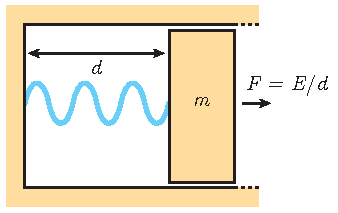
\includegraphics[width = 2.25in]{qmeas_chapter/ponder}
\end{center}
\caption[Ponderomotive probe for energy]{Apparatus for detecting the energy in a cavity resonator by measuring the ponderomotive force on a movable wall.}
\label{fig:ponder}
\end{figure*}
A useful thought experiment that demonstrates all of the important features of a QND measurement is the measurement of the energy in an electrical cavity resonator by measuring the ponderomotive force (i.e. electromagnetic/radiation pressure) that energy exerts on a movable wall of the cavity.  This thought experiment is discussed in Chapter 4 of reference \cite{Braginsky1992}.  A schematic of the setup for this experiment is shown in Figure \ref{fig:ponder}.  We assume that the mass $m$ of the movable wall is large enough that the motion of the wall will be slow compared to the oscillation frequency of the field inside the cavity; in other words, we assume the motion of the wall to be adiabatic.

The ponderomotive force acting on the movable wall of the resonator is $F = E/d$ where $E$ is the resonator's energy and $d$ is a length that is proportional to the size of the resonator and also depends on which resonant mode is excited.  The force $F$ during a measurement of finite time $\tau$ changes the momentum of the wall by $\delta P = E \tau / d$; thus, a measurement of the change in momentum of the wall amounts to a measurement of the energy.  The uncertainty in our determination of the energy of the resonator is proportional to the uncertainty in the initial momentum of the wall, such that
\begin{equation}
\Delta E_{\textrm{measure}} = \frac{d}{\tau} \Delta P.
\label{eq:dEmeas}
\end{equation}
However, the smaller we make the initial uncertainty in momentum, the larger the corresponding uncertainty in the position of the wall $\Delta x$ must be.  An uncertainty in the position of the wall implies an uncertainty in the size $d$ and thus of the resonant frequency of the resonator $\Delta \omega = \omega \Delta x / d$ which in turn produces a random change in the resonator's phase during the measurement
\begin{equation}
\Delta \phi_{\textrm{perturb}} = \Delta \omega \tau = \omega \tau \frac{\Delta x}{d}.
\label{eq:dPhi}
\end{equation}
Combining (\ref{eq:dEmeas}), (\ref{eq:dPhi}), and the uncertainty principle $\Delta x \Delta P \geq \hbar/2$, we obtain the measurement uncertainty relation
\begin{equation}
\Delta E_{\textrm{measure}} \Delta \phi_{\textrm{perturb}} \geq \frac{\hbar \omega}{2}.
\label{eq:dEmeasdPhi}
\end{equation}
We have once again derived an uncertainty relation for the minimum product of our knowledge of the state of the system and the magnitude of the back-action on that system: the more precisely we measure the energy in the resonator, the more uncertain the phase of the oscillation must become.

Unlike in the case of the free particle in the Heisenberg microscope, the observable measured in this experiment (energy) is also a constant of motion of the Hamiltonian of the system under measurement.  The Hamiltonian for the resonator is
\begin{equation}
H = \hbar \omega N
\label{eq:Hres}
\end{equation}
where $N$ is the number of quanta in the resonator.  Eigenstates of the Hamiltonian are of course eigenstates of definite energy, and since the motion of the wall is assumed to be adiabatic, the number of quanta in the resonator does not change.  Thus, by measuring the momentum of the wall for longer and longer times $\tau$ we can reduce the uncertainty in the energy to arbitrary precision.

This measurement possesses all of the properties constituting an ideal quantum measurement.  There is no fundamental constraint on the precision with which we can determine the measured quantity.  Furthermore, the measurement need not itself perturb the quantity under measurement.  The measurement must, however, perturb the quantity which is canonically conjugate to the measured observable in accordance with the uncertainty principle.

\section{Classes of quantum measurements}

In this section I will elaborate some useful distinctions between different classes of quantum measurements.  Specifying which classes of measurements are most relevant to the quantum measurement protocols used in the experiments described in this thesis will serve to focus the remainder of the discussion in the chapter to the theoretical techniques most useful for this subset.

\subsection{Direct and indirect measurements}

Roughly speaking, we can divide any quantum measurement into one of two categories: \textit{direct} and \textit{indirect} measurements.  The difference between the two amounts to where the fuzzy boundary between the classical and quantum worlds is crossed.  In any measurement performed by a laboratory experimenter, some part of the measurement apparatus must obey the laws of classical physics.\footnote{At least, as far as we are presently aware.} The distinction between a direct and indirect measurement is essentially related to how well the quantum system of interest remains safely isolated in the quantum domain.

In a direct measurement, the quantum system undergoing measurement is directly coupled to one or more classical degrees of freedom in the measurement apparatus.  An example of such a measurement is the detection of a photon using a photomultiplier tube.  The arrival of a photon immediately triggers a highly classical cascade of current in the tube, and the quantum system directly sustains any classical back-action from the measurement apparatus (in this case, being completely destroyed).  Since the measurement apparatus is classical and likely contains a large number of degrees of freedom, the back-action of a direct measurement is typically much larger than any minimum bounds set by quantum mechanics.

In contrast to direct measurements, indirect measurements place some auxiliary quantum probe system between the quantum system of interest and the classical measurement apparatus.  The probe system and the main system are brought into contact with one another, allowed to interact for some time, and then decoupled.  The probe system is then brought into contact with the rest of the measurement apparatus, and a direct measurement of the probe is made.  In this way, the excess back-action of the classical measurement is absorbed by the probe system, effectively isolating the main system.  This technique directly permits repeated, minimally-invasive measurements of the main system, using the following procedure.  We first create an ensemble of identically-prepared probe systems.  Each probe system is brought into contact with the main system in series and is then directly measured.  We discard the probe systems after the direct measurement, also discarding the extra back-action of the rest of the measurement apparatus.

There are certain measurements in mesoscopic systems that do not neatly fit into these two categories of direct and indirect measurement.  These are cases where the probe system cannot be described as being firmly classical or firmly quantum.  Even though a measurement may be sensibly described as a direct measurement, the back-action of that measurement may in fact be relatively minimal and non-invasive.  The measurement of a superconducting qubit using a Josephson bifurcation amplifier (JBA) \cite{Vijay2009} is an example of a direct measurement that may not neatly be described as indirect.  The operating principle of the JBA is based on the physics of a nonlinear oscillator; when driven with a very strong drive near the resonant frequency, the dynamics of the oscillator bifurcate into two stable states of very different oscillation amplitude which are quite classically distinguishable.  Moreover, it is not known if the process of switching between these states is reversible or not.  Several experiments \cite{Lupascu2007,Boulant2007} have been performed on this measurement process and have determined that the back-action may be relatively gentle for a measurement which could be considered a direct measurement.

For the remainder of this chapter I will focus exclusively on measurements that fall into the category of indirect measurements.

\subsection{Quantum nondemolition measurements}

Virtually all of the measurements described in the main results of this thesis are quantum nondemolition measurements.  As such, it is important to briefly describe a precise and pleasingly concise definition of the requirements on a measurement process for the measurement to be QND.  The ponderomotive energy probe described in section \ref{sec:ponder} introduced a rough qualitative definition of a QND measurement, namely, that the state of the system corresponding to increasing measurement precision must also correspond to a dynamically stable state of the system's Hamiltonian.  In this section I introduce the most generally used criterion for a measurement to be QND, following the discussion in Chapter 4 of reference \cite{Braginsky1992}.

If we measure some generic observable quantity $q$ of a quantum system, and express the action of the measurement as an operator $U$ which acts on the joint state of the system under measurement and the probe system, we require that the measurement not perturb the quantity undergoing measurement; that is, we require the evolution operator to commute with the measured quantity:
\begin{equation}
[q,U] = 0.
\label{eq:QNDfullsys}
\end{equation}
In other words, the operator $U$ corresponds to the operator for the system we would compute by solving for the full Hamiltonian evolution in time of the coupled system over the entire measurement interval.  This task is in general quite non-trivial, so a slightly less general and more stringent condition for defining a QND measurement is normally used.  Namely, that the Hamiltonian describing the joint evolution of the system and the probe commutes with the measured observable,
\begin{equation}
[q,H_{\textrm{tot}}] = 0.
\label{eq:QNDHtot}
\end{equation}
This condition is more stringent than (\ref{eq:QNDfullsys}), as it implies that $q$ does not change at any point during the measurement, while (\ref{eq:QNDfullsys}) implies that $q$ can evolve during the measurement period but that by the end of the measurement it has returned to its original value.

We can further simplify this criteria by expressing $H_{\textrm{tot}}$ in the very general form
\begin{equation}
H_{\textrm{tot}} = H_{\textrm{obj}} + H_{\textrm{probe}} + H_{\textrm{int}}
\label{eq:Htot}
\end{equation}
where $H_{\textrm{obj}}$ and $H_{\textrm{probe}}$ are free evolution Hamiltonians of the measured system and the probe, respectively, and $H_{\textrm{int}}$ is their interaction Hamiltonian.  Since $q$ is an observable of the measured system and not the probe,
\begin{equation}
[q,H_{\textrm{probe}}] = 0.
\label{eq:qHprobe_com}
\end{equation}
If we assume that $q$ is a constant of motion of $H_{\textrm{obj}}$, then
\begin{equation}
i \hbar \frac{\partial q}{\partial t} +  [q,H_{\textrm{obj}}] = 0.
\label{eq:q_const_motion}
\end{equation}
If $q$ has no explicit time dependence, $\frac{\partial q}{\partial t} = 0$, and by combining (\ref{eq:QNDHtot}), (\ref{eq:qHprobe_com}), and (\ref{eq:q_const_motion}), we arrive at the most common and illuminating definition for a measurement to be QND:
\begin{equation}
[q,H_{\textrm{int}}] = 0.
\label{eq:QND_cond}
\end{equation}
For the remainder of this chapter, I will focus the discussion on measurement theory relevant to QND measurements.

\subsection{Discrete and continuous quantum measurements}

In any physical realization of a quantum measurement, the measurement process will occur over some finite time scale.  This time scale could be the duration of the interaction between the probe system and the main system in an indirect measurement, for example, which results in a single measurement outcome.  We could also imagine a case where we perform many indirect measurements in rapid succession and the cumulative duration of all of these measurements constitute the measurement time scale, compounding the results of all the measurements into a single outcome.  In this latter case, we could also imagine considering the stream of serial measurements as producing a time series of measurement outcomes.  As we continuously integrate these individual measurements, our knowledge of the quantity being measured improves.  Alternatively, we could consider this time series of measurement outcomes as describing a record of the evolution of the measured observable during the measurement period, presuming we have some information about the value of that observable at the beginning of the measurement.

The primary distinction between a discrete measurement and a continuous measurement is essentially a matter of interpretation.  A discrete measurement, resulting in a single estimate of the quantity under measurement, can also be constructed as the integration of a continuous measurement over some finite time to produce a single value.  A continuous measurement can also then be constructed as the continuous limit of a series of rapid discrete measurements performed on a time scale much faster than the evolution time of the quantity being measured.  The measurements comprising the experimental results of this thesis fall into both of these categories.

\section{Ideal and imperfect projective measurements}

The standard textbook description of a quantum measurement involves the instantaneous transition of the quantum state of the measured system from an arbitrary superposition state into a single eigenstate of the measured operator.  The action of the measurement is thus to ``magically'' coerce the system into the joint eigenbasis of the measurement operator and the system.  Repeated textbook measurements yield the same eigenvalue for all measurements after the first measurement.  This process is assumed to be perfect, and always yields a single eigenvalue with certainty, though which eigenvalue is non-deterministic and probabilistically depends on the square of the corresponding eigenvector component of the state vector.

\begin{figure*}
\begin{center}
	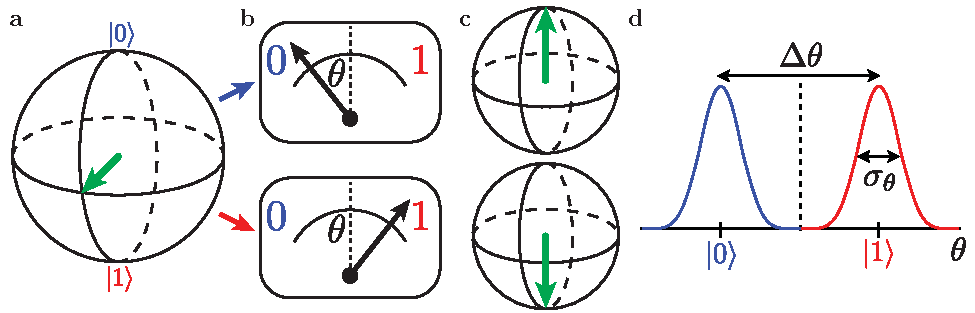
\includegraphics[width = 6.5in]{qmeas_chapter/ideal_proj_meas}
\end{center}
\caption[Ideal projective measurement]{Thought-experimental protocol for an ideal projective measurement. \textbf{a} Bloch sphere representation of a qubit initially prepared in the equal superposition state $(|0\rangle + |1\rangle)/\sqrt{2}$. \textbf{b} An ideal projective measurement is made of the state of the qubit, swinging a classical meter to either the state 0 or 1. \textbf{c} The state of the qubit after the measurement is made is the eigenstate corresponding to the measurement outcome.  \textbf{d} Histogram of many iterations of the thought experiment, showing probability distributions for the angular coordinate of the classical meter.  The finite width of each histogram $\sigma_\theta$ is the result of unavoidable quantum or classical fluctuations of the measurement apparatus.  So long as the separation $\Delta \theta$ is much greater than the histogram width, we can unambiguously map the qubit state to the angular coordinate of the meter, and the measurement is still ideal.}
\label{fig:ideal_proj_meas}
\end{figure*}

It is useful to formulate a picture of an ideal projective measurement for a more realistic case than the straightforward textbook definition.  To simplify the discussion, I will specifically discuss the case of the ideal projective measurement of a two-state quantum system (a qubit).  For some initial coherent qubit state
\begin{equation}
|\Psi\rangle = \alpha |0\rangle + \beta |1\rangle
\label{eq:qubit_psi}
\end{equation}
where $\alpha$ and $\beta$ are complex amplitudes with the normalization condition $|\alpha|^2 + |\beta|^2 = 1$, an ideal projective measurement of the qubit returns the eigenvalue 0 with probability $|\alpha|^2$, and the eigenvalue 1 with probability $|\beta|^2$.  Furthermore, the qubit state following the measurement should be the eigenvector corresponding to the measured eigenvalue.

Without introducing any technical details about the exact nature and form of the overall measurement apparatus, we can construct a fairly general picture of what it means in practice to realize an ideal measurement.  An outline of this measurement is shown in Figure \ref{fig:ideal_proj_meas}.  I will assume that the measurement apparatus is sufficiently precise and optimal to realize a perfect QND measurement with no excess back-action.  The output of the measurement is the angular deflection of a classical, continuous, one-dimensional meter, with two states labelled 0 and 1.

If we repeatedly prepare some initial qubit state---for example, the equal superposition state $|\Psi\rangle = (|0\rangle + |1\rangle)/\sqrt{2}$---and then histogram the results of each measurement, we will recover a set of histograms that look something like the plot shown in Figure \ref{fig:ideal_proj_meas}d.  The histograms corresponding to each state will in general have some finite width due to intrinsic fluctuations (be they classical or quantum) in the measurement apparatus; so long as these fluctuations are significantly smaller than the separation between the histograms, we can unambiguously map the qubit states $|0\rangle$ and $|1\rangle$ onto the meter states 0 and 1.

\begin{figure*}
\begin{center}
	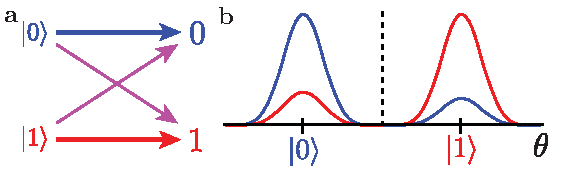
\includegraphics[width = 3.75in]{qmeas_chapter/proj_state_map}
\end{center}
\caption[Projective measurement error due to state mapping]{\textbf{a} Diagram showing the possible permutations of mappings between qubit and meter states, including the error terms in purple. \textbf{b} Ideal measurement histograms, showing the effect of the state mapping errors on measured histograms for the qubit states.}
\label{fig:proj_state_map}
\end{figure*}


Real quantum measurements can deviate from this ideal behavior in a variety of different ways, essentially corresponding to the ways in which the transitions between the panels of Figure \ref{fig:ideal_proj_meas} can go wrong.  First, the mapping between the qubit and meter states could involve non-idealities, schematically shown in Figure \ref{fig:proj_state_map}.  This type of error could be due to some fundamental limitation in the measurement technique which does not produce the ideal state map, thus leaving the qubit and meter in an inconsistent configuration (this fundamentally makes the measurement not perfectly QND).  This type of error could also be the result of imperfections which are not fundamental to the measurement process itself, such as undesired state transitions in the qubit during the measurement, which may or may not leave the qubit and meter in an inconsistent state.

\begin{figure*}
\begin{center}
	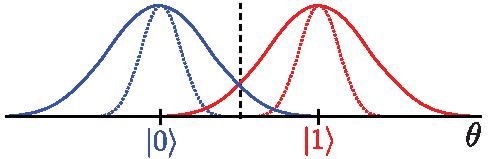
\includegraphics[width = 3.25in]{qmeas_chapter/proj_meas_noise}
\end{center}
\caption[Projective measurement error due to noise]{If the measurement apparatus is noisy, the measurement histograms may be broadened.  If this broadening is large enough to make the histograms overlap, a clear distinction between meter states is no longer possible, introducing a measurement error in the overlap region and possibly making the meter state inconsistent with the qubit state.}
\label{fig:proj_meas_noise}
\end{figure*}

Second, the measurement apparatus itself may be of poor quality and not satisfy the requirement that $\Delta \theta \gg \sigma_\theta$, resulting in measurement histograms that partially overlap, as shown in Figure \ref{fig:proj_meas_noise}.  This type of error is assumed to be entirely related to the function of the measurement apparatus, such that the extra measurement uncertainty is uncorrelated with any quantum measurement uncertainty in the state measurement itself.

Overall, the extent to which a projective qubit measurement accurately captures the quantum state is called the \textit{measurement fidelity}, and is defined based on the action of the measurement on a qubit prepared in one or the other eigenstate.  The fidelity is defined as
\begin{equation}
F = 1 - P(1|0) - P(0|1)
\label{eq:ro_fid}
\end{equation}
where $P(i|j)$ is the probability that the measurement apparatus returned the state $i$ when the qubit was prepared in the state $j$.  A perfect measurement with no errors corresponds to a fidelity of unity.  The worst possible assignment of states in a measurement would be fully random, where $P(0|1) = P(1|0) = 0.5$ and thus $F = 0$.

\section{Ideal and imperfect partial measurements}

Consider for a moment the ideal projective measurement process depicted in Figure \ref{fig:ideal_proj_meas}.  Suppose we have mastered the theory of quantum measurement and we have designed a qubit measurement apparatus that we are very convinced is ideal.  We know for a fact that it performs a QND measurement, applies no excess back-action to the qubit, and the noise in the measurement apparatus is completely limited by minimum bounds set by quantum mechanics.

\begin{figure*}
\begin{center}
	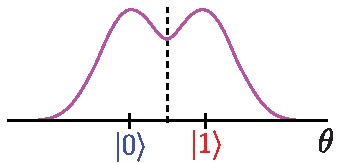
\includegraphics[width = 2.25in]{qmeas_chapter/ideal_partial_meas}
\end{center}
\caption[Partial measurement histograms]{Histogram of the output of the classical meter for an ideal measurement of an ensemble of identically prepared qubit equal superposition states.  The histogram overlap in this case is only due to fundamental quantum fluctuations of the measurement system, not added classical noise.}
\label{fig:ideal_partial_meas}
\end{figure*}

We prepare the qubit in the equal superposition state $|\Psi\rangle = (|0\rangle + |1\rangle)/\sqrt{2}$ and then make a single measurement.  We repeat this state preparation many times, histogramming the results of all of the measurements, resulting in the histogram shown in Figure \ref{fig:ideal_partial_meas}.  Because we have assumed that the measurement apparatus adds no classical noise, this case does not correspond to the noise-broadened projective readout distributions shown in Figure \ref{fig:proj_meas_noise}.  How are we to interpret this distribution?  Moreover, how are we to interpret the outcome of any of the single measurements that make up this distribution?  The answers to these questions lie beyond the textbook definition of quantum measurement.

The measurement just described constitutes a \textit{partial quantum measurement} (sometimes called a \textit{weak quantum measurement}).  Since the histograms for the $|0\rangle$ and $|1\rangle$ states at least partially overlap, we cannot precisely determine which eigenstate the qubit has been projected into.  However, since the overlap is exclusively due to the quantum fluctuations of the measurement apparatus, this uncertainty in the state determination is not merely the result of our crude, classical ineptness---no observer in the universe is able to completely determine that the qubit has been projected into one or the other eigenstate, and, thus, it hasn't been completely projected at all!

The state of the qubit has, in fact, evolved as a result of the measurement, in some manner consistent with the measurement outcome (just as in a projective measurement).  However, unlike in a perfect projective measurement, we are now faced with a continuum of possible measurement outcomes, where each possible value is correlated with a particular measurement back-action on the qubit state.  For a projective measurement, this back-action is the usual act of projecting the qubit into the eigenstate consistent with the meter outcome.  To determine the equivalent mapping between this new continuous spectrum of meter outcomes and the resulting back-action, we will need to first develop some statistical tools.

It could of course be possible that all of the histogram overlap is not due to the intrinsic quantum fluctuations of the measurement apparatus.  If some of the overlap is due to additional classical noise in the measurement, as in Figure \ref{fig:proj_meas_noise}, we cannot disentangle the added fluctuations from the intrinsic fluctuations and our measurement is no longer perfect.  In this case, we will not be able to create an ideal mapping between measurement outcomes and back-action on the qubit, but rather some of this back-action must be expressed as a decrease in the purity of the ensemble qubit state as a result of the measurement.  The quality of a measurement apparatus in this case is described by a \textit{quantum efficiency} $\eta$, where $\eta$ is qualitatively given as the ratio of the size of the quantum fluctuations to the size of the total fluctuations in the measurement apparatus.  This concept will be made more concrete shortly.



\subsection{Quantum Bayesian inference}\label{s:bayesian}

Partial quantum measurements, where we acquire some finite and incomplete information about the state of a quantum system from a measurement, are a natural fit for analysis using Bayesian statistics.  We start with some initial estimate of the density matrix describing the system under measurement; if we have no initial information, this density matrix will be essentially a maximum-entropy placeholder.  We perform a partial measurement, and then use the result of that measurement to update our best estimate of the new density matrix conditioned on the measurement outcome.  If we have realized a perfect quantum measurement apparatus, then the measurement outcome should perfectly correlate with the coherent evolution of the density matrix as a result of the measurement, enabling the perfect tracking of a known initial state.

The quantum Bayesian (QB) approach \cite{qu_bayes,koro11} is relatively modern compared to other more traditional theoretical frameworks for understanding partial measurements such as positive operator-valued measures (POVM) .  The QB approach has the advantage of being relatively straightforward to calculate compared to POVMs, and I personally find it to provide more illuminating insight into how our state of knowledge evolves as the result of a partial measurement.  All of the experimental results described in this thesis are well modeled in the QB framework, and as such I will not explicitly discuss POVMs but rather refer to a excellent treatment on the subject for further reading \cite{jaco06}.

If we presume that we begin the experiment described in Figure \ref{fig:ideal_partial_meas} with an ensemble of qubits identically prepared in the state $|\Psi\rangle = (|0\rangle + |1\rangle)/\sqrt{2}$, we can describe the state of that ensemble with the density matrix
\begin{equation}
\rho(t=0) = \frac{1}{2} \left( \begin{array}{cc}
1 & 1 \\
1 & 1 \end{array} \right)
\label{eq:rho_equal}
\end{equation}
in the $\sigma_z$ basis.  The diagonal entries in this matrix represent the classical probability for finding the system in one or the other eigenstate, while the off-diagonal elements indicate the extent to which the ensemble exists in a superposition of eigenstates.  Because the diagonal elements can be naturally interpreted as classical probabilities, we can apply Bayes' rule to update these values following a partial measurement, calculating the probability to find the qubit in one or the other eigenstate conditioned on the Bayesian estimate of that probability.  Bayes' rule captures the essential procedure for updating our state of knowledge of a system based on some new (incomplete) piece of information acquired about that system:
\begin{equation}
P(A|\beta) = \frac{P(\beta|A) P(A)}{P(\beta)}
\label{eq:bayes_rule}
\end{equation}
where the conditional probability to find the system in the state $A$ given some new measurement result $\beta$ is equal to the probability of having gotten the outcome $\beta$ if the state is in fact $A$ multiplied by our current best estimate for the probability of the system being in the state $A$.  The denominator is a normalization factor.

In the measurements described in this thesis, the coordinate that represents the output of our classical meter will be a voltage $V$ rather than an angle $\theta$, so I will use $V$ for consistency.  Applying \ref{eq:bayes_rule} to the situation at hand results in the following update to the density matrix diagonal elements following a measurement which produces the outcome $V$:
\begin{equation}
P(i|V) = \rho_{ii}(t) = \frac{P(V|i)P(i)}{P(V)}
\label{eq:Pi_update}
\end{equation}
where $P(i)$ is the probability to measure the state $|i\rangle$, given by $\rho_{ii}(t=0)$, and $P(V)$ is the probability to have observed the measured outcome $V$, given by a weighted prior probability distribution conditioned on our knowledge of the initial state $\rho$ and the distribution of measurement outcomes for the states 0 and 1 ($P(V)$ is the distribution plotted in Figure \ref{fig:ideal_partial_meas}).  If we assume that the probabilities of measuring a particular value $V$ when the qubit is prepared in the ground or excited state are normalized Gaussian distributions of width $\sigma$ centered around $\pm \Delta V/2$,  then
\begin{align}
\rho_{11}(t) &= \frac{\rho_{11}(0)}{P(V)}  \exp {\left( \frac{-(V - \Delta V/2)^2}{2\sigma^2} \right)} \label{eq:Pi_update_gauss_11} \\
\rho_{00}(t) &= \frac{\rho_{00}(0)}{P(V)}  \exp \left( \frac{-(V + \Delta V/2)^2}{2\sigma^2} \right)
\label{eq:Pi_update_gauss_00}
\end{align}
where $P(V)$ is given by our prior knowledge of the qubit state
\begin{equation}
P(V) = \rho_{00}(0)  \exp{\left( \frac{-(V + \Delta V/2)^2}{2\sigma^2} \right)} + \rho_{11}(0) \exp{\left( \frac{-(V - \Delta V/2)^2}{2\sigma^2} \right)}
\end{equation}
and the width $\sigma$ is assumed to be the result of averaging a white noise background with power spectral density $S$ for the measurement time $t$ such that $\sigma^2 = S/2t$ \cite{koro11}.

We can now interpret the experimental distribution from Figure \ref{fig:ideal_partial_meas}.  With $\rho_{00}(0) = \rho_{11}(0) = 1/2$, $P(V)$ is the equally weighted sum of the two Gaussian distributions.  If the measurement value $V$ is exactly equal to 0, $P(V)$ is equal to the exponential term in \eqref{eq:Pi_update_gauss_11} and $\rho_{11}(t) = \rho_{11}(0)$.  Remarkably, in this case, we have made a partial measurement of the state of the qubit which has provided us with \textit{exactly zero information} about which state it is in!  Because we have learned nothing new about the state, there should be no corresponding back-action due to this measurement, reflected in the fact that the density matrix elements have not changed.

If $V>0$, the exponential term in \eqref{eq:Pi_update_gauss_11} will be larger than the exponential term in \eqref{eq:Pi_update_gauss_00}, so $\rho_{11}(t) > \rho_{11}(0)$.  In other words, because this value of $V$ corresponds to an outcome which is more likely if the qubit is in the excited state, the back-action of the measurement must have kicked the state towards $\ket{1}$.  Also note that if $\rho_{ii}(0) = 1$, $\rho_{ii}(t) = 1$ regardless of the measurement outcome.  This is exactly what we expect for a QND measurement: if the qubit is in an eigenstate, the back-action of the measurement should not disturb this eigenstate.  Furthermore, a repeated measurement of an initial superposition state will eventually drive the qubit into one or the other eigenstate, realizing a projective measurement.

If the only back-action of the measurement process is the evolution of the qubit towards one of its eigenstates (leaving the phase of the qubit state unchanged), and we have realized an ideal measurement, then the resulting change in the off-diagonal elements of the density matrix must be completely specified by the change in the diagonal elements:
\begin{equation}
\rho_{01}(0) = e^{i\phi} \sqrt{\rho_{00}(0) \rho_{11}(0)} \quad \rho_{01}(t) = e^{i \phi} \sqrt{\rho_{00}(t) \rho_{11}(t)} 
\end{equation}
implying
\begin{equation}
\rho_{01}(t) = \rho_{01}(0) \frac{ \sqrt{ \rho_{00}(t) \rho_{11}(t)} } { \sqrt{ \rho_{00}(0) \rho_{11}(0)} }.
\label{eq:rho01_update}
\end{equation}
This Bayesian state update procedure and the resulting ability to track a qubit state undergoing measurement has been extensively tested experimentally at QNL \cite{Weber2014,murch_observing_2013,Weber2014a}, demonstrating excellent agreement with theoretical predictions.

It might seem unintuitive at first that we can write down such a simple and seemingly deterministic set of equations for the evolution of the qubit state as the result of a measurement.  The measurement result $V$ is of course still stochastic and unpredictable; however, because we have presumed a perfect, quantum-limited measurement apparatus, and we begin with a known density matrix, the purity of the qubit state need not change as a result of the measurement as no information about the qubit state has been lost or discarded.  Thus, the back-action on the qubit state is perfectly correlated with the measurement result, and the only effect of quantum uncertainty is the unpredictable nature of which measurement result we find.

The ensemble dephasing rate associated with this measurement process, obtained by averaging \eqref{eq:rho01_update} \cite{koro11}, is
\begin{equation}
\Gamma = \frac{(\Delta V)^2}{4S}.
\label{eq:bayesian_dephasing}
\end{equation}
The term ``dephasing'' here is something of a misnomer, as we just asserted that the action of this measurement does not change the phase of a superposition state.  In the ensemble picture, the stochastic evolution of a superposition state towards one of the eigenstates is indistinguishable from stochastic evolution of a superposition state around the equator of the Bloch sphere, so this process is still called dephasing.  At the level of a particular measurement, however, the two processes are fundamentally different, as we will see in a specific example in section \ref{s:cQED_backaction}.  This rate can also be naturally interpreted as the ``strength'' of a measurement; a stronger measurement projects a superposition state into an eigenstate more rapidly, and thus the apparent ensemble dephasing rate is larger.

Remarkably, this fairly straightforward picture actually corresponds very closely to the quantum measurements realized in this thesis.  The primary departure from this idealized picture is that the measurements are not entirely perfect, but rather involve some finite information collection efficiency $\eta < 1$.  This loss of information looks exactly like an extra dephasing of the qubit state characterized by a rate $\gamma$ which depends on $\eta$ and other factors specific to a particular measurement apparatus; to include this effect we simply multiply (\ref{eq:rho01_update}) by an exponentially decaying term $e^{-\gamma t}$ and add $\gamma$ to the right side of \eqref{eq:bayesian_dephasing}.  We can write a simple functional form for the efficiency as
\begin{equation}
\eta = \Gamma_m / \Gamma_{\rm tot}
\label{eq:eta_basic_form}
\end{equation}
where $\Gamma_m$ is the ideal dephasing rate associated with a perfect quantum measurement, while $\Gamma_{\rm tot}$ is the total dephasing measured in a given experiment.  A perfect quantum measurement thus corresponds to $\Gamma_{\rm tot} = \Gamma_m$; additional dephasing from other sources (be it imperfect information collection or dephasing intrinsic to the non-ideal quantum system itself) increases $\Gamma_{\rm tot}$ and thus reduces $\eta$.

\section{Continuous quantum feedback control}

With the Bayesian framework in place to track the evolution of a quantum state undergoing measurement, we can consider utilizing the record of this evolution to actively steer the state towards some desired value using feedback. The basic idea of feedback control is predicated on the assumption that we can measure the state of a system precisely, compare that state to some desired target state, and use our measurement to condition a control signal to steer the system towards the desired state and stabilize it against disturbances.  In classical feedback control this process is relatively straightforward, as our measurement of the system need not disturb the state of that system.  In quantum feedback control, this assumption is fundamentally violated by the measurement-disturbance relations which have been the subject of much of the rest of this chapter.

\begin{figure*}
\begin{center}
	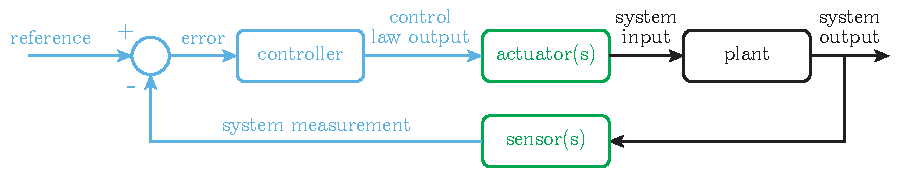
\includegraphics[width = 6in]{qmeas_chapter/feedback_diagram}
\end{center}
\caption[Generic feedback control system]{Block diagram of a generic feedback control system.  The control portion of the system is drawn in blue, the interface between the control and the plant in green, and the plant itself in black.}
\label{fig:feedback_diagram}
\end{figure*}

A generic diagram of a feedback control scheme is shown in Figure \ref{fig:feedback_diagram}.  Consider a system (usually called the \textit{plant}, in a reference to the broad industrial applicability of feedback control) with one or more \textit{sensors} which measure some outputs of the system.  The sensor outputs are subtracted from some \textit{reference} values, producing an error signal that parameterizes the difference between the target state of the system and the current state of the system.  This error is fed into a \textit{controller} which applies some \textit{control law} to the error signal, producing a set of control signals which are fed to one or more \textit{actuators} which apply the control signals to the plant.  Some generic questions control theory asks and answers about this type of system are, for instance, is a particular control law unstable, stable for some parameters, or unconditionally stable?  What control law provides the best control performance, and can a particular control law be shown to be \textit{optimal} in some sense?

In classical control theory, there is no fundamental reason that the precision with which a property of the plant is measured should be of relevance to the dynamical evolution of the plant.  There may be unavoidable noise in the measurements of the plant, but increasing the strength of a measurement should have no result besides increasing the size of the signal relative to this noise.  In quantum measurement, performing a stronger measurement inevitably increases the disturbance on the plant.  Therefore, quantum control theory is faced with additional complexity in analyzing the performance of control laws, especially with regards to optimality.  Measuring a system more strongly may increase the disturbance to such a level that the resulting fluctuations are beyond the ability of the actuators to compensate, for example.  Explicit details on the general methods of quantum control are beyond the scope of relevance for this thesis; see reference \cite{qmcontrol_book} for further reading on the subject.

Besides the additional theoretical complexity of the measurement-disturbance tradeoff, demonstrating quantum feedback control is a significant technological challenge.  We require a system which implements a nearly ideal, variable strength partial quantum measurement, as we will be interested in assessing theoretical items of interest such as the measurement strength which produces optimal control.  If the aim of our feedback control is, for example, the stabilization of an arbitrary qubit state, a projective measurement would immediately destroy the stabilized state.  Experimental systems that meet this demand have only recently been realized, and as such the first two demonstrations of quantum feedback control did not occur until 2011: the stabilization of photon number states in a microwave cavity \cite{haroche_fb}, and the experiment described in this thesis.

\subsection{Stabilization of Rabi oscillations of a qubit}

I will not attempt to lay out some general framework in which to pose the particular quantum control experiment realized in this thesis; I will instead launch into specifics.  The plant will be a qubit described by a density matrix $\rho(t)$, and our control law will aim to stabilize the dynamics of the density matrix in the presence of dephasing.  Specifically, we will continuously drive Rabi oscillations of the qubit and aim to stabilize the phase of these oscillations.  Without yet going into details of the experimental implementation, the sensor output corresponds to a continuous partial measurement of $\langle \sigma_z \rangle$.  The actuator will correspond to the frequency at which we drive Rabi oscillations $\Omega_r$; to correct the phase of the qubit oscillations, we briefly adjust $\Omega_r$ to speed or slow the oscillations.  Our reference signal will be a high-quality classical oscillator oscillating at a target frequency $\Omega_0$, and the error signal will be the phase difference between this reference and the measured phase of the oscillations of $\langle \sigma_z \rangle$.  This setup can be intuitively thought of as a phase-locked loop, though here we are stabilizing the phase of a quantum oscillator.

The theory for this control scheme was formulated by Korotkov in reference \cite{korotkov_dir_fb}.  It is worth nothing that this work was published in 2002 yet it took another 9 years for quantum measurement technology to advance sufficiently to realize it.  My discussion here will more closely follow the discussion in our publication on the experiment \cite{vijay_stabilizing_2012}; specifically, section IV of the supplementary materials.

We will first consider the case where the detector is ideal ($\eta=1$). The qubit evolution during the process of continuous measurement can be described using stochastic equations \cite{Korotkov2001} for the qubit density matrix $\rho$. Stochastic equations are required because the measurement outcome $V(t)$ will fundamentally involve a random variable corresponding to the quantum fluctuations of the measurement apparatus; these expressions are essentially the result of taking the time derivatives of (\ref{eq:Pi_update_gauss_11}) and (\ref{eq:Pi_update_gauss_00}).   The measurement output signal $V(t)$ is given by
\begin{equation}
V(t) = \frac{\Delta V}{2} [\rho_{11}-\rho_{00}] + \xi_{\mathrm{id}}(t)
\label{meas_I}
\end{equation}
where $\xi_{\mathrm{id}}$ is the white noise of an ideal detector characterized by the (one-sided) spectral density $S_{\mathrm{id}}$.  The strength of the measurement, characterized by the measurement induced dephasing rate \eqref{eq:bayesian_dephasing}, is given by
\begin{equation}
\Gamma_{\varphi}=\frac{(\Delta V)^{2}}{4S_{\mathrm{id}}}.
\end{equation}
For a resonant Rabi drive, the stochastic equations describing the evolution of the density matrix under simultaneous driving and measurement (in Stratonovich form) are given by
\begin{equation}
 \dot{\rho}_{11}=-\dot{\rho}_{00}=-\Omega _{\mathrm{R}}\mathrm{Im}\rho_{01}+\rho _{11}\rho _{00}\frac{2\Delta V}{S_{\mathrm{id}}}V(t)-\Gamma_{1} \rho_{11},  \label{Bayes_11}
\end{equation}
\begin{equation}
\dot{\rho}_{01} =i\frac{\Omega _{\mathrm{R}}}{2}\left( \rho _{11}-\rho_{00}\right) -\frac{\Delta V}{S_{\mathrm{id}}}\rho _{01}\left( \rho _{11}-\rho_{00}\right) V(t) -(\Gamma _{\mathrm{env}} + \frac{\Gamma_{1}}{2})\rho _{01},  \label{Bayes_01}
\end{equation}
where $\Gamma _{\mathrm{env}}$ is the environmental dephasing rate and $\Gamma_{1}$ is the qubit energy relaxation rate \cite{korotkov_dir_fb}.

The terms in \eqref{Bayes_11} can be understood as follows.  The first term describes the deterministic state rotation due to the Rabi drive.  The second term describes the stochastic back-action of the measurement on the qubit state.  The prefactor $\rho_{00}\rho_{11}$ is maximal when $\rho_{00} = \rho_{11} = 1/2$, and decreases to zero when either term is zero.  Thus, the measurement has no effect if the qubit is already in an eigenstate, exactly what we expect for a QND measurement.  Otherwise, the measurement stochastically drives the state towards one or the other eigenstate.  The third term models spontaneous energy relaxation from the excited state to the ground state.  The terms in \eqref{Bayes_01} are similar.  Note that the factor $( \rho _{11}-\rho_{00})$ enforces the evolution described by \eqref{eq:rho01_update}.  The third term describes the decoherence of the state due to both intrinsic environmental dephasing $\Gamma_{\rm env}$ and energy relaxation $\Gamma_1$.

To obtain a closed form expression for the action of feedback control, it is possible to reduce the number of qubit degrees of freedom down to only one.  First, because a resonant Rabi drive rotates the qubit about the $x$-axis and our measurement does not alter the phase of a superposition state, the qubit state is restricted to the $x=0$ plane. Second, by neglecting energy relaxation, we can consider the qubit state as pure, ascribing any measurement inefficiency ($\eta<1$) to some additional noise at the detector output \cite{Kor-nonideal}.  We set $\Gamma_{\rm env}=0$ in equation (\ref{Bayes_01}) and model both environmental dephasing and detector inefficiency by adding a noise term $\xi_{\mathrm{add}}(t)$ to equation (\ref{meas_I}), resulting in the measurement outcome
\begin{equation}
V(t) = \frac{\Delta V}{2} [\rho_{11}-\rho_{00}] + \xi_{\mathrm{id}}(t) + \xi_{\mathrm{add}}(t),
\label{meas_I_analytic}
\end{equation}
where $\xi_{\mathrm{add}}(t)$ has a spectral density $S_{\mathrm{add}} = S_{\rm out} - S_{\rm id}$, where $S_{\rm out} = S_{\rm id}/\eta$ is the total output noise. Therefore, the qubit state evolution can be described by only one parameter, the polar (zenith) angle $\theta(t)$ on the Bloch sphere:
\begin{equation}
\xpec{\sigma_z}(t)= \cos [\theta(t)], \,\,\, \xpec{\sigma_y}(t)=\sin[\theta(t)], \,\,\, \xpec{\sigma_x}(t)=0.
\end{equation}

The goal of the feedback is to stabilize the Rabi oscillation to the form $\theta(t)=\Omega_0 t$ with a fixed frequency $\Omega_0$. We characterize the feedback efficiency $D$ \cite{korotkov_dir_fb} as
\begin{equation}
D=\overline{\cos [\theta_{\rm err}(t)]}, \,\,\, \theta_{\rm err}(t) = \theta(t)-\Omega_0 t,
\end{equation}
which corresponds to the time-averaged scalar product of the desired and actual state vectors on the Bloch sphere.  The qubit ``phase shift error'' $\theta_{\rm err}$ evolves as \cite{korotkov_dir_fb}
\begin{equation}
\dot\theta_{\rm err} = -\frac{\Delta V}{S_{\rm id}} \sin \theta \left(\frac{\Delta V}{2}\cos \theta +\xi_{\rm id}\right).
\label{evol}
\end{equation}
In order to compensate this dephasing-induced phase shift, we now apply feedback by modulating the frequency of the Rabi drive with a feedback term $\Omega_{\rm fb}(t)$ as
\begin{equation}
\Omega_{\rm R}(t) =\Omega_0+\Omega_{\rm fb} (t).
\label{fb0}
\end{equation}
The control law is a simple proportional control, which Korotkov refers to as the ``direct feedback'' control law:
\begin{equation}
\frac{\Omega_{\rm fb}(t)}{\Omega_0} = F \frac{4}{\Delta V} \,\sin (\Omega_0 t) V(t - \tau_{\rm delay}).
\label{fb}
\end{equation}
Here $F$ is the dimensionless feedback gain and the choice of the normalization factor $4/\Delta V$ corresponds to $\Omega_{\rm fb}/\Omega_0=-F\sin\theta_{\rm err}$ on average.  The extra term $\tau_{\rm delay}$ in the argument of $V$ accounts for the fact that in general our measurement and feedback control will have some finite bandwidth, so that the control correction we apply to the system at time $t$ actually corresponds to a measurement made at some earlier time, delayed by $\tau_{\rm delay}$.  For the moment we assume this delay to be negligibly small.

The qubit evolution (\ref{evol}) is written in the Stratonovich form; converting it into the It\^o form (for averaging) we obtain the extra term $[(\Delta V)^2/4S_{\rm id}]\sin\theta\cos\theta$, which comes from the measurement part of (\ref{evol}). However, this extra term in the It\^o form is not important because we average the evolution of the phase shift $\theta_{\rm err}$ over the Rabi period. The averaging is simple when $\theta_{\rm err}$ evolves slowly, so that $\theta_{\rm err}$ is uncorrelated with $\theta$. Thus, we need to assume weak coupling, $\Gamma \ll \Omega_0$ and weak feedback, $F\ll 1$. Averaging cancels the product $\sin\theta\cos\theta$ and replaces $\sin(\Omega_0 t)\cos\theta$ with $-(\sin\theta_{\rm err} )/2$; thus we obtain
\begin{align}
\dot\theta_{\rm err} = &\left( \frac{4F\Omega_0}{\Delta V} \sin(\Omega_0 t) -\frac{\Delta V}{S_{\rm id}} \sin (\Omega_0 t+\theta_{\rm err}) \right) \xi_{\rm id} \notag \\
&+ \frac{4F\Omega_0}{\Delta V} \, \sin (\Omega_0 t) \,    \xi_{\rm add}  -F\Omega_0 \sin\theta_{\rm err}.
\label{evol-main}
\end{align}

In this equation, the last term attracts the phase shift $\theta_{\rm err}$ to zero, while the noise terms cause diffusion of $\theta_{\rm err}$. Examining the term in large parentheses, it is clear why there is an optimum value of the feedback gain $F$. For example, for an ideal detector ($\xi_{\rm add}=0$), the effect of the noise $\xi_{\rm id}$ can be compensated when $4F\Omega_0/\Delta V = \Delta V/S_{\rm id}$, leading asymptotically to full synchronization, $\theta_{\rm err}(t)=0$. This compensation has been studied previously \cite{Hofmann_qcontrol,state_stable} in the context of stabilizing the qubit state on a fixed point on the Bloch sphere.

Next, we average the noise in (\ref{evol-main}) over a Rabi period to eliminate the oscillatory components. We can replace $\sin (\Omega_0 t)\,\xi_{\rm add}$ with $\tilde\xi_{\rm add}/\sqrt{2}$, where $\tilde\xi_{\rm add}$ is white noise with the same spectral density as $\xi_{\rm add}$. Averaging the term with $\xi_{\rm id}$ is similar, but slightly more cumbersome. We first rewrite it as $[A\cos (\Omega_0 t)+B\sin(\Omega_0 t)]\xi_{\rm id}$ with $A=-(\Delta V/S_{\rm id})\sin\theta_{\rm err}$ and $B=4F\Omega_0/\Delta V -(\Delta V/S_{\rm id})\cos\theta_{\rm err}$. Averaging over a Rabi period then gives $\sqrt{(A^2+B^2)/2} \, \tilde\xi_{\rm id}$ with a similar white noise, $S_{\tilde{\xi}_{\rm id}}=S_{\rm id}$. We now add the uncorrelated contributions from the noises $\tilde\xi_{\rm id}$ and $\tilde\xi_{\rm add}$, and convert the result into a noise $C\,\tilde\xi_{\rm out}$, where $\tilde\xi_{\rm out}$ has the same spectral density $S_{\rm out}$ as the output noise and $C^2=\eta(A^2+B^2)/2+(1-\eta)(4F\Omega_0/\Delta V)^2/2$. This allows us to replace (\ref{evol-main}) with
\begin{align}
\dot\theta_{\rm err} =  -F\Omega_0 \sin\theta_{\rm err} + C \, \tilde \xi_{\rm out}, \,\,\,\, S_{\tilde \xi_{\rm out}}= S_{\rm out} , \label{evol-eff}\\
C^2= \frac{2F\Omega_0}{S_{\rm out}} \left( \frac{1}{\eta}\, \frac{F}{\Gamma/\Omega_0} +\frac{\Gamma/\Omega_0}{F}-2\cos\theta_{\rm err} \right) .
\label{C-def}
\end{align}

This is a Langevin equation, and the corresponding Fokker-Planck equation for the probability distribution $P(\theta_{\rm err}, t)$ is
\begin{equation}
\frac{\partial P}{\partial t}= \frac{\partial (F\Omega_0\sin\theta_{\rm err} \, P)} {\partial \theta_{\rm err}} + \frac{1}{4}\, \frac{\partial^2 (C^2 S_{\rm out} P)}{\partial \theta_{\rm err}^2},
\label{F-P}
\end{equation}
where $P(\theta_{\rm err})$ is $2\pi$ periodic and is normalized as $\int_{-\pi}^{\pi} P(\theta_{\rm err})\,d\theta_{\rm err} =1$. The stationary solution $P_{\rm st}(\theta_{\rm err})$ then satisfies the equation
\begin{equation}
\frac{d(C^2 S_{\rm out} P_{\rm st})}{d\theta_{\rm err}} + 4F\Omega_0\sin\theta_{\rm err}\, P_{\rm st} ={\rm const}=0,
\end{equation}
where the constant is zero because of the symmetry between $\theta_{\rm err}$ and $-\theta_{\rm err}$. Using the $C^2(\theta_{\rm err})$ dependence from (\ref{C-def}), we get
\begin{equation}
P_{\rm st}(\theta_{\rm err})= p_0 \left( \frac{1}{\eta}\, \frac{F}{\Gamma/\Omega_0} +\frac{\Gamma/\Omega_0}{F}-2\cos\theta_{\rm err} \right) ^{-2},
\label{P_st}
\end{equation}
where $p_0$ is a normalization constant.

Finally, from the stationary probability distribution for
the phase shift $\theta_{\rm err}$, we calculate the feedback efficiency as
$D=\int_{-\pi}^\pi \cos\theta_{\rm err}\, P_{\rm st}(\theta_{\rm err}) \, d\theta_{\rm err}$
and thus obtain the analytical formula
\begin{equation}
D=\frac{2}{\displaystyle \frac{1}{\eta}\, \frac{F}{\Gamma/\Omega_0}+\frac{\Gamma/\Omega_0}{F}}.
\label{D-res}
\end{equation}
From (\ref{D-res}) it is straightforward to calculate the optimal value of the feedback gain $F$ and corresponding maximum value for $D$:
\begin{equation}
F_{\rm opt}=\sqrt{\eta} \, \frac{\Gamma}{\Omega_0} , \,\,\,  D_{\rm max}=\sqrt{\eta}.
\label{optimum}
\end{equation}
Notice that $F_{\rm opt}\ll 1$ for weak coupling ($\Gamma\ll \Omega_0$) so the assumption of weak feedback $F\ll 1$ is satisfied.

The existence of an optimal feedback strength is quite intuitive.  Intrinsically, the goal of the feedback loop is to correct for the (partially) known stochastic back-action of the measurement process.  In the ideal case $\eta = 1$, $F_{\rm opt}$ is just given as the ratio of the total dephasing rate and the Rabi frequency.  From \eqref{fb} we can think of $F$ as parameterizing the strength of the feedback in terms of the fractional shift in $\Omega_0$.  Considering that $\Gamma/\Omega_0$ is essentially the fractional disturbance, it makes sense that the size of the feedback correction should be identical to the size of the disturbance.  In the non-ideal case $\eta < 1$, only the fraction of the feedback amplitude $\sqrt{\eta}$ actually corresponds to the quantum back-action of the measurement, while the remainder is uncorrelated classical noise.  Thus, a reduced feedback strength is necessary to re-scale the total correction to properly correct the fraction of the fluctuations which are correlated with the qubit state.  However, because the uncorrelated part of the signal is still applied to the qubit, the efficiency of the feedback is limited by the same fractional correlation $\sqrt{\eta}$.













\chapter{Superconducting qubits and circuit quantum electrodynamics}
\label{c:scqb}

Having discussed the framework of partial, continuous, idealized quantum measurements, I will now describe the physical system we use to realize such measurements.  Rather than utilize a natural quantum system (such as an atom or single spin), we utilize engineered superconducting circuits which are described by the same quantum mechanics as natural quantum systems.  These circuit platforms have some significant advantages, especially the design flexibility in choosing various coupling strengths (created here through structures such as capacitors rather than natural dipole moments or spin-spin couplings).

\section{Quantization of electrical circuits}

The fact that electrical circuits can behave as coherent quantum variables is somehow simultaneously surprising and obvious.  It is standard practice to find a quantum description of a mechanical system by writing down the classical Lagrangian and Hamiltonian descriptions of the system, introducing commutation relations to the canonically conjugate degrees of freedom, and finally promoting these degrees of freedom to quantum operators.

For mechanical systems of rigid bodies it feels somewhat natural to consider these bodies as ``particles" and write down a quantum Hamiltonian and wavefunction for their motion, as their rigid-ness implies we can imagine all of their microscopic degrees of freedom moving together.  Of course, for large, classical objects, this description would in reality break down due to decoherence at some level. Still, experiments are continuously pushing the quantum description of mechanical rigid bodies to larger and larger objects, consisting of billions of atoms all moving together coherently in one mechanical mode \cite{Rocheleau2010,OConnell2010,Palomaki2013}.  Electrical circuits, on the other hand, consist of a large number of charge carriers, and in general there is no particular reason to believe that the quantum motion of these charge carriers should be strongly correlated to enable a similar description of their collective motion as a rigid body.

\subsection{Superconductivity}

Electrical circuits composed of superconducting materials provide a context in which it makes perfect sense to consider the motion of all of the charge carriers together as analogous to a mechanically rigid body.  Below the transition temperature in a conventional superconductor, the electrons pair to form bosonic composite particles known as Cooper pairs \cite{tinkham2004introduction}.  At very low temperature, all of these bosonic particles cool into a single collective ground state.  The excitation spectrum of the system then has a large energy gap $2 \Delta$ between the ground state and the first excited state, corresponding to the energy needed to dissociate a Cooper pair back into two electrons.

This gapped excitation spectrum is the origin of the most well known phenomenological behavior of superconductors: current flow without resistance.  The microscopic origin of resistance in a normal metal conductor is the scattering of electrons off of defects in the metal into other conduction states, corresponding to energy exchange with the lattice.  Because of the large energy gap in the spectrum of a superconductor, there are no nearby states available for Cooper pairs to scatter into, enabling the ideal flow of current without the charge carriers exchanging energy with defects in the metal.  Thus, it becomes perfectly natural to model the collective behavior of all Cooper pairs occupying the ground state as a single wavefunction.

\subsection{Quantization of an LC oscillator}

For the purposes of this thesis, a derivation of quantum circuit operators in the context of an LC oscillator will suffice.  For a more general discussion of the subject see reference \cite{Devoret1995}.

\begin{figure*}
\begin{center}
	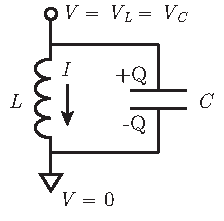
\includegraphics[width = 1.5in]{scqb_chapter/LC_osc}
\end{center}
\caption[LC oscillator circuit diagram]{LC oscillator quantities and coordinates.}
\label{fig:LC_osc}
\end{figure*}


A circuit schematic of an LC oscillator is shown in Figure \ref{fig:LC_osc}.  The classical equations of motion for an LC oscillator are usually derived using the voltage and current as the generalized coordinates.  For a quantum treatment of an LC oscillator and for quantum circuits in general it turns out to be more convenient to use the charge on the capacitor and the flux threading the inductor as the coordinates.  Fundamentally, this is because in some circuits the number of charge-carrying quanta on a metal island turns out to be a good quantum number, and in some others the total number of superconducting flux quanta threading some loop turns out to be a good quantum number.  We can write the total energy in the oscillator in the standard way as
\begin{equation}
E = \frac{1}{2} C V^2 + \frac{1}{2} L I^2.
\label{eq:LC_E}
\end{equation}
Converting to charge and flux using the relations $Q = VC$ and $\Phi = LI$, we can write the classical Hamiltonian of the LC oscillator as
\begin{equation}
H = \frac{\Phi^2}{2L} + \frac{Q^2}{2C}.
\label{eq:LC_H}
\end{equation}
Writing Hamilton's equations of motion
\begin{equation}
\frac{\partial H}{\partial \Phi} = \Phi/L = I = -\dot{Q} \quad \quad \frac{\partial H}{\partial Q} = Q/C = L\dot{I} = -\dot{\Phi}
\label{eq:LC_hams}
\end{equation}
we can immediately identify $\Phi$ as a generalized position and $Q$ as a generalized momentum, promote them to quantum operators $\hat{\Phi}$ and $\hat{Q}$, and write their commutation relation
\begin{equation}
[\hat{\Phi},\hat{Q}] = i \hbar.
\label{eq:LC_comm}
\end{equation}
Thus, the quantum dynamics of an LC oscillator are those of a quantum harmonic oscillator with raising and lowering operators $a^\dagger,a$.  We can re-express the Hamiltonian in terms of raising and lowering operators as
\begin{equation}
H = \hbar \omega a^\dagger a = \hbar \omega \hat{n}
\label{eq:LC_H_N}
\end{equation}
where $\omega = 1/\sqrt{LC}$ and $\hat{n}$ corresponds to the number operator.
States of definite energy for the system correspond to a definite number state.  Driving the LC oscillator with a classical drive at the resonant frequency results in a coherent state, where the expectation values of the quantum operators $\langle \hat{\Phi} \rangle$ and $\langle \hat{Q} \rangle$ obey the classical equations of motion and the uncertainty in the coordinate and momentum in normalized units are equal and saturate the uncertainty principle.

\section{Superconducting qubits}

An LC oscillator, when cooled to the quantum ground state and operated in a regime where there is no energy dissipation (ie when the impedance of the oscillator is purely imaginary), is a completely quantum system.  In principle, highly nonclassical states of the oscillator such as number states could be created,  but in general this requires quantum control over the degrees of freedom of the oscillator.  In other words, to prepare a nonclassical state of the oscillator, we need to couple it to some other quantum system.

We would like to be able to create highly nonclassical states of a circuit using only straightforward classical drives; however, as mentioned previously, driving an LC oscillator with a classical signal results in a coherent state of the oscillator, a highly classical state with essentially no interesting intrinsic quantum properties.  If we wanted to create, say, a state of definite excitation number (also known as a Fock state), or a explicit superposition between two of these number states, and only utilize classical controls, we need to consider a circuit with more complex dynamics than a simple harmonic oscillator.

Traditionally, superconducting qubits are introduced by discussing the Cooper pair box (aka charge qubit) and RF SQUID (aka flux qubit) circuits, as these are the simplest circuits that demonstrate behavior where the charge or flux in the circuit are a good quantum number \cite{scqubitsrev2008}.  However, modern superconducting qubits have moved away from these relatively simple and pure designs towards an intermediate regime where neither charge nor flux are good quantum numbers.  As such, I will instead introduce how to make a qubit by starting with a harmonic oscillator and introducing a weak anharmonicity rather than starting with a highly anharmonic system.

\subsection{Anharmonic oscillator as a qubit}

\begin{figure*}
\begin{center}
	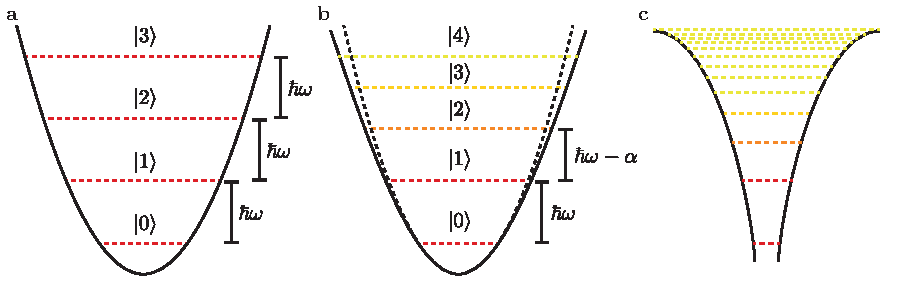
\includegraphics[width = 6in]{scqb_chapter/anharmonic_potential}
\end{center}
\caption[Harmonic and anharmonic potential energy and level spacing]{\textbf{a} Harmonic oscillator potential and energy levels, showing equal level spacing of $\hbar \omega$.  \textbf{b} Harmonic potential (dashed black line) with a softening correction (solid black line), showing decreasing energy level spacing by the anharmonicity parameter $\alpha$ with increasing energy level.  A stiffening potential would produce a positive anharmonicity rather than a negative one, increasing the frequency of higher level transitions.  \textbf{c} Rough schematic of the potential of a highly anharmonic system such as a hydrogen atom.  In general the anharmonicity in an atomic system is quite large as the potential is far removed from that of a harmonic oscillator; for the three lowest-lying states of the simple hydrogen atom, $E_{12} \approx 0.15 E_{01}$, a fractional anharmonicity of order unity.}
\label{fig:anh_pot}
\end{figure*}

The limitation of a harmonic oscillator as a controllable quantum system, as I mentioned in the previous section, is that any classical control field applied to the oscillator will produce a classical state of the oscillator.  The intrinsic reason for this is the equally spaced energy levels of the harmonic oscillator, illustrated in Figure \ref{fig:anh_pot}a.  A classical field will cause the ground state wave packet to climb the ladder, resulting in a coherent state consisting of a weighted superposition of every number state with some mean excitation number $\bar{n}$.  To prevent this from occurring, we must introduce some amplitude-dependent shift in the energy levels of the oscillator.  To make a mechanical analogy, we require the spring constant of the oscillator to either increase or decrease as a function of the displacement of the spring from equilibrium.  We will focus on a case where the spring constant decreases with increasing displacement, also known as a ``softening potential'' as the spring becomes less stiff with increasing displacement.

A softening potential is shown in Figure \ref{fig:anh_pot}b along with the first few energy levels.  At small amplitude, the potential is essentially quadratic, so the first level splitting $E_{01}$ remains unchanged as $\hbar \omega$.  The second level splitting $E_{12}$, however, is decreased by an amount $\alpha$, the \textit{anharmonicity}.  Higher level splittings are still further decreased.  The typical anharmonicity in the circuits described in this thesis is relatively small, on the order of 10\%.  This is in contrast to many anharmonic systems described in quantum mechanics, such as the hydrogen atom.  A cartoon of a atomic-type potential is shown in Figure \ref{fig:anh_pot}c, showing far more anharmonic level spacings than a simple softening potential.

For an anharmonic oscillator initially in the ground state, a coherent drive at frequency $\omega$ has the effect of driving Rabi oscillations between the first two states.  For a purely monochromatic excitation (or at least an excitation with bandwidth much smaller than the anharmonicity) the oscillator cannot climb out of the $\{|0\rangle,|1\rangle\}$ manifold.  We now have a system capable of demonstrating highly quantum behavior using only simple classical control fields.

\subsection{Superconducting anharmonic oscillators}

To realize an anharmonic LC oscillator we require a nonlinear circuit element.  There is no fundamental reason to prefer to make the capacitance or the inductance nonlinear, and classical electronics have utilized both as nonlinear elements.  To ensure that our oscillator behaves quantum-mechanically, however, we require a circuit element that is not only nonlinear but also nondissipative.  Conveniently, there is a circuit element unique to superconducting circuits that fits the bill: the \textit{Josephson tunnel junction} \cite{scqubitsrev2008}.  Physically, a Josephson junction is a thin non-superconducting (usually insulating) material sandwiched between two superconducting electrodes.  The insulating barrier must be thin enough that Cooper pairs can readily tunnel through the barrier.  When a supercurrent tunnels through the barrier it acquires a phase shift $\delta$ due to the first Josephson relation
\begin{equation}
I = I_0 \sin{\delta}
\label{eq:CPR}
\end{equation}
where $I_0$ is the \textit{critical current} of the junction, the maximum current that can flow through the junction without a finite voltage appearing across it.  For a time-varying signal, the second Josephson relation relates the voltage across the junction to the time evolution of the phase shift
\begin{equation}
V = \frac{\Phi_0}{2\pi} \dot{\delta}
\label{eq:2nd_JR}
\end{equation}
where $\Phi_0 = h/2e$ is the superconducting magnetic flux quantum \cite{tinkham2004introduction}.

\begin{figure*}
\begin{center}
	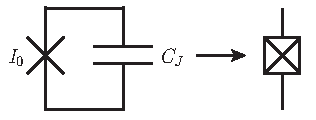
\includegraphics[width = 2.11in]{scqb_chapter/JJ_schem}
\end{center}
\caption[Josephson junction circuit schematic]{Circuit model for a Josephson junction including the intrinsic geometric parallel-plate capacitance.  The symbol at right is the circuit symbol for a junction including its intrinsic capacitance.}
\label{fig:JJ_schem}
\end{figure*}

From the definition of inductance $L = V/\dot{I}$ and equations (\ref{eq:CPR}) and (\ref{eq:2nd_JR}), we find that the impedance of the Josephson junction is that of an inductor whose value depends on the current flowing through it,
 \begin{equation}
L_J = \frac{\Phi_0}{2 \pi I_0 \cos{\delta}} = \frac{L_{J0}}{\sqrt{1 - I^2/I_0^2}}
\label{eq:LJ}
\end{equation}
where $L_{J0} = \Phi_0/2\pi I_0$ is the ``linear'' inductance of the junction for very small current.  For any physical Josephson junction, the thin metal-insulator-metal sandwich also forms an effective parallel-plate capacitor, usually modeled as an extra capacitance in parallel with the ideal Josephson element as shown in Figure \ref{fig:JJ_schem}.  Thus, a Josephson junction is itself intrinsically a nonlinear LC oscillator.  Due to the form of (\ref{eq:LJ}), the inductance of the junction increases with increasing current, and thus the resonant frequency of the Josephson nonlinear oscillator decreases.  For moderate excitations, this looks much like the softening potential drawn previously in Figure \ref{fig:anh_pot}b.

Because the critical current and the junction capacitance scale linearly with the area of the junction, the self-resonant frequency (also called the \textit{plasma frequency}) of the junction
\begin{equation}
\omega_J = \sqrt{\frac{2 \pi I_0}{\Phi_0 C}}
\label{eq:plas_freq}
\end{equation}
is fixed for a given junction fabrication process.  This frequency is typically many tens of gigahertz, and is usually reduced by adding an additional shunt capacitance in parallel with the junction to bring the plasma frequency down into the few gigahertz regime for convenience of operation.  The full form of the potential can be calculated by expressing the energy in the junction $U$ as the time integral of the voltage across the junction multiplied by the current.  Assuming zero initial energy at $t = - \infty$ and applying the Josephson relations, the junction energy can be calculated as \cite{slichterthesis}
\begin{equation}
U = E_J (1 - \cos{\delta})
\label{eq:E_J}
\end{equation}
where $E_J$ is the characteristic Josephson energy scale $E_J = \Phi_0 I_0/2\pi = \hbar I_0/2e$.  Thus, we see that the full potential is a cosine function with a characteristic scale determined by the junction critical current.

\subsection{Transmon qubits}

The circuit implementation of the anharmonic oscillator I described in the previous section is called a \textit{transmon} qubit \cite{Houck2009,transmontheory}.  This circuit design was created at Yale and has become the superconducting qubit of choice for many research efforts in the field, and for good reason.  The transmon is a straightforward device to design, fabricate, and control, and is conceptually easy to think about.  Furthermore, the transmon consistently achieves long coherence times in the 10 to 100 microsecond range \cite{PhysRevB.77.180502,Paik_3DT}, very long compared to 10 to 50 nanoseconds, the typical time required to do an arbitrary rotation of the qubit state \cite{PhysRevLett.102.090502}.

The circuit schematic for the transmon qubit is, remarkably, no different from that of a Josephson junction with intrinsic shunt capacitance; the main difference is the presence of an additional, large external shunting capacitance across the junction.  The purpose of this large capacitance is to reduce the single-electron charging energy associated with the total capacitance $E_C = e^2 / 2 C$.  This effectively flattens the dispersion of the energy eigenstates in the charge dimension, ensuring that the transmon qubit is essentially immune to dephasing due to charge noise.  To ensure the qubit is deep in this regime, we generally target $E_C$ to be about 1\% of $E_J$.  For an extensive theoretical discussion of the theory of the transmon, see reference \cite{transmontheory}.

The transition frequency between the two lowest energies of the transmon is approximately equal to the plasma frequency \eqref{eq:plas_freq}; re-expressing this in terms of $E_J$ and $E_C$ yields $\omega_{01} \approx \sqrt{8 E_J E_C}/\hbar$.  With the constraint $E_C \sim E_J/100$ and the requirement that the qubit frequency be experimentally convenient---say, 6 GHz---implies that $E_J \sim 3.5 \ \hbar \omega_{01} \sim h \times 20$ GHz, and thus $E_C \sim h \times 200$ MHz, with junction critical current $I_0 \sim 50$ nA and total capacitance $C \sim 100$ fF.  The primary limitation of the transmon qubit is the fact that the anharmonicity $\alpha$ is approximately $-E_C$, and thus the transition frequency $\omega_{12}$ is just a few percent lower than $\omega_{01}$.  To ensure that the transmon state remains in the $\{ \ket{0},\ket{1} \}$ manifold, the bandwidth of the control pulses used to induce qubit state transitions must be smaller than the anharmonicity \cite{PhysRevA.82.040305}.

\section{Cavity quantum electrodynamics}

With the transmon qubit in hand, we have a controllable, coherent quantum circuit with which we can perform experiments requiring a quantum two-level (or few-level) system.  However, we have not yet developed any description of how to couple these qubits to other quantum systems or to the outside world to enable the measurement of their quantum state.  In this section I will introduce the paradigm of \textit{cavity quantum electrodynamics} (cavity QED) \cite{bermanbook}, an approach which has been extremely fruitful in the study of real atoms \cite{RevModPhys.73.565,0034-4885-69-5-R02} and more recently quantum circuits \cite{cQEDtheory,blai07}.

\begin{figure*}
\begin{center}
	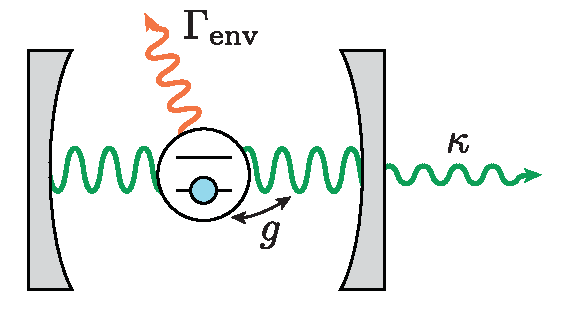
\includegraphics[width = 3.75in]{scqb_chapter/cav_QED}
\end{center}
\caption[Cavity QED schematic]{A simplified picture of a cavity QED setup.  An atom is placed inside a cavity resonator.  A particular transition of the atom is coupled to the standing mode inside the cavity with a coupling strength $g$.  The cavity filters the radiative density of states seen from the perspective of the atom, ideally reducing the atomic decay rate to the environment $\Gamma_{\rm env}$ to a negligible value.  One of the mirrors of the cavity is partially transmissive, allowing photons in the cavity mode to controllably leak out of the resonator at a rate $\kappa$.}
\label{fig:cav_QED}
\end{figure*}

A simplified picture of a cavity QED system is shown in Figure \ref{fig:cav_QED}.  The reasons for enveloping an atomic system of interest in a resonant cavity are several.  For atomic systems, perhaps most importantly, the presence of the cavity filters the radiative density of states seen by the atom.  A free excited atom in the continuum has a very large density of states to radiate into, and as a result atomic excited states tend to decay very quickly.  If the atomic transition of interest is tuned into resonance with the cavity, then the excited state will preferentially radiate into this mode.  However, because the resulting photon remains in the cavity for a long time, the atom has many opportunities to re-absorb it.  A more precise quantum picture of this process is simply that atomic excitation will be coherently exchanged with the resonator according to the coupling rate $g$.  If the coupling rate $g$ can be made much larger than the environmental decay rate $\Gamma_{\rm env}$ and the cavity decay rate $\kappa$, a cavity QED system can thus achieve strong coupling between a single atomic mode and a single photon, probing the most fundamental interaction diagrams in QED.

\subsection{Jaynes-Cummings Hamiltonian}

In the limit $\Gamma_{\rm env} \rightarrow 0$, and for now ignoring the cavity decay $\kappa$, a cavity QED system is described by the Hamiltonian \cite{wallbook}
\begin{align}
\label{eq:JC_H_terms} H & = H_q + H_r + H_{int} \\
& = \frac{1}{2}\hbar\omega_q\sigma_z + \hbar \omega_r a^{\dagger} a + \hbar g (a +a^{\dagger})(\sigma_+ + \sigma_-), 
\end{align}
where on the first line we have broken up the Hamiltonian into terms describing the free evolution of the qubit and resonator ($H_q$ and $H_r$, respectively) and their interaction ($H_{int}$), and $\omega_q$ is the transition frequency of the two-level atom, $\omega_r$ is the cavity resonant frequency, $a^{\dagger}$ and $a$ are the cavity creation and annihilation operators, and $\sigma_+$ and $\sigma_-$ are the qubit raising and lowering operators given by $(\sigma_x \pm i \sigma_y)/2$.  We can simplify this expression by ignoring the interaction terms that don't conserve excitation number (the ``rotating wave approximation''), resulting in the Jaynes-Cummings (JC) Hamiltonian
\begin{equation}
H_{JC} = \frac{1}{2}\hbar\omega_q\sigma_z + \hbar \omega_r a^\dagger a + \hbar g (a \sigma_+ +a^\dagger \sigma_-).
\label{eq:JC_H}
\end{equation}
The interaction term can now be interpreted in a straightforward manner as the exchange of an excitation between the atom and cavity.  The elegant simplicity of this Hamiltonian is one of the reasons for the remarkable success of cavity QED systems in implementing highly coherent control of single atomic quantum degrees of freedom.

\subsection{Circuit implementation of cavity quantum electrodynamics}

\begin{figure*}
\begin{center}
	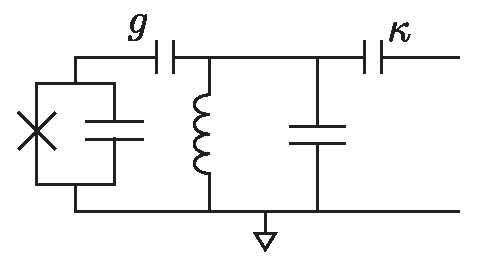
\includegraphics[width = 3.25in]{scqb_chapter/cQED}
\end{center}
\caption[Circuit QED schematic]{A circuit diagram which implements the same Hamiltonian as a cavity QED system.  A transmon qubit, at left, is capacitively coupled with strength $g$ to an LC resonator.  The resonator is capacitively coupled to the environment with rate $\kappa$.  It is also quite possible to replace one or both capacitive couplings with inductive couplings.  The circuit as drawn contains an explicit ground reference, though this is not necessary and cQED systems are often implemented as partially or fully differential circuits to reject common-mode interference.}
\label{fig:cQED}
\end{figure*}

I have already introduced all of the components necessary to realize an electrical circuit which is entirely analogous to a cavity QED system.  This paradigm is known as \textit{circuit QED} (cQED); a circuit schematic for such a system is shown in Figure \ref{fig:cQED}.  A superconducting transmon qubit plays the role of a single atom, and an electrical resonator plays the role of the cavity.  However, there are several important differences between atomic cavity QED and cQED.  Atomic systems are limited in the magnitude of $g$ by the size of the intrinsic dipole moment of the atomic transition of interest.  In circuit-based systems, $g$ can be adjusted independently of the other parameters by altering the size of the coupling capacitor, and schemes have even been demonstrated to dynamically tune this parameter on the same time scale as coherent qubit state rotations \cite{PhysRevB.84.184515}.

Additionally, circuits do not suffer from the intrinsic free-space radiative problem of real atoms, as they need not have any true geometric dipole moment.  Thus, for cQED systems, reduction of $\Gamma_{\rm env}$ is not a primary motivation for coupling the qubit to a cavity.  Furthermore, this also implies that the qubit need not be placed ``inside'' the cavity, permitting the use of flexible circuit topologies.  For cQED systems, the real reason for the cavity is to permit the non-invasive measurement of the qubit state, which is the subject of the next section.  In some multi-qubit experiments, several qubits are coupled to the same cavity which is then used as a ``quantum bus'' to allow the controllable coherent exchange of energy between the qubits \cite{Majer2007,Mariantoni2010}.

Although the system described so far is entirely composed of circuit elements, a experimentally practical hybrid system called the ''3D transmon'' architecture is commonly used as well \cite{Paik_3DT}.  The circuit comprising the transmon qubit is essentially the same, but rather than being capacitively-coupled to a circuit-style resonator, the qubit is coupled to a mode of a 3D waveguide cavity with a pair of large antenna paddles.  This architecture provides very long qubit coherence times by minimizing the interaction between the quantum modes of the qubit and any defects in the materials on which it is fabricated.  All of the experiments described in this thesis use this 3D transmon architecture.

\subsection{Dispersive regime and QND measurement}

Though the JC Hamiltonian generally describes the behavior of cQED systems for a large range of parameter regimes, the most relevant regime for the experiments described in this thesis is the so-called \textit{dispersive} regime, where the magnitude of the qubit-cavity detuning $\Delta = \omega_q - \omega_r$ is much larger than the coupling rate $g$.  Since excitations are quantized, in this regime the qubit and cavity cannot efficiently exchange energy with one another.  By expanding $H_{int}$ to second order in the small parameter $g/\Delta$ we find a revised interaction term
\begin{equation}
H_{int} =- \chi a^{\dagger} a \sigma_z
\end{equation}
where we've introduced the dispersive coupling rate $\chi = g^2 / \Delta$. Because $H_q \propto \sigma_z$ and $H_r \propto a^\dagger a$, the interaction term now commutes with the qubit and resonator terms, satisfying the requirement for a QND measurement (\ref{eq:QND_cond}).  This can be made more explicit by rewriting (\ref{eq:JC_H_terms}) with the dispersive interaction $H_{int}$ and re-grouping the terms as
\begin{equation}
H_{disp} = \frac{1}{2} \hbar \omega_q \sigma_z + \hbar \left(\omega_r + \chi \sigma_z \right)a^\dagger a.
\label{eq:Hdisp_qumeas}
\end{equation}
We can interpret the second term as the Hamiltonian of a quantum harmonic oscillator with a resonant frequency shifted by $\pm \chi$ depending on the qubit state operator $\sigma_z$.  Thus, a measurement which probes the resonant frequency of the cavity realizes a QND measurement of the state of the qubit.

Our choice of the grouping of the terms in (\ref{eq:Hdisp_qumeas}) was entirely arbitrary; we could have instead lumped the interaction term into $H_q$, realizing the Hamiltonian
\begin{equation}
H_{disp} = \frac{1}{2} \hbar (\omega_q + 2 \chi a^\dagger a)  \sigma_z + \hbar \omega_r a^\dagger a.
\label{eq:Hdisp_cavmeas}
\end{equation}
Now we can interpret the first term as a qubit whose transition frequency is shifted\footnote{This frequency shift can be interpreted as an incarnation of the AC Stark effect.} by $2 \chi$ times the photon number operator $a^\dagger a$, and thus a measurement which probes the transition frequency of the qubit realizes a QND measurement of the cavity photon number.  In reality, both of these effects occur simultaneously, and which form of the Hamiltonian we consider is largely a matter of convenience dictated by which quantity is measured in an experiment.  None of the experiments performed in this thesis involve the frequency-selective measurement of the qubit state, and thus I will focus the discussion to how measurement is performed within the context of (\ref{eq:Hdisp_qumeas}).

How is a measurement of the cavity frequency performed in practice?  A probe signal is injected into the cavity; this signal becomes entangled with the qubit state, and subsequently leaks out of the cavity at the rate $\kappa$.  A measurement of some property of this signal that differs for the two qubit states consumes the entanglement and delivers some information about that state.  Generally speaking, the signals used for measurement are coherent states, classically represented as a complex phasor $a e^{i \phi}$.   If the amplitude or phase of this vector differs between the two qubit states, a measurement of this quantity amounts to a measurement of the qubit state.  The details of this scheme depend on the parameter regime of the experimental realization.  For simplicity in this discussion I will only consider a cQED system measured in reflection \cite{Boissonneault2009,Girvin2014}, and I will also assume the cavity has no important internal losses.

\begin{figure*}
\begin{center}
	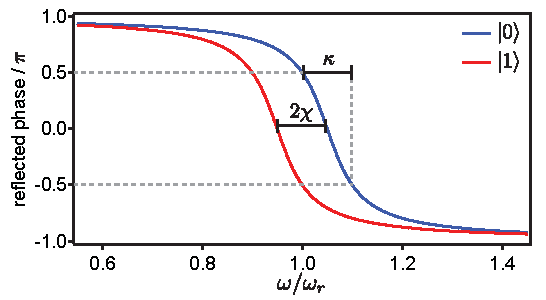
\includegraphics[width = 3.64in]{scqb_chapter/ref_phi}
\end{center}
\caption[Dispersive phase shift in reflection]{Reflected phase shift vs. normalized frequency for the case $2 \chi = \kappa$ where $\chi$ is negative.  Measuring the phase of a reflected probe signal at a frequency where the reflected phase differs constitutes a measurement of the state of the qubit.}
\label{fig:ref_phi}
\end{figure*}

When a cavity is measured in reflection, the probe signal acquires a frequency-dependent phase shift plotted in Figure \ref{fig:ref_phi}.  The total phase shift is zero at the resonant frequency $\omega_r$ and $\pm \pi$ at large detunings.  If the qubit is in the $\ket{0}$ ($\ket{1}$) state, the cavity resonance is shifted by $-\chi$ ($+\chi$).  Thus, a measurement signal at an intermediate frequency acquires a different reflected phase for the two states.  Whether or not this measurement constitutes a projective or partial measurement of the state depends on a variety of system parameters, including the magnitude of the coherent state $\bar{n}$, the amount of time the output signal is integrated for, and the magnitude of the phase shift.  For the case of a transmission measurement the picture is essentially the same, though the phase shift is reduced by a factor of 2 and the two signals will have a difference in amplitude as well as phase if the measurement frequency is not at exactly $\omega_r$.

\begin{figure*}
\begin{center}
	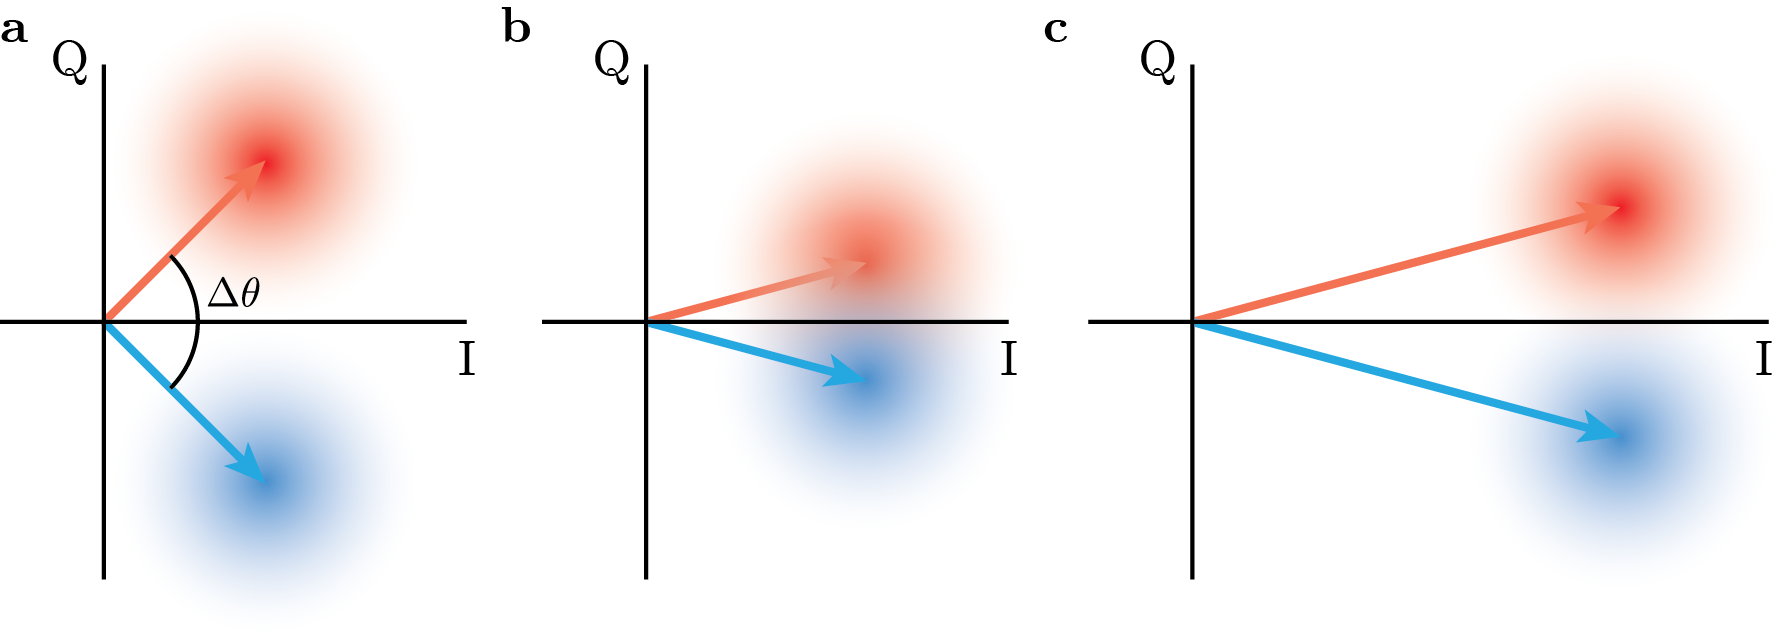
\includegraphics[width = 6in]{scqb_chapter/IQ_blobs.png}
\end{center}
\caption[IQ histograms for various parameters]{Simulated histograms for qubit-state-dependent IQ shifts.  The finite spatial extent of the histograms is due to quantum and classical noise in the two quadratures of the field.  \textbf{a} Well-separated histograms for $\Delta \theta = \pi/2$.  \textbf{b} Significantly overlapping histograms for the same coherent state amplitude, but with $\Delta \theta = \pi/6$.  \textbf{c} Increased histogram separation can be achieved for small phase shifts by increasing the coherent state amplitude.}
\label{fig:IQ_blobs}
\end{figure*}

For a single set of measurement parameters, we can qualitatively determine the strength of the measurement by plotting histograms of the measurement outcomes for the different qubit states in terms of the two cartesian coordinates (real and imaginary) which make up the complex phasor.  In the language of microwave electronics, these two coordinates are called the \textit{in-phase} and \textit{quadrature} components of the signal, or I and Q.  These histograms are depicted in Figure \ref{fig:IQ_blobs}.  For a single measurement, if the histograms are well-separated as in Figure \ref{fig:IQ_blobs}a, this constitutes a projective measurement of the qubit state (corresponding to Figure \ref{fig:ideal_proj_meas}).  If the histograms are significantly overlapping, we realize a partial measurement of the qubit state (corresponding to Figure \ref{fig:ideal_partial_meas}).  Keeping all other parameters fixed, we can increase the histogram separation by increasing the length of the coherent state vector.  However, there are practical limits to the maximum signal which can be utilized in a dispersive cQED measurement.  The dispersive approximation itself supplies a rough upper limit, as the validity of the dispersive approximation relies on the condition $\bar{n} < \bar{n}_{\textrm{crit}} = \Delta^2/4g^2$ \cite{slichterthesis}.  In practice this is not a hard limit, and relatively high-quality qubit readout has been performed with $\bar{n} \sim 3 \bar{n}_{\textrm{crit}}$ or so \cite{Jeffrey2014}.  At these large photon numbers, the measurement is typically no longer perfectly QND, but for short measurement times the error rate can be negligibly small.

It is important to note that because the transmon is only a weakly anharmonic system, the higher level transitions will also couple to the cavity mode, which significantly complicates the simple picture of a two-level system coupled to the cavity with a strength $g$.  The dispersive shift $\chi$ is no longer simply given as $g^2/\Delta$, but will rather be a sum over all of the coupling strengths $g_{ij}$ for the various state transitions $\omega_{ij}$.  For the experiments conducted in this thesis, this additional complexity can be entirely absorbed as a rescaling of the circuit QED parameters; in general the coupling strength $g$ is not directly important, and the dispersive shift $\chi_{01}$ due to the first level transition is directly measured in experiment anyway.  For a full treatment of the multi-level transmon in circuit QED, see references \cite{slichterthesis,Weber2014a}.

\subsection{Back-action of cQED measurement}\label{s:cQED_backaction}

Most of the results in this thesis were made with cQED systems in the dispersive weak measurement limit.  As discussed previously, the strength of a measurement depends not only on the fixed system parameters but also on the signal magnitude used in the measurement; thus, a vast range of measurement strengths can be accessed in a single apparatus.  However, the fixed system parameters result in a intrinsic scale of measurement strength corresponding to the state-dependent phase shift $\Delta \theta = 2 \tan^{-1}(2 \chi / \kappa)$, and several equations of interest take on a relatively intuitive and simple form in the limit $\Delta \theta \ll 1$.

To elucidate some of the interesting and unintuitive details of the back-action of the cQED measurement, I will follow the very good discussion in reference \cite{koro11}.  For a cQED setup in the dispersive limit with $\omega = \omega_r$, the ensemble dephasing due to the presence of a measurement coherent state with mean photon number $\bar{n}$ is given by
\begin{equation}
\Gamma = \frac{8 \chi^2 \bar{n}}{\kappa}.
\label{eq:cQED_dephasing}
\end{equation}
This coherent state corresponds to the oscillation of the field expectation value $\xpec{F(t)} = 2 \sqrt{\bar{n}} \sigma_{\rm gr} \cos(\omega t)$, where $\sigma_{\rm gr}$ is the ground state amplitude width due to quantum fluctuations which here serves to re-scale the coherent state amplitude into ``uncertainty units'' (note that $\sigma_{\rm gr} = 1/4$).  Interaction with the qubit then creates a phase shift of $\pm 2 \chi/\kappa$ depending on the qubit state.  Decomposing the resulting phasor into quadrature components results in
\begin{gather}
\xpec{F(t)} = \rm I \cos(\omega t) + \rm Q \sin(\omega t) \notag \\
\rm I = 2 \sqrt{\bar{n}} \sigma_{\rm gr} \quad \rm Q = 2 \sqrt{\bar{n}} \sigma_{\rm gr} (2 \chi / \kappa) \xpec{\sigma_z}
\end{gather}
We can now explicitly see the information contained in each quadrature.  The large I quadrature contains information about the photon number fluctuations in the resonator, while the small Q quadrature contains information about the qubit state.  If we use an interferometric apparatus to selectively measure only the Q quadrature (this will be a phase-sensitive parametric amplifier; see section \ref{s:phase_sens_amps}), by emptying the resonator of its contents we can measure the Q quadrature with imprecision $\sigma_{\rm gr}$.  In the limit of a continuous-time measurement, we achieve an imprecision in Q of $\sigma_{\rm gr} / \sqrt{\kappa t}$, or, equivalently, an imprecision in $\xpec{\sigma_z}$ of $\sqrt{\kappa/t}/(4 \chi \sqrt{\bar{n}})$.  Linking back to the discussion in section \ref{s:bayesian}, the full swing of our detector between $\sigma_z = \pm 1$ is thus
\begin{equation}
\Delta V = 8 (\chi/\kappa) \sqrt{\bar{n}} \sigma_{\rm gr},
\end{equation}
and the imprecision $\sigma$ in the output signal $V(t)$ is
\begin{equation}
\sigma = \sqrt{\frac{\kappa}{t}} \left( \frac{\Delta V}{8 \chi \sqrt{\bar{n}}} \right).
\end{equation}
Thus, we can express the power spectral density of the output noise as
\begin{equation}
S = 2 t \sigma^2 = \frac{ (\Delta V)^2 \kappa}{32 \chi^2 \bar{n}}.
\end{equation}
From \eqref{eq:bayesian_dephasing}, we calculate the dephasing rate associated with this measurement as
\begin{equation}
\Gamma = \frac{(\Delta V)^2}{4S} = \frac{8 \chi^2 \bar{n}}{\kappa}.
\end{equation}

This is an important result; because the dephasing rate associated with measuring only the Q quadrature of the output signal accounts for all of the ensemble qubit state dephasing, this measurement process can have no back-action besides the Bayesian evolution described in section \ref{s:bayesian}.  Thus, the only back-action of this measurement process is the stochastic evolution of the Bloch vector towards one of the poles, with no accompanying evolution in the phase of an initial superposition.  In other words, if the Bloch vector begins on a particular meridian of the Bloch sphere, the action of the measurement is to drive stochastic evolution of the state vector along this meridian only.

What if we were to instead measure the I quadrature?  For a measurement time $t$, we measure I with an imprecision $\sigma_{\rm gr} / \sqrt{\kappa t}$, which can be understood as a measurement of the fluctuation of the number $N$ of emitted photons in that time $\mathrm{var}(N) = \bar{n}\kappa t$, which follows from the fact that the variance of the photon number in a coherent state is equal to the mean photon number $\bar{n}$, the photons are leaking from the cavity at the rate $\kappa$, and we capture them for a time $t$.  Because the correlation function of photon number in the resonator depends on time as $\exp(-\kappa t/2)$ \cite{clerk_revmod}, the effect of detecting an amplitude fluctuation corresponding to one photon\footnote{Because our detector output is a continuous field variable and not a photon-counting detector, thinking of the output field in terms of individual photon detection events is not formally correct, but the intuition it provides is essentially correct if we're careful about factors of 2.} implies that that fluctuation on average spent a time $2/\kappa$ in the resonator (this is the lifetime of the field amplitude; the power of course has the lifetime $1/\kappa$), resulting in an evolution of the qubit phase by $4\chi/\kappa$.  Thus, the variance in the qubit phase is $\mathrm{var}(\phi) = (4 \chi/\kappa)^2 \bar{n}\kappa t$, implying a dephasing rate $\Gamma = \mathrm{var}(\phi) / 2 t = 8\chi^2 \bar{n} / \kappa$.  We have once again recovered the standard result for the total ensemble dephasing, implying that the resulting ``pure dephasing'' associated with measuring the I quadrature represents the entire back-action of the measurement.

What if we were to measure both the I and Q quadratures simultaneously?  The measurement simultaneously acquires information about both the qubit state and the photon number fluctuations, and both kinds of back-action occur simultaneously.  It turns out (see section \ref{s:phase_pres_amps}) that due to the field commutation relations, an ideal measurement of both quadratures implies doubling the size of the uncertainty compared to the single-quadrature case.  Because the power spectral density of the noise has been increased by a factor of two, the dephasing rate for each back-action process is reduced by a factor of two, both then contributing an equal half of the total dephasing rate $\Gamma$ in \eqref{eq:cQED_dephasing}.  An in-depth discussion of how both single-quadrature and two-quadrature measurements are made in practice is the subject of the next chapter.

































\chapter{Quantum-limited amplifiers}
\label{c:paramps}

Thus far, I have discussed idealized quantum measurements, and the paradigm of circuit QED in which we can in practice realize coupled quantum systems which implement these measurements.  What I have not yet discussed, however, is how we build the bridge from this quantum world to the classical world in which we interpret our experimental outcomes.  In general, quantum measurements at some point involve one or more stages of \textit{signal amplification}.  This is necessary because the energy and power scales of quantum systems are usually much, much smaller than the energy and power scales of our classical experimental apparatus.  To bridge this gap, we must create some highly sensitive nonlinear coupling between the quantum degree of freedom and a classical degree of freedom.  A classic example of such a coupling is a photomultiplier tube, a device capable of measuring the arrival time and energy of a single optical photon to high precision.  The arrival of a photon creates an ionization event which cascades down a series of metal plates biased with very high voltage, resulting in a very large current pulse.  Considering that the initial photo-ionization event produces a single electron, the total current pulse is equivalent to a signal gain of 70 dB or more \cite{Hakamata2002}.

In the context of superconducting circuits, most all signals are continuous-value microwave fields, usually Gaussian coherent states.  The signal powers are typically quite weak: the resonant frequency and bandwidth of a typical circuit QED cavity are on the other of 5 GHz and 5 MHz, respectively, and the cavity is typically driven with a intracavity field corresponding to a mean cavity occupation $\bar{n}$ on the order of 1 or so.  This corresponds to an output power of $P = \hbar \omega \kappa \bar{n} \sim 1 \times 10^{-16}$ W $ = -130$ dBm.  The typical powers used in analog microwave signal processing in the classical regime at room temperature are on the order of $10^{-3}$ W $= 0$ dBm, so we require about 13 orders of magnitude of amplification to bridge these disparate scales.  However, unlike for destructively detecting the incidence of a single optical photon, we require this amplification to produce a faithfully amplified copy of the continuous-valued input signal while adding as little noise to this signal as possible.  This type of amplification is usually called \textit{linear amplification}, as the output signal $V_{\textrm{out}}(t)$ should obey the relation
\begin{equation}
V_{\textrm{out}}(t) = \sqrt{G} V_{\textrm{in}}(t) + \epsilon(t)
\label{eq:lin_amp}
\end{equation}
where $G$ is the real-valued amplifier power gain, $V_{\textrm{in}}(t)$ is the input signal, and $\epsilon(t)$ is additional uncorrelated noise added by the amplification process.

\section{Amplifier figures of merit}\label{s:amp_figures_of_merit}

\begin{figure*}
\begin{center}
	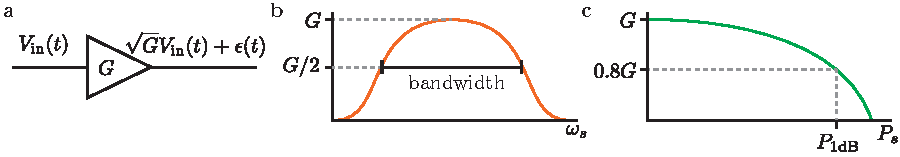
\includegraphics[width = 6in]{paramps_chapter/amp_metrics}
\end{center}
\caption[Amplifier performance metrics]{\textbf{a} A generic amplifier, characterized by its power gain $G$.  The amplifier output contains an amplified copy of the signal as well as some additional noise $\epsilon(t)$.  \textbf{b} The bandwidth of an amplifier is commonly defined as the frequency band over which the amplifier delivers a gain at least as large as $G/2$.  \textbf{c} The input signal power at which the gain is reduced to approximately 80\% (-1 dB) of the small-signal gain is a common figure of merit for amplifier input power handling ability, called the 1 dB input compression power or $P_\textrm{1dB}$.}
\label{fig:amp_metrics}
\end{figure*}

There are several parameters of interest in characterizing the performance of a generic linear amplifier, illustrated in Figure \ref{fig:amp_metrics}.  Ideally, the amplifier faithfully creates an amplified copy of the input signal, increasing the power of that signal by a factor of the power gain $G$.  In the process of amplification, the amplifier also adds some extra noise to the output signal $\epsilon(t)$.  We usually make the approximation that this added noise is independent of the input signal, uncorrelated with itself (white noise), and Gaussian-distributed.  This is a good approximation for thermal noise sources such as Johnson noise and also describes the character of the quantum vacuum noise \cite{clerk_revmod}.

We express this noise in power units over some reference bandwidth $B$, usually taken to be 1 Hz.  We can use Boltzmann's constant $k$  to convert the resulting power into a \textit{noise temperature}
\begin{equation}
T_N = \frac{P_N}{B k}.
\label{eq:Tnoise}
\end{equation}
The output noise temperature of an amplifier is usually \textit{referred} to the input of the amplifier by dividing the output noise temperature by $G$, permitting a straightforward comparison to any relevant noise scales in the input signal.  In general we wish for the input noise of an amplifier to be much smaller than the input signal, permitting a faithful recovery of the input signal from the output.  An extensive discussion of how to measure the noise temperature of a cryogenic amplifier is given in \cite{slichterthesis}.  I will also describe a high-precision technique for making this measurement in chapter \ref{c:twpa_exp}.

The dynamics and amplification mechanism of an amplifier usually provide linear operation only over some finite range of signal frequencies, the \textit{bandwidth} of the amplifier.  Defining bandwidth is somewhat arbitrary, but a commonly-used metric is the frequency band over which the amplifier produces gain at least as large as half of the peak gain, as depicted in Figure \ref{fig:amp_metrics}b.  For gain profiles that are more complex that a simple hump, this definition may not make sense, but it is generally applicable to the amplifiers discussed in this thesis.

Finally, because any amplifier has a finite reservoir of energy to use for amplification, if an input signal becomes too large, the amplifier may not be able to faithfully reproduce it.  This is called \textit{input compression}, and is depicted in Figure \ref{fig:amp_metrics}c.  Generally, when an amplifier becomes compressed, it is no longer able to deliver the full gain $G$ but instead the effective gain starts to decrease as a function of increasing input signal power.  The standard metric for input compression is the input signal power at which the gain of the amplifier is reduced by 1 dB (to approximately $0.8G$), and is the metric discussed in the remainder of this thesis.



\section{Quantum limits on amplification}

Amplification is essentially a form of measurement, as an amplifier is a device that interacts with an input signal and produces an output signal which is correlated with the input signal.  It should be obvious that we wish to minimize the term $\epsilon(t)$ in (\ref{eq:lin_amp}), as this added amplifier noise distorts the output signal and prevents us from recovering the exact input signal.  Considering that quantum mechanics places intrinsic lower bounds on the uncertainty of making various types of measurements, it should come as no surprise that amplification must satisfy some minimum uncertainty relation which constraints just how faithfully the output signal of the amplifier can correlate with the input signal.  The seminal work on deriving a general quantum limit for a linear amplification process was done by Caves in reference \cite{Caves1982a}, though earlier work dates back to 1962 \cite{PhysRev.128.2407,4066904}.  In this section,
 I will follow a more modern review of the subject which I find somewhat more illuminating \cite{clerk_revmod}.

For a continuous, narrowband classical signal $V(t)$ centered at frequency $\omega$, we can write $V(t)$ in terms of a complex number $a$, defining the amplitude and phase of the signal
\begin{equation}
V(t) \propto i ( a e^{-i \omega t} - a^* e^{+i \omega t} ).
\end{equation}
Since we are concerned with the quantum properties of this signal, we must promote $a,a^*$ to the level of quantum ladder operators $a \rightarrow \hat{a}$, $a^* \rightarrow \hat{a}^\dagger$.  For simplicity I'll not bother with the hats for the remainder of the section.  Equivalently, we could instead use the two quadrature amplitude operators I and Q, with functional form
\begin{equation}
\mathrm{I} = \frac{1}{\sqrt{2}} (a^\dagger + a) \quad \mathrm{Q} = \frac{i}{\sqrt{2}} (a^\dagger - a)
\end{equation}
with the commutation relation $[\mathrm{I}, \mathrm{Q}] = i$.  Since the field quadratures are canonically conjugate quantities, we cannot expect to be able to measure both simultaneously to arbitrary precision.

\subsection{Phase-preserving amplification}\label{s:phase_pres_amps}

\begin{figure*}
\begin{center}
	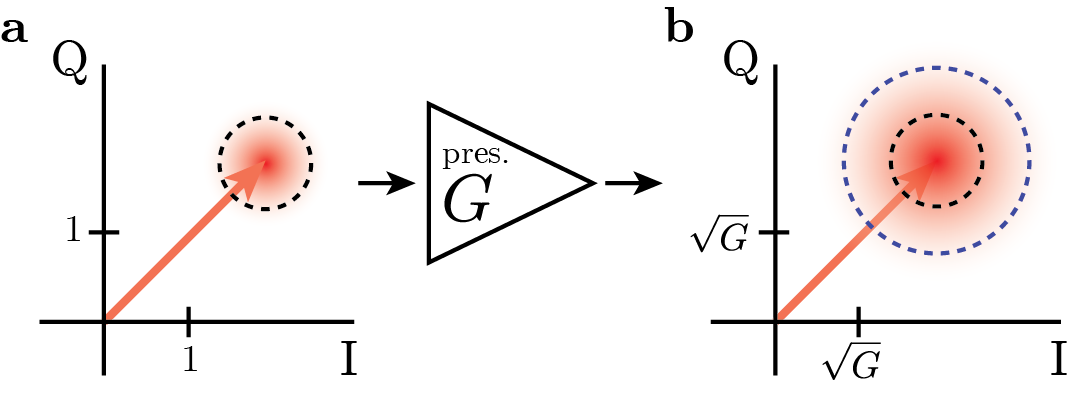
\includegraphics[width = 3.75in]{paramps_chapter/lollipops_pres.png}
\end{center}
\caption[IQ diagram for phase-preserving amplifier]{\textbf{a} IQ diagram of an input coherent state vector, including an uncertainty ``blob'' at the end of the vector representing the vacuum fluctuations.  \textbf{b} The output state, following amplification by a phase-preserving amplifier with gain $G$ (note axis rescaling).  The action of the amplifier has amplified the input vector while maintaining the phase, but has also added some extra noise (dashed purple circle) onto the noise present at the input (black dashed circle).}
\label{fig:lollipops_pres}
\end{figure*}

An amplifier which linearly amplifies both quadratures of the input signal is known as a \textit{phase-preserving} (or \textit{phase-insensitive}) amplifier, as the amplified copy of the signal preserves the phase of the input signal (or, equivalently, the amplification process is insensitive to the phase of the input signal and thus treats both quadratures equally).  A IQ diagram of the action of such an amplifier is shown in Figure \ref{fig:lollipops_pres}.

We consider first the case where an amplifier has just one mode at the input, $a_{\rm in}$, and one at the output, $a_{\rm out}$.  In the usual way, we define the uncertainty in the input field as
\begin{equation}
(\Delta a_{\rm in})^2 \equiv \frac{1}{2} \langle \{a_{\rm in},a_{\rm in}^\dagger \} \rangle - | \langle a_{\rm in} \rangle |^2
\label{eq:gen_uncert}
\end{equation}
with an analogous definition for $(\Delta a_{\rm out})^2$, where the curly brackets $\{~,\}$ indicate anticommutation.  The input and output operators must obey the usual bosonic commutation relations
\begin{equation}
[a_{\rm in},a_{\rm in}^\dagger] = 1, \quad [a_{\rm out},a_{\rm out}^\dagger] = 1.
\label{eq:quad_comm}
\end{equation}
We are seeking a faithful linear relationship between the input and output fields, thus implying that
\begin{equation}
a_{\rm out} = \sqrt{G} a_{\rm in}, \quad a_{\rm out}^\dagger = \sqrt{G} a_{\rm in}^\dagger.
\label{eq:dumb_linear}
\end{equation}
However, it is immediately clear that we cannot simultaneously satisfy (\ref{eq:quad_comm}) and (\ref{eq:dumb_linear}), so the simple linear relationship in (\ref{eq:dumb_linear}) cannot be correct.  We are thus forced to write
\begin{equation}
a_{\rm out} = \sqrt{G} a_{\rm in} + \mathcal{F}, \quad a_{\rm out}^\dagger = \sqrt{G} a_{\rm in}^\dagger + \mathcal{F}^\dagger.
\label{eq:linear_wF}
\end{equation}
What does $\mathcal{F}$ represent, physically speaking?  It cannot be correlated with $a$, else we would violate the commutation relation (\ref{eq:quad_comm}).  Thus we conclude that $\mathcal{F}$ must represent extra noise added by the amplifier.  What is the physical source of this noise?  Since the amplifier provides a power gain $G$, the energy needed to increase the signal power by $G$ must come from \textit{somewhere}, so these extra fluctuations represented by $\mathcal{F}$ are associated with this reservoir of power.

Since $\mathcal{F}$ is uncorrelated with the input signal mode $a_{\rm in}$, $[\mathcal{F},a_{\rm in}] = [\mathcal{F},a_{\rm in}^\dagger] = 0$ and $\langle F a_{\rm in} \rangle = \langle F a_{\rm in}^\dagger \rangle = 0$.  By enforcing the commutation relation (\ref{eq:quad_comm}) for the output field $a_{\rm out}$, we find that
\begin{equation}
[\mathcal{F},\mathcal{F}^\dagger] = 1 - G.
\label{eq:F_comm}
\end{equation}
What does this say about $(\Delta a_{\rm out})^2$, the noise in the output field?  Combining (\ref{eq:gen_uncert}) and (\ref{eq:linear_wF}),
\begin{align}
(\Delta a_{\rm out})^2 &= G (\Delta a_{\rm in})^2 + (1/2) \langle \{ \mathcal{F},\mathcal{F}^\dagger \} \rangle \notag \\
&\geq G(\Delta a_{\rm in})^2 + (1/2) \langle [ \mathcal{F},\mathcal{F}^\dagger ] \rangle  \notag \\
&\geq G(\Delta a_{\rm in})^2 + | G - 1|/2.
\label{eq:output_noise}
\end{align}
In the limit of no gain ($G = 1$), $(\Delta a_{\rm out})^2 = (\Delta a_{\rm in})^2$, and the amplifier need not add any noise.  However, for any gain larger than unity, the output noise must be strictly larger than the amplified input noise.  It is somewhat more illuminating to express this output noise on the same scale as the input noise:
\begin{equation}
(\Delta a_{\rm out})^2 / G \geq (\Delta a_{\rm in})^2 + |1 - 1/G|/2.
\label{eq:output_noise_input_ref}
\end{equation}
It is clear that in the case where $G \gg 1$, the final term will be very small, and so we make the approximation $G \rightarrow \infty$ and find a standard and beautiful result in quantum amplification:
\begin{equation}
(\Delta a_{\rm out})^2 / G \geq (\Delta a_{\rm in})^2 + 1/2.
\label{eq:half_quantum}
\end{equation}
Since we are working in units of photon number, the interpretation of this equation is straightforward.  Much as the ground state of the electromagnetic field intrinsically fluctuates at the level of half a quantum, a general phase-preserving amplifier in the large gain limit must necessarily add fluctuations at the level of half a quantum to the input.

We can go a bit further in understanding this added noise by finding a more detailed form for the extra noise operator $\mathcal{F}$.  From (\ref{eq:F_comm}), we see that for any $G > 1$ the RHS is negative.  If we introduce one additional bosonic mode $d$, corresponding to a mode from which we draw the energy needed for amplification, we can express the extra noise operator as
\begin{equation}
\mathcal{F} = \sqrt{G-1}d^\dagger, \quad \mathcal{F}^\dagger = \sqrt{G-1}d.
\end{equation}
This expression satisfies (\ref{eq:output_noise_input_ref}) as an equality, so an amplifier that realizes this type of operation could potentially add only the minimum half-quantum of noise at high gain.  With this definition for $\mathcal{F}$, we can write the amplifier scattering relation \eqref{eq:linear_wF} as
\begin{equation}
a_{\rm out} = \sqrt{G} a_{\rm in} + \sqrt{G-1} d^\dagger.
\end{equation}

\subsection{Phase-sensitive amplifiers}\label{s:phase_sens_amps}

\begin{figure*}
\begin{center}
	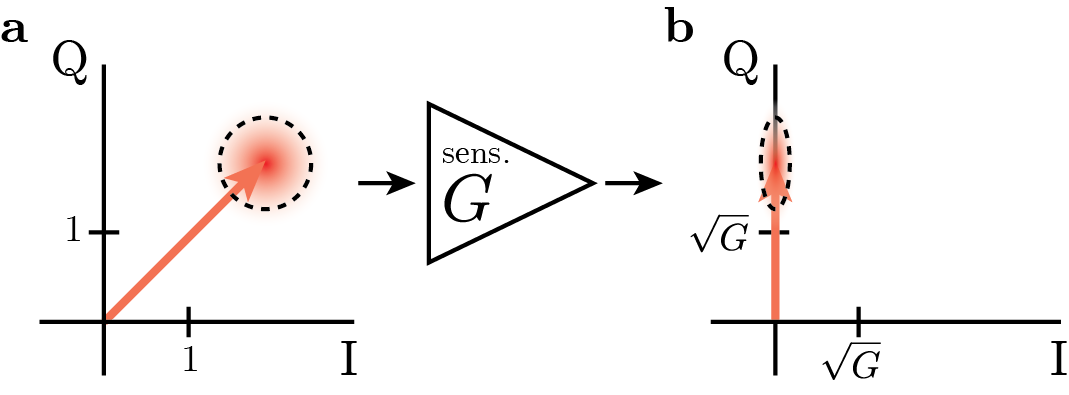
\includegraphics[width = 3.75in]{paramps_chapter/lollipops_sens.png}
\end{center}
\caption[IQ diagram for phase-sensitive amplifier]{\textbf{a} IQ diagram of an input coherent state vector, including an uncertainty ``blob'' at the end of the vector representing the vacuum fluctuations.  \textbf{b} The output state, following amplification by a phase-sensitive amplifier with gain $G$ aligned with the Q quadrature (note axis rescaling).  The action of the amplifier has amplified the input vector along the Q quadrature while de-amplifying the I quadrature.  The resulting ``squeezing'' of the noise is visible in the shape of the noise blob, which has been stretched along Q by $\sqrt{G}$ and compressed along I by $1/\sqrt{G}$; this compression along I implies the translation of the output state vector to the Q axis.}
\label{fig:lollipops_sens}
\end{figure*}

The extra half-quantum of input noise for a phase-preserving amplifier fundamentally arose from our assertion that the amplifier should linearly amplify both quadratures of the signal.  Since these two quadratures do not commute, we could not simultaneously satisfy the commutation relation and the naive requirement of linear amplification.  However, if we relax the linear amplification requirement and limit ourselves to amplifying only one input quadrature, say, the Q quadrature,
\begin{equation}
\mathrm{Q}_{\rm out} = \sqrt{G} \mathrm{Q}_{\rm in}, \quad \mathrm{I}_{\rm out} = \mathrm{I}_{\rm in} / \sqrt{G},
\label{eq:phase_sens}
\end{equation}
then the output fields clearly satisfy the commutation relation.

An amplifier that has an action of this form is known as a \textit{phase-sensitive} (or \textit{phase-nonpreserving}) amplifier, as the amplification process is different depending on the phase of the input signal (or, equivalently, the amplification process does not preserve the input phase of the signal).  Physically speaking, for the action of the amplifier to be different depending on the input phase of the signal implies that the input signal mode and the mode used to supply amplification energy must have a fixed phase relationship.  Here we now speak of $\rm Q$ as the \textit{amplified} quadrature and $\rm I$ as the \textit{deamplified} (or \textit{squeezed}) quadrature.  If the input mode $a$ is a vacuum state, $\rm Q_{out}$ will have fluctuations $\sqrt{G}$ times larger than the vacuum fluctuations, while $\rm I_{out}$ will have fluctuations $\sqrt{G}$ times \textit{smaller} than the vacuum!  This is shown schematically in the IQ plane in Figure \ref{fig:lollipops_sens}.

These are fundamentally quantum states of light, as they require correlations between signal components larger than the limits imposed by classical physics \cite{Loudon1987}.  Because \eqref{eq:phase_sens} satisfies the field quadrature commutation relation, a phase-sensitive amplifier need not intrinsically add any additional noise to the input signal.  In other words, because we are only measuring one half of a pair of non-commuting observables, there is no fundamental limit to how well we can measure that observable, so no added noise term need appear to satisfy such a limit.

\subsection{Quantum efficiency of phase-preserving amplifiers}

The result that a linear phase-preserving amplifier must add an additional half-quantum of noise has led to a great deal of confusion and misunderstanding about the quantum measurement performance of these types of devices.  Since the intrinsic fluctuations of the input mode $a$ correspond to half a quantum, the quantum limit of measuring this mode is often expressed as this same half-quantum.  Thus, if we consider the total input-referred noise of a phase-preserving amplifier to be this half-quantum plus an additional half-quantum, at face value it appears as if a phase-preserving amplifier is forever limited to operating with a quantum efficiency of 0.5.  However, this amounts to a fundamental misunderstanding of the quantum measurement process.

This understanding would be correct if we should place the added half-quantum of noise on the same footing as additional, uncorrelated classical noise in the measurement system.  However, this interpretation is not correct, and can be understood in terms of environmental correlations.  Classical noise $\epsilon(t)$ added by the measurement system is intrinsically part of the incoherent, dissipative classical environment associated with the imperfect measurement apparatus.  If we had perfect control over all of this environment, we could keep track of the exact form of this noise and simply subtract it from the output signal to perfectly recover the underlying signal plus quantum noise.  Thus, any additional classical noise that we do not have an independent record of spoils our perfect quantum-limited measurement.

\begin{figure*}
\begin{center}
	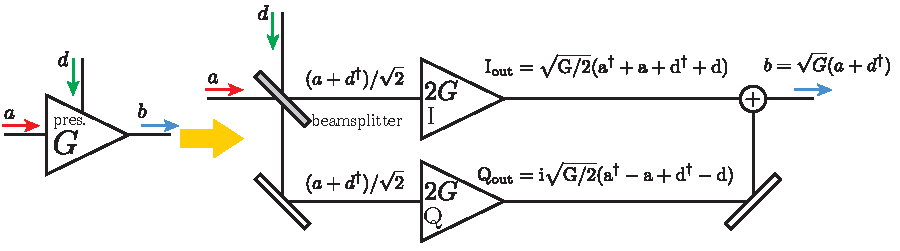
\includegraphics[width = 6in]{paramps_chapter/pres_from_sens}
\end{center}
\caption[Phase-preserving amplifier as two phase-sensitive amplifiers]{A schematic representation of how to create a phase-preserving amplifier with gain $G$ as the combination of two phase-sensitive amplifiers with gain $2G$ and one beam splitter.  We can physically understand the origin of the extra half-quantum of noise in this type of phase-preserving amplifier as the result of adding the second port on the beamsplitter, introducing another vacuum mode $d$.  Note that I have employed the large-gain limit to set $\sqrt{G-1} = \sqrt{G}$ and eliminate the squeezed quadratures from the outputs of the phase-sensitive amplifiers.}
\label{fig:pres_from_sens}
\end{figure*}

The extra minimum noise fundamentally associated with the extra mode needed in a phase-preserving amplifier, however, is not of this form.  Ideally, there is no record of these fluctuations imprinted in an environment beyond our control, so this noise is \textit{fundamentally indistinguishable} from the intrinsic quantum noise of the input mode.  Thus, these added fluctuations do not spoil the efficiency of our measurement.  We can loosely define the measurement efficiency $\eta$ as
\begin{equation}
\eta = \frac{\textrm{the information we collect}}{\textrm{the information we collect } + \textrm{ the information we lost}}.
\label{eq:eta_heur}
\end{equation}
Since the added quantum fluctuations in the extra mode are not correlated with any unmeasured degrees of freedom, we have not lost any information, and a perfect phase-preserving amplifier still has a quantum efficiency of unity once the quantum limit is correctly defined.

This idea can be made more clear by introducing a simple model for a phase-preserving amplifier by combining two phase-sensitive amplifiers, as shown in Figure \ref{fig:pres_from_sens}.  It is clear in this setup that at no point do we lose any information from the mode $a$, nor do we introduce any extra uncorrelated classical noise.  The only difference is the introduction of a beam splitter, adding an extra vacuum port through which the mode $d$ enters the system.  One way to understand the effect of the extra input vacuum mode is that the additional half-quantum of noise does not decrease the efficiency of the measurement, but merely reduces the \textit{strength} of that measurement by a factor of two.  Note that we have had to employ phase-sensitive amplifiers with gain $2G$ to model a phase-preserving amplifier of gain $G$.  This implies that regardless of which type of amplifier we use, we will still achieve quantum-limited measurement back-action as described in section \ref{s:cQED_backaction}.

\section{Practical ultra-low-noise microwave-frequency amplifiers}

Realizing microwave-frequency amplifiers that saturate these lower bounds on added noise is a very nontrivial task.  The input signals are very weak, and, moreover, the energy corresponding to the vacuum fluctuations at the input of the amplifier is extremely small.  We can use Boltzmann's constant to convert the characteristic energy scale of the vacuum fluctuations to a noise temperature $T = \hbar \omega / 2 k = 144$ mK at 6 GHz.  For the fields to be in their ground state, the thermal temperature of the environment must be about an order of magnitude lower than this still, implying an amplifier capable of operating at temperatures of a few tens of millikelvin.

The general design approach for building low-noise microwave amplifiers for operation at cryogenic temperatures utilizes high-quality microwave-frequency semiconductor transistors \cite{Wadefalk2003} made from high-electron-mobility transistors (HEMTs).  HEMT amplifiers are capable of operation at temperatures as low as a few kelvin, and the best devices achieve input-referred noise temperatures as low as 2 or 3 K.  This is still about an order of magnitude larger than the quantum limit!  We therefore need a different type of amplifier entirely, capable of operating at temperatures much lower than the quantum noise temperature.  We will still need HEMT amplifiers in our measurements, as they provide an intermediate stage of amplification to build the bridge to room temperature, providing about 40 dB of gain over a large bandwidth (as large as 10 GHz or more) with a very high input compression power (on the order of 0.1 mW).

In the same way that we turned to superconductors in Chapter \ref{c:scqb} to realize electrical circuits that behaved as coherent quantum systems, we likewise turn to superconductors once again to realize nearly ideal quantum amplifiers.  To build an amplifier, we require an element in our system which behaves in a nonlinear fashion, permitting the modulation created by a small input signal to produce a very large change in the system, realizing gain.  Furthermore, if we wish to couple two modes of the electromagnetic field, we require some term in the wave equation that mixes these different modes, which a purely linear wave equation does not achieve.  In the same way that we utilized Josephson junctions to make harmonic LC oscillators into anharmonic oscillators that behaved more like atoms, we will employ the Josephson nonlinearity once again, this time to create circuits that efficiently couple different electromagnetic modes.

\subsection{Parametric amplifiers}

The operating principle for the lowest-noise superconducting amplifiers is the paradigm of \textit{parametric amplification}.  The idea is that rather than directly adding energy to the signal mode, a source of energy is instead used to modulate a parameter of a dynamical system, producing amplification of a signal mode incident on the system.  A classic example of this process is a playground swingset.  The motion of a person swinging on the swing can be driven by walking up and pushing them at the right moment, directly adding energy into the swing's motion.  Alternatively, the person on the swing can modulate the moment of rotational inertia of the entire swing by slightly increasing and decreasing the length of the swing at the right moments, ``pumping'' the swing, and thus adding energy to the swing's motion and amplifying the initial conditions.

In a general parametric process, we supply energy from a pump wave ($\omega_p$) which couples to at least two other modes, traditionally called the signal ($\omega_s$) and the idler ($\omega_i$).  The relationship between these quantities is essentially a statement of energy conservation, and comes in two minimal flavors: \textit{three-wave mixing}, where one pump photon is converted to one signal and one idler photon as
\begin{equation}
\omega_p = \omega_s + \omega_i;
\label{eq:3wave}
\end{equation}
and \textit{four-wave mixing}, where two pump photons are converted to one signal and one idler photon as
\begin{equation}
\omega_p + \omega_p = \omega_s + \omega_i.
\label{eq:4wave}
\end{equation}
If the signal and idler modes are the same ($\omega_s = \omega_i$), the process is called a \textit{degenerate} process, and $\omega_p$ will be an integer multiple of $\omega_s$.  This type of degenerate process implies a well-defined phase relationship between the pump and signal modes and thus realizes a phase-sensitive process.  I will focus on four-wave mixing processes, as none of the devices described in this thesis operate in a three-wave mixing mode\footnote{Parametric amplifiers based on the Josephson Parametric Converter are an example of a three-wave mixing device \cite{JPCNature}.}.

\subsection{Lumped-element Josephson parametric amplifiers}

The Josephson junction provides a convenient nonlinear circuit element with which to realize a parametric process.  When the junction is driven with a strong pump wave $\omega_p$, the Josephson inductance is modulated by the current in this wave roughly as $I_p(t)^2$; since this quantity is always positive, the inductance is effectively modulated at $2 \omega_p$.  To utilize this nonlinear modulation as an amplifier, the junction is embedded in an LC resonator; in fact, the circuit diagram for a simple lumped-element Josephson parametric amplifier (LJPA) is identical to that for a transmon qubit \cite{PhysRevA.86.013814} but with a much weaker anharmonicity, resulting in a classical nonlinear oscillator.

\begin{figure*}
\begin{center}
	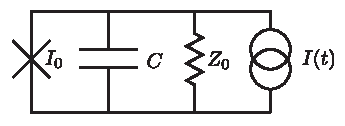
\includegraphics[width = 2.3in]{paramps_chapter/JPA_circuit}
\end{center}
\caption[Circuit model for LJPA]{Circuit model for a Josephson nonlinear resonator operated as a LJPA.  The nonlinear resonator is formed from the junction and capacitor at left, loaded by a transmission line modeled as a lumped impedance $Z_0$ and driven by an ideal current source $I(t)$.}
\label{fig:JPA_circuit}
\end{figure*}

The precise physics behind the operation of the LJPA is beyond the scope of relevance for this thesis, and has already been treated extensively in other works.  The general method to solve for the behavior of the LJPA is to start from the circuit model shown in Figure \ref{fig:JPA_circuit}.  Applying Kirchoff's laws permits the derivation of a differential equation for the junction phase difference $\delta(t)$, which will involve a nonlinear term proportional to $\sin[{\delta}(t)]$ due to the Josephson current-phase relation (\ref{eq:CPR}).  Approximating this term to the lowest nonlinear order of $\delta(t)^3$ results in the equation of motion of a classical Duffing oscillator, which can be explicitly solved for $\delta(t)$ in the presence of a strong drive.  This approach is described in detail in references \cite{slichterthesis,castaellanosthesis}.  Another approach, interesting for explicitly treating the quantum noise performance of the device, begins from the Hamiltonian for a first-order nonlinear harmonic oscillator, and is extensively described in reference \cite{eichlerthesis}.

\subsection{Performance and limitations of LJPAs}\label{s:jpa_perf}

We can consider a LJPA as a black box amplifier and characterize it using the figures of merit described in section \ref{s:amp_figures_of_merit}.  JPAs are generally operated with a gain of about 20 dB, sufficiently high to ensure that amplified input quantum fluctuations are much larger than the noise added by the following HEMT amplifier.  The input-referred noise temperatures can be close to the quantum limit, often within a factor of 2.  The main limitations for LJPAs are bandwidth and input power saturation, both of which are fundamentally related to the use of a nonlinear resonator as the geometry of the amplifier.

The need for a resonant geometry is essentially to enhance the coupling between the signal wave and the modulation of the Josephson junction.  The small-signal resonant frequency of this circuit is given by
\begin{equation}
\omega_0 = \frac{1}{\sqrt{L_JC}} = \sqrt{\frac{2\pi I_0}{\Phi_0 C}}.
\label{eq:w0_RLC}
\end{equation}
The bandwidth $B$ in the small-signal regime is related to the inverse of the quality factor, given simply by the standard equation for a LC oscillator damped by the coupling to a feedline of real impedance $Z_0$
\begin{equation}
Q = \omega_0 Z_0 C
\label{eq:Q_RLC}
\end{equation}
where $B \sim \omega_0/Q$.  This is a good approximation for large values of $Q$, but not entirely correct for small $Q$.  As the resonator is driven near resonance by a strong pump, the parametric process leads to gain as well as a reduction in bandwidth.  This tradeoff is known as the \textit{gain-bandwidth product}, and is roughly expressed as
\begin{equation}
B\sqrt{G} \propto \frac{1}{Q}.
\label{eq:g_bw_prod}
\end{equation}

Typical gain-bandwidth products for LJPAs are on the order of 100 MHz, implying $B = 10$ MHz with 20 dB gain \cite{Castellanos-Beltran2007,JPCNature,Hatridge:2011zr}.  Some devices have been demonstrated with gain-bandwidth products on the order of 1 GHz 
\cite{Mutus2014}.

The input compression power is determined by the amount of pump power available for amplification.  Roughly speaking, for the amplifier to remain linear, the fraction of the energy in the pump transferred to the signal should be very small, on the order of 1\% or -20 dB.  For an amplifier with 20 dB gain, this implies that the 1 dB compression power will be about 40 dB smaller than the pump power.  The maximum pump power than can be utilized is limited by the nonlinear dynamics of the resonator and is typically constrained to be 5-10\% of the critical current \cite{slichterthesis}.  For typical parameters, the 1 dB compression power is about -130 dBm \cite{Hatridge:2011zr}, though improved devices have enhanced this by as much as 20 dB \cite{Eichler2014a,Mutus2014}.

The gain-bandwidth product is the most challenging design constraint in improving the performance of LJPAs.  To increase both the gain of the amplifier and the bandwidth simultaneously, we can decrease $Q$.  We cannot make $Q$ arbitrarily small, however, as eventually higher-order nonlinear processes become important and prevent stable amplifier operation.  An approximate requirement for stability is
\begin{equation}
Q p \gtrsim 5
\label{eq:Q_p_prod}
\end{equation}
where $p = L_J / L_{tot}$ is the participation ratio of the Josephson inductance to the total inductance \cite{Weber2014a}.  In general there will always be some stray inductance which constrains $p < 1$.

We typically wish to keep the center frequency $\omega_0$ of the amplifier fixed at some specific value, requiring that we maintain a fixed ratio $I_0 / C$.  Thus, if we decrease $Q$ by making $C$ smaller, we must also reduce the junction critical current, thus reducing the input compression power.  One possible way to avoid this problem is by decreasing the environmental loading impedance $Z_0$ instead of $C$ by utilizing an impedance transformer to convert the standard 50 $\Omega$ environment to a lower value.  One device has been demonstrated with $Z_0 = 15$ $\Omega$ and realized a remarkably large bandwidth, though much of this improvement was related to a coincidental frequency dependence in $Z_0$ formed by the long propagation length of the impedance transformer rather than the reduction in $Z_0$ itself \cite{Mutus2014}.

One final constraint intrinsic to LJPA operation is the necessity of a separate non-reciprocal circuit element.  A resonator-based amplifier is intrinsically a 1-port device; this can be intuitively understood by the simultaneous need to efficiently couple the input signal to the resonator and efficiently couple the amplified field back out.  For a simple geometry, due to the reciprocal nature of the circuit topology, any port into the device that functions as an input will function just as effectively as an output.  Thus, the amplified output field leaves the amplifier through the same port through which it entered.  We must then use a non-reciprocal element to separate the outgoing signal mode from the incoming mode.  Microwave circulators are usually employed for this purpose, and do the job quite effectively.  However, these components are large, magnetic, expensive, and lossy.  Josephson-based parametric amplifiers with intrinsic directionality have been realized using a much more exotic circuit topology \cite{Abdo2014}, though the bandwidth and dynamic range of these devices are quite limited.

\section{Traveling-wave amplifiers}

For several applications of interest, the design constraints inherent in the LJPA are simply too stringent to realize an amplifier that simultaneously achieves large gain, large bandwidth, and large dynamic range.  For example, one common approach utilizing one amplifier and one transmission line to readout several qubits simultaneously is frequency-division multiplexing, which requires a bandwidth on the order of 50 MHz per qubit and power handling corresponding to about -110 dBm per qubit \cite{Barends2014,Riste2014}.  Furthermore, there are applications such as fault-tolerant quantum computing where the need for a circulator is a major impediment to scaling up the measurement system to thousands of qubits.  These constraints are inherent to the resonant geometry of the amplifier, so a natural question arises: is it possible to realize a Josephson amplifier that does not intrinsically utilize a resonant mode?

The inspiration for such a device comes from the optical domain.  Optical fibers have a weak, intrinsic nonlinearity which is exploited to make amplifiers \cite{Hansryd:2015uq}.  The general idea, then, is to exchange the enhanced coupling between the incident modes and the nonlinear element provided by the resonator for a very long co-propagation length through an extended nonlinear medium.  Because the pump and signal waves are now propagating in a single spatial direction, the gain provided by the amplifier is intrinsically directional and thus naturally operates as a 2-port device, eliminating the need for a external non-reciprocal element to separate the input and output modes.  The propagation length required in these optical fiber parametric amplifiers (OFPAs) is on the order of 100 m or more, owing to the very weak nonlinearities intrinsic to nonlinear optical systems.

In addition to the energy conservation criteria described previously (\ref{eq:4wave}), the traveling waves now also carry nonzero momentum, ascribed to the dispersion relation intrinsic to the waveguide in which the waves propagate.  For efficient mixing to occur, the process must conserve momentum; for four-wave mixing, we require
\begin{equation}
2 k_p = k_s + k_i
\label{eq:4wave_phase}
\end{equation}
where $k_x$ is the wavevector for mode $x \in \{p,s,i\}$.  This condition combined with (\ref{eq:4wave}) amounts to a constraint on the shape of the dispersion relation $k(\omega)$.  Since the spatial phase evolution of the modes is proportional to $k$, this momentum-matching constraint is generally called \textit{phase matching} in the literature of nonlinear optics.  Achieving phase matching is a central problem in nonlinear optical systems, and is likewise crucial to the efficient functioning of traveling-wave amplifiers.  I will leave a detailed discussion of this problem and its solution for chapter \ref{c:twpa_theory}.

\subsection{Josephson traveling-wave amplifiers}

Creating a superconducting amplifier analogous to a OFPA is not a new idea; a theoretical proposal for this type of device was made in 1985 \cite{Sweeny1985}, and an experimental realization of the device was created at Bell Labs in 1996 by Yurke \textit{et al} \cite{Yurke:1996ys}.  These works entirely ignored the issue of phase matching; furthermore, the Yurke device was created by loading the center trace of a co-planar waveguide (CPW) structure with 1000 Josephson junctions, producing a nonlinear transmission line with an impedance of 430 $\Omega$.  Because of this poor matching to the environment, the device was operated with one end shorted as a reflection amplifier and did not produce a compelling demonstration of traveling-wave performance.  The bandwidth of the amplifier was also quite small, only 125 MHz at a gain of 12 dB, comparable to a standard LJPA.

\begin{figure*}
\begin{center}
	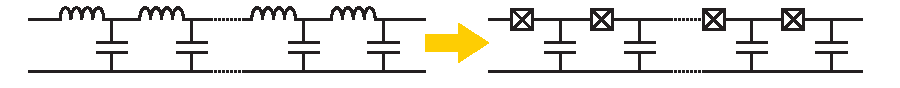
\includegraphics[width = 6in]{paramps_chapter/TWPA_circuit}
\end{center}
\caption[Circuit model for simple Josephson traveling-wave amplifier]{``LC ladder" lumped-element transmission line, and equivalent nonlinear lumped-element transmission line utilizing the Josephson inductance.}
\label{fig:TWPA_circuit}
\end{figure*}

\begin{figure*}
\begin{center}
	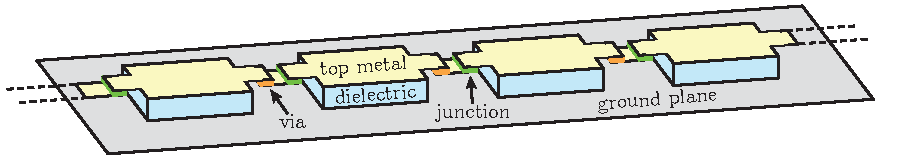
\includegraphics[width = 6in]{paramps_chapter/TWPA_geometry}
\end{center}
\caption[JTWPA in quasi-microstrip geometry]{A quasi-microstrip geometry to realize a low-impedance JTWPA.  The overall geometry looks something like a microstrip, with a center conductor (light yellow) situated on top of a ground plane (gray) with an intermediate dielectric layer (light blue).  Here, the center conductor is periodically interrupted by a Josephson junction (green).  A inter-layer via (orange) is used to make electrical contact with the bottom of the junction trilayer.}
\label{fig:TWPA_geometry}
\end{figure*}

Early attempts to produce a Josephson traveling-wave parametric amplifier (JTWPA) at QNL were performed by Ofer Naaman and Dan Slichter following the existing literature on the subject.  At this point in time the phase matching issue was not well understood, so early device designs looked much like straightforward nonlinear lumped-element transmission lines with Josephson junctions providing the inductance, as shown in Figure \ref{fig:TWPA_circuit}.  The main innovation at this point in time was the introduction of a new physical geometry for the transmission line; rather than utilizing a CPW structure as in the Bell Labs device, we created a kind of quasi-microstrip geometry shown in Figure \ref{fig:TWPA_geometry}.  By employing a parallel-plate capacitor geometry, the capacitance to ground per junction can be made much larger than in a CPW, allowing for the transmission line to be well matched to 50 $\Omega$.

Due to fabrication difficulties, these early devices never delivered breathtaking amplifier performance and were plagued by large, unknown losses; parametric gain was observed, however, encouraging continued development.  These results are described in Slichter's thesis \cite{slichterthesis}.  To understand what might be limiting this performance, we embarked on a major theoretical effort to understand the JTWPA, finally culminating in the practical device described in this thesis.  The full theory of the JTWPA and extensive experimental results are the subject of chapters \ref{c:twpa_theory} and \ref{c:twpa_exp}, respectively.























\chapter{Stabilization of Rabi oscillations: experimental setup}
\label{c:qfb}

With superconducting qubits, circuit QED, and nearly-quantum-limited parametric amplifiers in hand, we have all the tools needed to implement a quantum control protocol: namely, the stabilization of coherent Rabi oscillations of a qubit.  In this chapter I will describe the important aspects of the apparatus specific to the quantum feedback experiment; for excellent descriptions of the many important details in a general cQED apparatus, I refer the reader to Slichter's thesis \cite{slichterthesis} and Weber's thesis \cite{Weber2014a}.  The apparatus used for this experiment is a direct descendent from the setup described in Slichter's thesis, with relatively minimal modifications.  The weak dispersive regime of cQED---the relevant regime for this quantum feedback experiment---is also the basis for the experiments described in Weber's thesis.

\section{Relevant circuit QED parameter regime}

The scheme for demonstrating feedback control is explicitly an analog, continuous-time technique, which intrinsically creates an important hierarchy of rates in the cQED system and measurement apparatus.  We desire to create pure, sinusoidal Rabi oscillations of the qubit state, which implies that the Rabi rotation frequency $\Omega_r$ should be the fastest continuous rate in the system.  The time scale over which a measurement projects the qubit state should be much longer than one period of these oscillations, implying $\Gamma_m \ll \Omega_r$.  To ensure reliable operation of the feedback technique, we require that the rates corresponding to spontaneous relaxation and dephasing of the qubit are small compared to the measurement rate, $(\Gamma_1, \Gamma_\mathrm{env}) \ll \Gamma_m$.

Furthermore, since the feedback technique stabilizes the phase of qubit oscillations in a single plane through the Bloch sphere, we require that the back-action of the measurement correspond only to disturbances in the phase of this oscillation, not in any rotations of the qubit state in the equatorial plane.  As discussed previously in section \ref{s:cQED_backaction}, this implies that we should work in the limit of small phase shift, $2 \chi \ll \kappa$, and selectively measure only the signal quadrature containing qubit state information.  Satisfying $2 \chi \ll \kappa$ is straightforward by making the qubit-cavity coupling rate $g$ relatively small and the qubit-cavity detuning $\Delta$ relatively large.  To selectively measure the signal quadrature containing qubit state information, we use a LJPA operating in a phase-sensitive mode and align the amplification axis to this quadrature.  The result is that the photon number fluctuations in the cavity are squeezed, implying no measurement-induced pure dephasing of the qubit state due to the lack of photon number fluctuations.  This ensures that the measurement back-action does not cause the qubit state to diverge from the relevant plane of the Bloch sphere, allowing for an efficient single-parameter feedback.

\section{Experimental setup}

\begin{figure*}
\begin{center}
	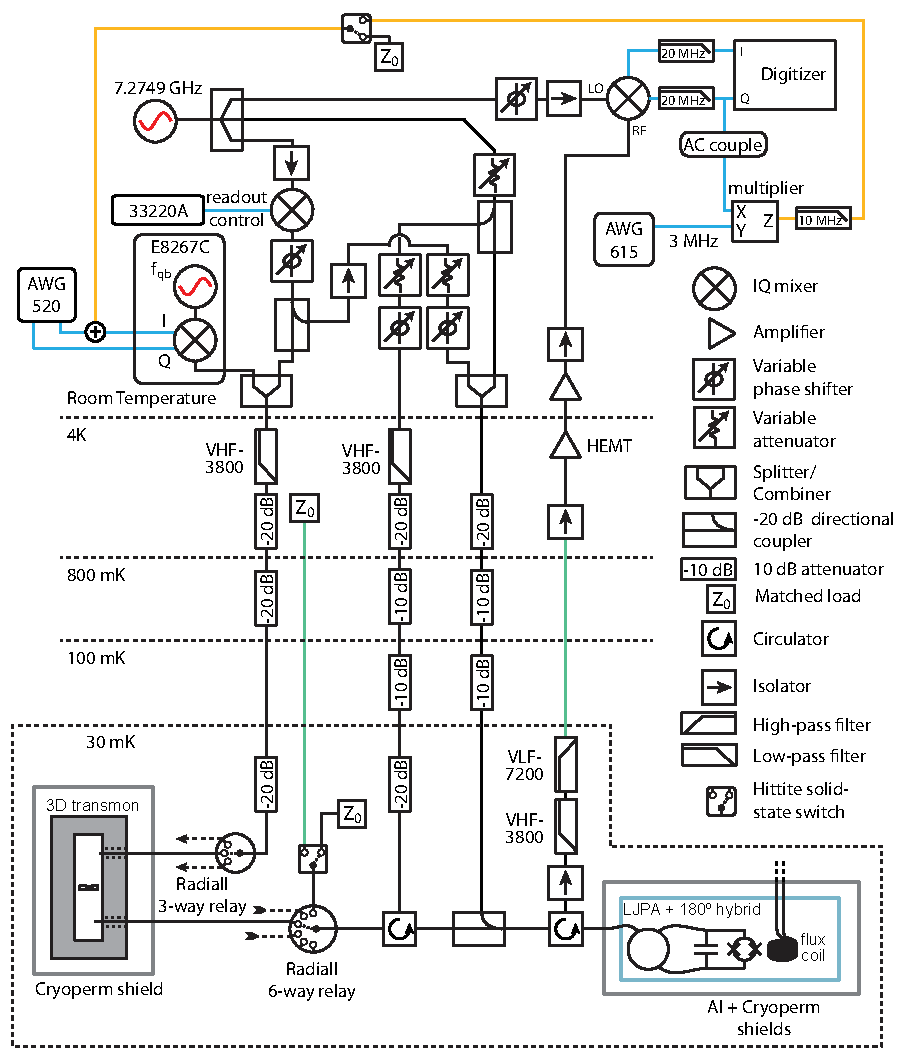
\includegraphics[width = 6in]{qfb_exp_chapter/full_schematic}
\end{center}
\caption[Experimental setup for quantum feedback]{Experimental setup for quantum feedback experiment.  Microwave signals paths are drawn as black lines, low-frequency signal paths are light blue, and the feedback error signal is drawn as an orange line.  The exception to this rule are the segments of low-loss superconducting coax lines linking 4K and 30 mK, drawn as green lines.}
\label{fig:full_schem}
\end{figure*}

A fairly complete schematic of the experimental setup for the feedback experiment is shown in Figure \ref{fig:full_schem}.  The primary missing element not shown is the trigger cascade used to control the timing in the experiments; however, the exact trigger configuration is not entirely constant across different experiments and is not as important as the signal routing.  Also omitted are low-frequency cryogenic control lines, as they are mostly used for DC biasing and are not changed during a particular experimental run.

\subsection{Qubit and parametric amplifier}

At the bottom of Figure \ref{fig:full_schem}, the primary elements of interest are the 3D transmon qubit system, at left, and the LPJA (paramp), at right.  The 3D transmon consists of a single-junction transmon qubit with transition frequencies $\omega _{01}/2\pi =5.4853$ GHz and $\omega _{02}/2\pi =10.7382$ GHz. From these values, we calculate $E_J=19.274$ GHz and $E_C=0.211$ GHz giving $E_J/E_C = 91$.  The transmon is fabricated on a bare high-resistivity Si wafer using electron beam lithography and double-angle aluminum evaporation with an intervening oxidation step.  For additional details on qubit fabrication, see references \cite{slichterthesis,Weber2014a}.  The transmon is antenna-coupled to an aluminum waveguide cavity with resonant frequency $\omega _{c}/2\pi =7.2756$ GHz when the qubit is in the ground state. The strongly coupled output port sets the cavity linewidth $\kappa/2\pi=13.4$ MHz while control and measurement signals are injected via the weakly coupled input port.  We use relay switches to multiplex several different 3D transmon systems in a single cooldown, though we only used one device in the feedback experiment so the others are not drawn.\footnote{In some calibration experiments in this dilution refrigerator, the presence of the relay switches seemed to reduce qubit $T_2$ times, though this was likely due to a lack of filtration on the switch wiring as well as the fact that the backs of the switch bodies were open and thus a potential source of stray infrared light.} The 3D transmon resides in a single-layer cryoperm magnetic shield.  Qubit control pulses are straightforward square-envelope pulses sourced from a Tektronix AWG 520 driving the IQ inputs of a Agilent E8267C vector signal generator.

The paramp is differentially excited using a 180$^\circ$ rat-race hybrid; the amplifier center frequency is tuned by a variable flux induced by a nearby superconducting coil.  The paramp is pumped using a single tone degenerate with the cavity frequency, enabling phase-sensitive detection of the qubit measurement signal.  This tone is sourced from a single microwave generator and split several ways, ensuring a stable phase relationship between the measurement tones.  Because there are five different arms in what amount to a interferometric arrangement, at least 4 phases must be independently tuned.  This is accomplished with analog phase shifters on each signal arm besides the pump for the paramp; because the first step in the experiment is tuning the paramp bias conditions, we want these conditions to remain fixed, and the phase shifters do not have flat insertion loss as the phase is adjusted.  The paramp is biased up for 24 dB gain with a large bandwidth of about 80 MHz FWHM, due to a fortuitous ripple in the environmental impedance.  A room-temperature variable attenuator sets the pump amplitude.

The qubit measurement signal is shaped by a low-frequency Agilent 33220A arbitrary waveform generator driving one port of a mixer.  This signal is injected into the fridge on the same signal line as qubit control pulses.  This line is heavily attenuated and then connected to the weakly coupled port of the 3D cavity.  The coupling of this port is designed to be approximately -20 dB, ensuring that virtually all of the measurement signal leaves the cavity through the strongly coupled port.  The measurement signal is routed to the LJPA where it undergoes phase-sensitive amplification.  This signal is then routed back to room temperature via the HEMT amplifier and into one or two stages of room temperature amplification.  This signal is then demodulated in a homodyne measurement setup using an IQ mixer, and the I and Q quadratures are filtered and digitized at 100 MS/s.  The relative phase of the measurement signal and paramp pump are aligned so that the amplification axis corresponds to the IQ axis containing qubit state information.  The phase of the homodyne local oscillator is adjusted to place the amplified axis entirely in the Q quadrature of the digitizer.  This eliminates any need to calibrate the two quadratures of the homodyne setup, which in general have different gain and represent axes which are not perfectly orthogonal to each other.  This is done in practice by adjusting the local oscillator phase and measuring the noise power detected in each output quadrature.  Minimizing the noise power in the I quadrature corresponds to aligning the amplification axis with Q.


\subsection{Feedback circuit}

The feedback portion of the circuit is quite straightforward.  Because the demodulated output signal from the experiment can be directly interpreted as a noisy estimate of $\xpec{\sigma_z}$, no complex digital signal processing is required to give physical significance to the output signal.  This is in contrast to more complex feedback schemes that rely on reconstructing the density matrix in real time and conditioning a feedback signal based on the error between the reconstructed density matrix and the target state \cite{PhysRevA.69.052324,Zhang2005}, which requires complex digital electronics (typically implemented in an FPGA).

The key component needed to implement the direct feedback protocol is an analog multiplier.  At low frequencies, inexpensive integrated circuits that perform a true analog multiplication are available.  In this experiment, the analog multiplier is made by Analog Devices, part number AD835a.  This chip has a large -3 dB bandwidth of 250 MHz, ensuring very linear operation at our feedback frequency of 3 MHz.  The multiplier is housed on a small custom PCB.  Over the course of the experiment we explored several arrangements of filters at the input and output of the feedback controller, including various single-pole and multi-pole filters implemented in a commercial tunable filter (Krohn-Hite 3945).  We eventually removed all of this filtering, as the intrinsic bandwidth of the LJPA combined with the filters at the output of the demodulation stage provided more than enough rejection of uncorrelated noise.  We did keep the Krohn-Hite in the input to the feedback circuit, but exclusively used as high-pass filter with a very low frequency cutoff to effectively AC-couple the multiplier input circuit.  This is critical, as the demodulation setup includes a large DC offset which can drift over time.  Although the feedback routine is continuous, any given experiment takes place over a relatively finite and short time scale so true DC response is not necessary.  Adding this AC coupling stage ensures that the signal corresponding to the qubit oscillations and amplified quantum noise remains centered about $V = 0$.

The reference signal for the feedback loop was originally sourced by a low-frequency RF signal generator.  This was adequate for assessing the performance of feedback in the frequency domain, but insufficient for time-domain analysis as the phase of the reference signal at the start of the experiment was uncorrelated between iterations.  Instead, we create a synthesized 3 MHz reference signal using a Tektronix AWG 615 triggered as part of the trigger cascade.  This ensures a stable reference phase for the feedback reference signal.  The total feedback gain $F$ is adjusted by controlling the amplitude scale on the output of this AWG.

\section{Calibration experiments}

Interpreting the results of the feedback control loop in the context of the theoretical description demands a precise calibration of both the typical cQED and amplifier parameters.  Additionally, there are several parameters of direct interest to the feedback control theory which must be separately measured or inferred.

\subsection{Dispersive shift and cavity photon number occupation}\label{s:chi_cal}

\begin{figure*}
\begin{center}
	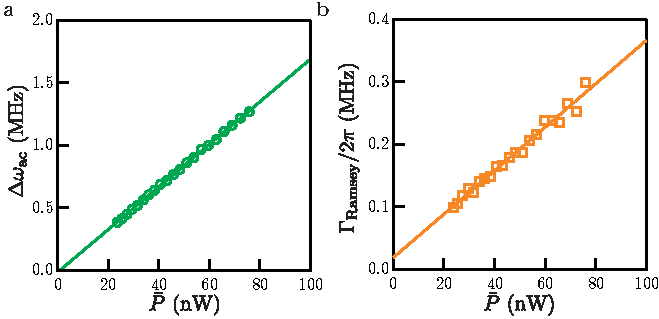
\includegraphics[width = 4.39in]{qfb_exp_chapter/chi_cal}
\end{center}
\caption[AC Stark shift and dephasing rate]{Measurements of AC Stark shift and measurement-induced dephasing rate vs. weak measurement power with linear fits.  \textbf{a} Qubit frequency shift as a function of measurement power.  Multiplying these values by the calibrated value for $2\chi$ results in the extracted value for $\bar{n}$ as a function of input power.  \textbf{b} Ramsey dephasing rate as a function of measurement power.  The offset at zero measurement power corresponds to the total environmental dephasing rate (including non-idealities such as $T_1$).}
\label{fig:chi_cal}
\end{figure*}

Many qubit and cavity parameters can be directly measured through spectroscopic means.  The cavity frequency and linewidth are measured by fitting the transmission spectrum to a Lorentzian function.  The qubit transition frequencies are measured spectroscopically.  The coherence times of the qubit are also easily measured using standard pulse sequences.  We measure $T_1 = 20$ $\mu$s using a $\pi$-pulse with a variable delay, and $T_2 = 8$ $\mu$s using a standard one-pulse spin echo sequence.

In order to determine the dispersive shift $\chi$, we use a combination of the AC Stark shift
\begin{equation}
\Delta \omega_{ac} = 2\chi \bar{n}
\label{eq:ac_stark}
\end{equation}
and measurement induced dephasing of the qubit
\begin{equation}
\Gamma_{\varphi} = 8\chi^2 \bar{n}/\kappa,
\label{eq:gamma_phi}
\end{equation}
where $\bar{n}$ is the average photon occupation of the readout cavity \cite{schusteracstark}. To measure these quantities precisely, we perform a Ramsey fringe experiment where the free evolution period between the two $\pi / 2$ pulses is modified by exciting the cavity with a fixed power $\bar{P}$ at the readout frequency $\omega_{\rm r}$. By fitting the Ramsey fringes to an exponentially decaying sinusoidal function, we measure $\Delta \omega_{ac}$ by extracting the Ramsey frequency and $\Gamma_{\varphi} = \Gamma_{\rm Ramsey} - \Gamma_2^*$ by extracting the decay constant. Here $T^\ast_{2} = 1/\Gamma^\ast_{2}$ is the decay constant of the Ramsey fringes in the absence of any photons in the cavity. This technique is significantly faster than conventional spectroscopy \cite{schusteracstark} and provides better precision in extracting $\Delta \omega_{ac}$  and $\Gamma_{\varphi}$. We repeat this process for different $\bar{P}$; since $\bar{n} \propto \bar{P}$, a plot of $\Delta \omega_{ac}$ vs $\bar{P}$ and $\Gamma_{\mathrm{Ramsey}}$ vs $\bar{P}$ gives two straight lines with slopes $m_{ac}$ and $m_{\varphi}$ (Figure. \ref{fig:chi_cal}). The ratio $m_{\varphi}/m_{ac} = 4\chi/\kappa$ then allows us to determine the dispersive shift $2\chi / 2 \pi = 1.375$ MHz. We use this value of $2\chi$ and the Stark shift data to calibrate the mean photon number $\bar{n}$ in the cavity.

\subsection{Paramp pump cancellation}

Because the strong pump for the paramp is degenerate with the measurement frequency, the cavity must be well-isolated from this signal.  Stray photons from the paramp pump which leak backwards into the cavity result in measurement-induced dephasing even in the absence of a measurement signal.  Adding additional isolation elements between the cavity and paramp will improve the isolation by approximately 20 dB per isolator, at the expense of about 1 dB of signal insertion loss in each isolator.  Because we aim to realize a highly efficient measurement apparatus, we must take great pains to minimize the signal loss between the cavity and paramp.

Due to the reflection geometry of the paramp, we require at least one circulator to separate input and output modes.  Furthermore, from the discussion in section \ref{s:jpa_perf}, the pump power must be about 40 dB larger than the input signal, implying that 40 dB of isolation (two isolator elements) would still result in a large stray signal in the cavity, on the order of our largest measurement signal.  We aim to make the dephasing due to the stray pump leakage much smaller than the intrinsic environmental dephasing rate $\Gamma_\mathrm{env}$.  From \eqref{eq:gamma_phi}, for $\Gamma_\mathrm{leakage} < 0.1 \Gamma_\mathrm{env}$, that places an upper limit on the photon number in the cavity $\bar{n}_\mathrm{leakage} < 0.007$, or a power incident on the cavity of less than $P_\mathrm{leakage} < -175$ dBm.  Typical pump powers are on the order of -90 dBm, implying a need for about 80 dB of isolation.  The $\sim$4 dB loss from using four circulators would imply a maximum measurement efficiency $\eta = 0.4$, much smaller than unity.

To avoid this issue, we use two circulators rather than four, providing $\sim$40 dB of isolation.  To achieve the additional isolation needed, we connect another signal line to the third port of the first circulator as shown in Figure \ref{fig:full_schem}.  At room temperature, we tap off a small portion of the paramp pump using a directional coupler, and pass this signal through a variable attenuator and a phase shifter and inject it into this extra signal line.  The circulator directs this signal back towards the strongly coupled port of the cavity and is thus co-propagating with any pump leakage.  By carefully tuning the attenuation and phase shift with the paramp pump energized, this extra \textit{pump cancellation signal} interferes destructively with the leakage signal.

The pump cancellation attenuation and phase is tuned by hand while Ramsey oscillations of the qubit are continuously measured, using the AC Stark shift of the qubit as a very sensitive power meter.  When the AC Stark shift is nearly zero compared to the value measured with the pump off, the pump signal has been well cancelled.  This is also reflected in the dephasing rate extracted from the same experiment.  Due to the linearity of the microwave injection lines and the fact that the pump cancellation signal is split from the pump after the attenuator which controls the pump amplitude, once the attenuation and phase are set for the pump cancellation signal, the cancellation remains perfect even when the pump amplitude is adjusted.  Changing the pump frequency requires re-tuning the cancellation signal.

Shortly after this experiment concluded, an alternative pumping technique known now as ``double-pumping'' came into favor, where the paramp is driven by two strong pump tones symmetrically detuned above and below the center frequency \cite{PhysRevB.79.184301}.  This technique significantly eases the issue of pump cancellation, as the drive tones can be detuned by several hundred megahertz, ensuring that the total power leaking back towards the cavity is well-filtered by the cavity response function.  For details on the experimental implementation of this technique, see reference \cite{Weber2014a}.


\subsection{Dumb signal cancellation}

\begin{figure*}
\begin{center}
	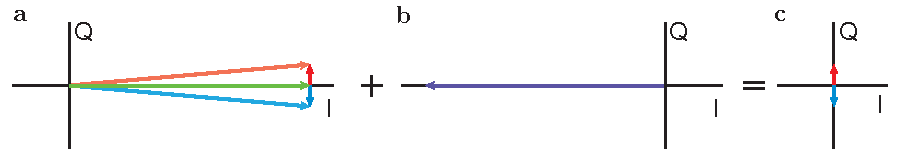
\includegraphics[width = 6in]{qfb_exp_chapter/dumb_sig}
\end{center}
\caption[Dumb signal cancellation]{\textbf{a} IQ vector diagram showing the coherent state vectors for the ground state (pale blue) and excited state (pale red), and the decomposition of those vectors into the qubit state components (dark red and dark blue) and the component which contains no qubit state information (green), the dumb signal.  \textbf{b} A coherent tone phase-shifted by 180 degrees with identical amplitude to the dumb signal.  \textbf{c} The coherent addition of these vectors results in only the pure qubit state component without the large extra signal power associated with the dumb signal.}
\label{fig:dumb_sig}
\end{figure*}

Because this experiment is conducted in the limit where $\chi \ll \kappa$, the phase shift between the output signals is quite small.  Thus, to achieve large signal-to-noise ratio in a projective measurement of the qubit, the cavity occupation $\bar{n}$ must be increased to separate the qubit state histograms.  In the IQ plane, we can decompose this signal into two components: the component in the quadrature which contains qubit state information, and the component in the other quadrature which will be squeezed by the parametric amplifier.  This vector decomposition is shown in Figure \ref{fig:dumb_sig}.  The vast majority of the power in the signal is in the quadrature which contains no information about the qubit state; we call this the \textit{dumb signal} as it ``knows nothing'' about the qubit state.  Ideally, the paramp will squeeze this quadrature away.  However, the alignment between the paramp and signal phase is never perfect, and this extra power can cause input compression if the phase angle is slightly misaligned and part of this power ends up in the amplified quadrature.

\begin{figure*}
\begin{center}
	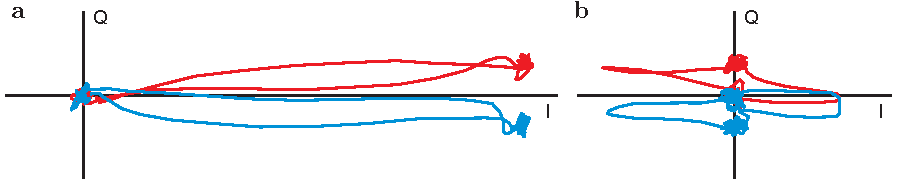
\includegraphics[width = 6in]{qfb_exp_chapter/dumb_sig_exp}
\end{center}
\caption[Dumb signal cancellation data]{\textbf{a} Measured IQ trajectories for the ground state (blue) and excited state (red), showing the large dumb signal component.  Axes have a square aspect ratio with arbitrary units.  Trajectories start and end at the origin, so the loops correspond to the ring-up and ring-down of the resonator.  \textbf{b} The same trajectories with the addition of the optimized dumb signal cancellation path.  The separation at steady-state is the same, but the large extra signal power has been cancelled.  Axes have the same scaling as in \textbf{a}.}
\label{fig:dumb_sig_exp}
\end{figure*}

We avoid this problem by tapping off a portion of the qubit measurement signal at room temperature using a directional coupler, passing this signal through a variable attenuation and phase shifter, and adding it to the paramp pump signal.  With the paramp pump off, the amplitude and phase shift of this \textit{dumb signal cancellation signal} is adjusted by hand to draw the IQ histograms for the qubit ground and excited states back towards the origin.  This optimization is relatively easy compared to the paramp pump cancellation tuning procedure, as the cancellation does not need to be particularly precise.  Actual measured IQ trajectories for the ground and excited states are shown in Figure \ref{fig:dumb_sig_exp}a.  This type of plot is used to adjust the amplitude and phase of the dumb signal cancellation signal until the steady-state trajectories are centered at the origin, as shown in Figure \ref{fig:dumb_sig_exp}b.  With the dumb signal component well cancelled, small phase mismatches between the signal and paramp pump no longer result in paramp compression during projective readout.  Just like for pump cancellation, because of the circuit topology and the linearity of the intermediate circuit components, once the amplitude and phase are adjusted, the cancellation works well for any pulse amplitude or duration.  There are still some transient effects during ring-up and ring-down due to the finite resonator bandwidth, but these are not important for good steady-state readout performance.

\subsection{Detector and measurement efficiency}\label{s:det_meas_eta}


The overall measurement efficiency relevant for feedback is given by $\eta = \eta_{\mathrm{det}} \ \eta_{\mathrm{env}}$. The first term $\eta_{\mathrm{det}}$ accounts for the noise added by the amplification chain. To measure this noise, we use the qubit-cavity system as a calibrated signal power source. As discussed in section \ref{s:chi_cal}, we can excite the cavity with a precise average photon occupation $\bar{n}$. This corresponds to an RMS power radiated from the cavity $P_{\mathrm{rad}}= \hbar\omega_{r} \kappa \bar{n}$, where $\omega_{r}$ is the frequency of excitation. We send this signal to the paramp and measure the signal-to-noise ratio (SNR) at the output. This allows us to extract the noise floor of the entire measurement chain referred to the output plane of cavity, which includes dominant contributions from the signal loss between the cavity and paramp and imperfections in the paramp itself, as well as a smaller contribution from the noise added by the HEMT amplifier. 

The noise floor referred to the input of the amplification chain is given by $P_{\rm n} = \hbar \omega_{r}B/\eta_{\rm det}$, where $B$ is the integration bandwidth (in Hz).  The signal-to-noise ratio can then be expressed as
\begin{equation}
\mathrm{SNR}=\frac{P_\mathrm{rad}}{P_\mathrm{n}}.
\end{equation}
Substituting in the expressions for $P_\mathrm{rad}$ and $P_\mathrm{n}$, we can solve for the detector efficiency in terms of the measured SNR, yielding the expression
\begin{equation}
\eta_{\rm det}=\frac{{\rm (SNR)}}{   \bar{n}} \frac{B }{ \kappa}.
\end{equation}
This definition of $\eta_{\rm det}$ is consistent with phase-sensitive operation of the paramp and measures the departure from the best SNR we could possibly obtain when amplifying at the quantum limit. We measure the SNR for a range of frequencies within the paramp bandwidth and extract an average detector efficiency $\eta_{\rm det}=0.46$.  Using cryogenic switches, separately measure the attenuation between the cavity and the paramp to be roughly 2.5 dB, implying that signal attenuation is the dominant source of reduction in detector efficiency.

 The final contribution to the overall measurement efficiency is due to environmental decoherence via pure dephasing. The efficiency $\eta_{\mathrm{env}} = (1+\Gamma_{\mathrm{env}} / \Gamma_{\varphi})^{-1}$ characterizes how much of the total dephasing is due to measurement. In principle we could improve this efficiency by increasing $\bar{n}$ (and thus $\Gamma_{\varphi}$), but there are two practical constraints. First, the measurement must be weak enough that it is not projective on the timescale of the Rabi period $\Omega_{\rm R}^{-1}$, ensuring the qubit evolution remains mostly oscillatory. Second, the required feedback bandwidth increases with $\Gamma_{\varphi}$. Since the effective feedback bandwidth is fixed by the measurement chain, the feedback efficiency $D$ decreases with increasing measurement strength if $\Gamma_{\varphi}$ becomes too large.  Dephasing due to low frequency noise does not affect the feedback efficiency because the system can track any slow variations in the qubit frequency (and consequently in the Rabi frequency). Hence, we set $\Gamma_{\mathrm{env}} = 1/T_2$ measured from echo experiments giving us $\Gamma_{\mathrm{env}}/2\pi = 0.02$ MHz, and $\eta_{\mathrm{env}}=0.87$.  This definition includes the dephasing contribution from qubit relaxation ($\Gamma_1 / 2$).


\subsection{Projective measurement and qubit temperature}

Because we realize a high-quantum-efficiency measurement chain, making a faithful projective measurement is simply a matter of acquiring sufficient SNR to separate the histograms corresponding to the ground state and excited state in a time much shorter than the qubit relaxation time.  We use a photon number $\bar{n} = 11$ and an integration time of 800 ns to acquire well-separated histograms.  This integration time is not negligible compared to $T_1$, so the fidelity of the readout is primarily constrained by this.  For most experiments of interest, this reduction in fidelity from unity is not important so long as the fidelity remains high, on the order of 90\% or more, such that SNR remains high.  A discussion of how imperfect readout fidelity is calibrated out of the results appears in section \ref{s:qst_cal}.

\begin{figure*}
\begin{center}
	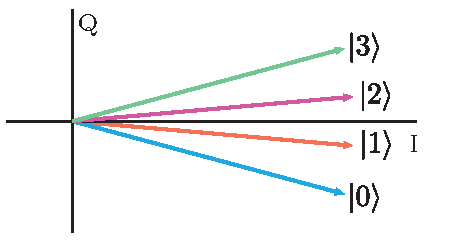
\includegraphics[width = 3in]{qfb_exp_chapter/qutemp_IQ}
\end{center}
\caption[IQ vectors for multi-state readout]{IQ vector diagram showing the coherent state vectors for the first four qubit states.  By aligning the phase of the measurement signal to be roughly centered on the phase between the states $\ket{1}$ and $\ket{2}$, the total phase shifts are small enough to be measured simultaneously without compressing the paramp.}
\label{fig:qutemp_IQ}
\end{figure*}

Since the cQED system is optimized to the weak measurement regime where the phase shift between qubit states is small, it is possible to measure more than just the $\{ \ket{0},\ket{1} \}$ manifold.  An IQ diagram showing the coherent state vectors corresponding to several qubit states in an idealized representation is shown in Figure \ref{fig:qutemp_IQ}.  Each qubit state above $\ket{1}$ shifts the resonant frequency of the cavity by (approximately) an additional amount $2 \chi$, such that the signal phase can be adjusted to observe the readout histograms for several states simultaneously.  The actual shift for the higher states is somewhat smaller than $2 \chi$, but this detail is not important here.

\begin{figure*}
\begin{center}
	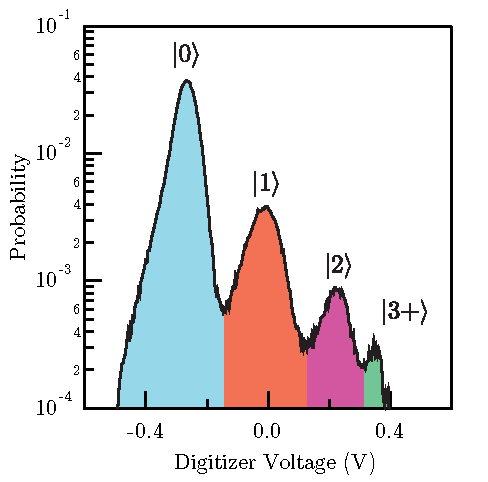
\includegraphics[width = 3.25in]{qfb_exp_chapter/qutemp}
\end{center}
\caption[Qubit temperature histograms]{Readout histograms showing non-trivial occupation of energy levels above the ground state.  The state occupations are $P_0 = 0.83$, $P_1 = 0.13$, $P_2 = 0.03$, and $P_{3+} = 0.01$.}
\label{fig:qutemp}
\end{figure*}

Due to the high single-shot fidelity of the readout, we can measure the temperature of the qubit in thermal equilibrium simply by measuring an ensemble of qubits with no explicit state preparation.  After each measurement, we wait for approximately $10 \ T_1$ to allow the qubit to re-thermalize.  Histograms of this measurement are shown in Figure \ref{fig:qutemp}.  The distribution of state occupation probabilities does not obey a Boltzmann distribution, so it is not precisely a thermal state.  However, if we approximate the system by only considering the first two levels, we can approximate the distribution as thermal and assign a temperature of approximately 140 mK, much higher than the thermal temperature of the dilution refrigerator (about 30 mK).  This type of spurious excited state population has been observed in other experiments \cite{fluxqb,Geerlings2013,Jin2014} and was common for superconducting qubits of this era.  It is now reasonably well understood that that these large spurious populations are due to quasiparticle excitations created by stray infrared photons.  Enhancing the degree to which the qubits are shielded from stray light has been shown to enhance coherence times and significantly reduce the spurious thermal population \cite{Barends2011}.

Because the readout is QND, we can use the readout itself to artificially create an ensemble of qubits which are perfectly prepared in the ground state through post-selection.  The protocol is to insert a projective measurement pulse at the start of the experiment, and then perform the experiment as usual.  When the data is analyzed, any experimental records in which the qubit did not start in the ground state are thrown out, creating a post-selected ensemble in the ground state at the cost of throwing away the fraction of the data corresponding to the spurious excited state population.  The first application of this post-selection cooling technique was the subject of a separate work published in Physical Review Letters \cite{fluxqb}.  The technique of purifying ensembles using post-selection and the QND nature of the cQED readout is quite useful for removing experimental imperfections in general, and is applied in numerous places in the work in this thesis.

\subsection{Quantum state tomography}\label{s:qst_cal}

Fully reconstructing the quantum state of a qubit requires measuring an ensemble of identically-prepared qubits along at least three different qubit measurement axes.  The cQED measurement naturally probes the qubit state in the $\sigma_z$ basis, so an ensemble of measurements provides $\xpec{\sigma_z}$.  To measure $\xpec{\sigma_x}$ ($\xpec{\sigma_y}$) we must first rotate the qubit state by an angle $\pi/2$ about the $\hat{y}$ ($-\hat{x}$) axis (respectively).  These expectation values define the Bloch vector components and thus the density matrix of the qubit state.

To ensure accurate tomographic results, the measurement and qubit manipulation pulses must be precisely calibrated.  After single-shot measurement is tuned up (mostly a matter of aligning the signal and paramp phase and tuning the measurement power and integration time), we can precisely calibrate a $\pi$-pulse by adjusting the pulse amplitude until we maximize $P(\ket{1})$.  Because of the finite measurement fidelity due to qubit relaxation during readout, $P(\ket{1})$ will never go all the way to 1; this implies that even if we prepare the excited state, we would not measure $\xpec{\sigma_z} = -1$.  This effect is easy to correct for by measuring the values of $P(\ket{1})$ for the ground state ($P_g$) and the excited state ($P_e$).  Then, when we measure $P(\ket{1})$ for an experimental ensemble, we re-scale it as 
\begin{equation}
P(\ket{1})' = \frac{P(\ket{1}) - P_g}{P_g + P_e}.
\end{equation}
Since $P(\ket{2+})$ is not negligible, we use post-selection to eliminate experimental records where the qubit was found outside the $\{ \ket{0},\ket{1} \}$ manifold.  Because none of the control pulses are resonant with any transition involving the higher qubit states, this post-selection essentially eliminates the effect of thermal excitation out of the $\{ \ket{0},\ket{1} \}$ manifold on the tomographic reconstruction of the target state, improving both the tomographic quality as well as the quality of the measured state itself.

We utilize a series of combination pulses to calibrate the $\pi/2$ pulses on $\hat{y}$ and $-\hat{x}$.  We calibrate the amplitude of the $\pi/2$ pulses by adjusting the pulse amplitudes until $P(\ket{1})' = 0.5$ for each.  We verify that the $\pi$ and $\pi/2$ pulses are balanced by measuring $P(\ket{1})'$ for a $\pi$ pulse immediately followed by a $\pi/2$ pulse, and ensuring that $P(\ket{1})'$ is still maximized for $\pi$ while $P(\ket{1})' = 0.5$ for the bare $\pi/2$ and the $\pi + \pi/2$ sequence.  We then check the orthogonality of the $\hat{y}$ and $-\hat{x}$ axes by measuring two sequences that have two $\pi/2$ pulses in sequence, one on each axis.  Deviations from $P(\ket{1})' = 0.5$ indicate that the two axes are not perfectly orthogonal.  We utilize the vector generator's built-in quadrature skew correction feature to null this effect to the couple-percent level.  This entire optimization sequence is somewhat challenging, as the quadrature skew correction also effects the balance of the I and Q inputs, requiring the absolute and relative amplitudes of the pulses to be re-adjusted.  All in all this procedure is iterated a few times until all of the pulses are in balance; at this point, the system is essentially stable aside from overall RF level fluctuations, which are easily controlled.  In reality, all of these pulses are programmed into a single AWG sequence along with a given experiment of interest, thus monitoring the quality of tomography during the experiment.

We make no attempt to include any error amplification or self-consistency techniques in the calibration sequence \cite{Chow2009,Merkel2013,Blume-Kohout2013}; as such, this calibration technique is somewhat ``rough and ready,'' but insufficient to achieve calibration better then the few percent level.  Because the measurement efficiency in this experiment is about 0.4 and the feedback efficiency $D$ and thus the stabilized Bloch vector amplitude is constrained to be less than $\sqrt{\eta} = 0.63$, a few percent error in the pulse calibrations is tolerable to reasonably well characterize $D$.  Contemporary experiments in the lab utilize more sophisticated calibration techniques, including error amplification by repeated pulses.  Furthermore, we now typically use single-sideband modulators instead of IQ mixers, sidestepping the issue of quadrature skew correction entirely and allowing full Bloch sphere control of one qubit from a single AWG channel by utilizing finite-frequency pulses.

\subsection{Loop delay}\label{s:loop_delay}

The quality of the feedback control will depend on the total round trip delay time $\tau_{\rm delay}$ between a measurement signal leaving the cavity and the corresponding feedback correction entering the cavity.  This delay can be broken into two pieces: the delay in the microwave-frequency part of the system and the delay in the low-frequency part of the system.  The microwave delay includes the propagation time through the transmission lines into and out of the experiment, and also implicitly includes the bandwidth of the microwave cavity and paramp.  Because the cavity has a relatively large bandwidth, $1/\kappa \sim 10$ ns, and only contributes to the measured value of $\tau_{\rm delay}$ at the few percent level.  We measure the microwave delay by injecting a $\pi$-pulse into the fridge while the qubit is being weakly measured.  We tap off a portion of the voltage envelope that drives the IQ mixer, and feed it to the I channel of the digitizer (properly accounting for extra cable length for signal routing).  We then measure the delay between the arrival of this pulse at the digitizer and the arrival of the leading edge of the shift in resonator phase on the Q channel, resulting in $\tau = 200$ ns ($\pm$ 10 or 20 ns or so).  Measuring the delay in the low-frequency portion of the measurement chain is a straightforward matter of measuring pulse propagation delay using an oscilloscope, a total delay of about 80 ns, for a grand-total loop delay of about 280 ns.

\subsection{Feedback strength calibration}

The theory for feedback stabilization is expressed using a dimensionless feedback strength parameter $F$ which takes into account all of the relevant gain stages in the system.  To compare to theory, we must calibrate the feedback loop to determine the gain in normalized units.  First, we use the digitizer to measure the full voltage swing $\Delta V$ in the output of the demodulation setup between the qubit being in the ground state vs. the excited state for a given measurement strength.  We use post-selection on an initial and final strong measurement pulse to prepare an ensemble of very pure ground and excited-state preparations, then integrate an intermediate weak measurement pulse to get $\Delta V$ (see section \ref{s:weak_meas} for additional details on this technique).

We use a low-frequency signal generator to create a pure sine wave at $\Omega_r$ with peak-to-peak amplitude $\Delta V$, and feed this signal into the feedback circuit in place of the demodulator output.  By measuring the voltage swing at the output of the feedback loop, where the feedback signal is re-combined with the voltage which sets the Rabi frequency, we measure the gain of the feedback loop.  Because we know the voltage applied at this point to set a particular Rabi frequency $\Omega_r$, we can express the feedback gain as the non-dimensional ratio of the voltage scale of the feedback correction and the voltage which sets the Rabi frequency $\Omega_r$.












\chapter{Stabilization of Rabi oscillations: results}
\label{c:qfb_results}

The demonstration of the stabilization of Rabi oscillations was published in \textit{Nature} \cite{vijay_stabilizing_2012}, with an associated News \& Views article by Howard Wiseman \cite{Wiseman2012}.  Rather than follow the flow of the published manuscript, I will instead take a slightly historical approach that more closely follows how the experiment was originally conducted chronologically.  This will make it more clear how the effect was first observed, and elucidate some of the steps taken to improve the data acquisition and experimental setup. 

\section{Frequency-domain measurements}

The theory for stabilizing Rabi oscillations was primarily developed in the frequency domain, and rests on a somewhat surprising observation.  For an ensemble of qubits undergoing continuous Rabi driving and weak continuous measurement, the time domain average of the measurement will be a completely flat line, as the phase of the qubit oscillations in each portion of the ensemble will be randomized due to dephasing by the measurement.  This interpretation rests on the idea that the density matrix describing the ensemble is a completely mixed state, where the Bloch vector has zero length.  In any given iteration of the experiment, however, if our measurement efficiency is unity, then the measurement-induced dephasing need not convert an initial pure state of the qubit into a mixed state, as all of the information corresponding to the dephasing has been collected in the measurement.  Thus, although it may make sense to think of the ensemble as being in a mixed state overall, this is only the case if we throw away the dephasing information collected in each individual measurement.  For any given iteration of the experiment, the qubit remains in a pure state undergoing continuous oscillations, with phase kicks corresponding to the quantum noise record acquired by the measurement.  For sub-unity measurement efficiency, this picture is still applicable, though the imperfect measurement implies an extra ensemble dephasing attributed to the measurement, and the qubit state will not remain completely pure.

\subsection{CW Rabi spectrum and peak-to-pedestal ratio}

\begin{figure*}
\begin{center}
	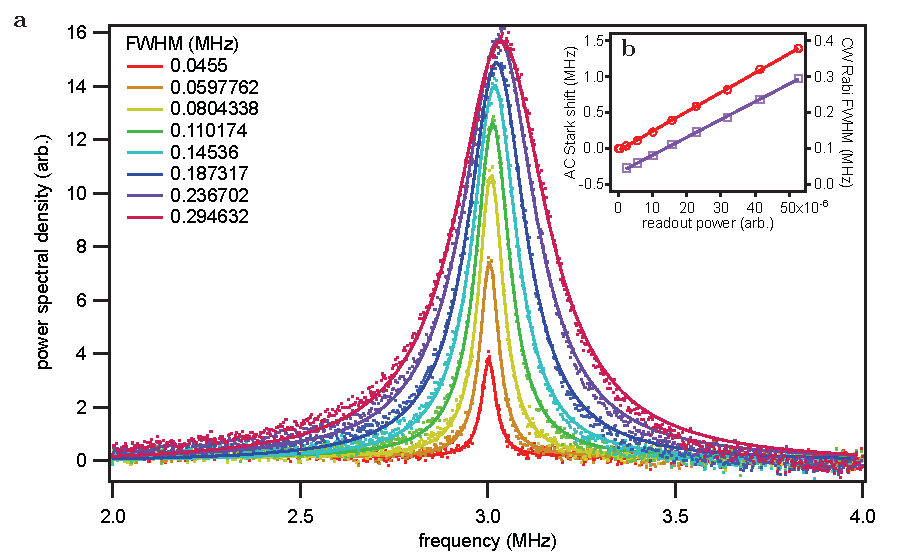
\includegraphics[width = 6in]{qfb_results_chapter/cw_rabi_and_gamma}
\end{center}
\caption[CW Rabi spectra and fits]{\textbf{a} CW Rabi spectra for a variety of measurement powers, from fairly weak measurement (red trace) to an optimal measurement power (magenta), and fits of the FWHM.  At the highest measurement power we observe a saturation in the height of the peak with increasing measurement strength.  This set of measurements was taken with a slightly odd paramp gain profile resulting in a sloping noise floor; this noise floor has been subtracted from the measured peaks for clarity and to improve the quality of the fits.  \textbf{b} AC stark shift (from Ramsey measurements, not shown; plotted in red, left axis) and the FWHM dephasing from \textbf{a} (plotted in purple, right axis), showing the linear relationship with measurement power.}
\label{fig:cw_rabi_and_gamma}
\end{figure*}

The purity of the qubit state in a single measurement can be revealed by averaging the ensemble in a different way.  Time-domain averaging for noisy oscillations will only work if the phase of the oscillations is essentially constant across every iteration of the experiment.  Instead, we can take the noisy experimental record from each individual experiment, convert it to a power spectrum using an FFT algorithm, and then average the power spectra together.  Korotkov calls this averaged power spectrum the \textit{CW Rabi spectrum}.  For high measurement efficiency and in the limit where the dephasing is dominated by the measurement, we should then clearly resolve a spectral peak corresponding to the measurement-dephased Rabi oscillations, centered at the Rabi frequency $\Omega_r$ and with a spectral width related to the total dephasing rate $\Gamma$ and a peak height above the noise floor related to the quantum efficiency $\eta$.  From reference \cite{korotkov_p2p}, the functional form of this peak is
\begin{equation}
S(\omega) = \frac{\Gamma \Omega_r^2 (\Delta V)^2}{(\omega^2 - \Omega_r^2)^2 + \Gamma^2 \omega^2}.
\end{equation}
The maximum occurs when $\omega = \Omega_r$ and has the value $S_{\rm max} = (\Delta V)^2 / \Gamma$.

Much of the most thorough CW Rabi spectrum data was taken in a cooldown prior to that corresponding to the published data set.  In this cooldown the measurement setup was not quite as well optimized as in the final data set, but the plots are illustrative so I will use them in this and the next section.  An example set of CW Rabi spectra are shown in Figure \ref{fig:cw_rabi_and_gamma}a.  For relatively weak measurement, the peak height is small.  As the measurement strength is increased, the peak height and width both grow due to the increased signal amplitude and measurement-induced dephasing rate.

Eventually, we reach an optimal measurement strength at which point increasing the magnitude of the signal does not increase the height of the peak.  This can be interpreted as an optimal trade-off between measurement accuracy and back-action.  Although the magnitude of the signal is increasing with increasing signal strength, the back-action of the measurement is broadening the peak such that even though the total power in the peak increases, the peak height remains fixed.  The slight rightward drift in the center frequency of the peaks is due to the power-dependent AC stark shift of the qubit which was not corrected for in this particular experiment.

\begin{figure*}
\begin{center}
	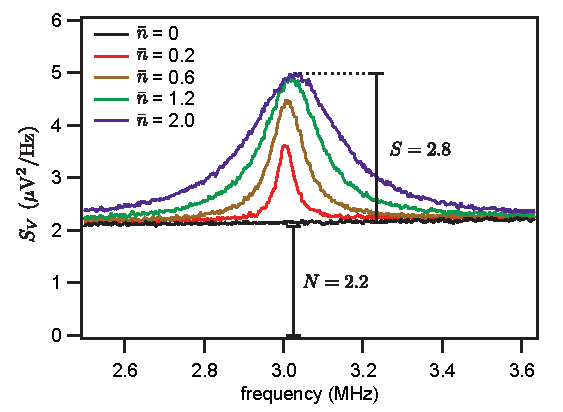
\includegraphics[width = 3.75in]{qfb_results_chapter/P2P}
\end{center}
\caption[Peak-to-pedestal ratio]{Measured CW Rabi spectra for several calibrated measurement powers, showing the saturation of the peak due to the measurement-disturbance tradeoff.  The ratio of the peak height to the noise floor provides a measurement of the total measurement efficiency $\eta$.}
\label{fig:P2P}
\end{figure*}

From \eqref{eq:bayesian_dephasing}, the spectral density of the noise floor of the CW Rabi spectrum for an ideal measurement is $S_0 = (\Delta V)^2 / 4 \Gamma_m$.  The ratio of the peak height to the noise floor (referred to as the \textit{peak-to-pedestal ratio} or \textit{P2P ratio} for short) is then calculated as $S_{\rm max} / S_0 = 4 \Gamma_m / \Gamma$.   From \eqref{eq:eta_basic_form}, we identify the ratio of dephasing rates as the quantum efficiency, allowing us to write $\rm P2P = 4 \eta$.  Thus, measuring the P2P ratio at the optimal measurement power described in the last paragraph provides another estimate of the total measurement efficiency $\eta$, complementing the Ramsey fringe technique discussed in section \ref{s:det_meas_eta}.  An example of this extraction is shown in Figure \ref{fig:P2P} with $\eta = S/4N = 0.32$ in this particular experiment.

\subsection{Quantum Zeno effect}

\begin{figure*}
\begin{center}
	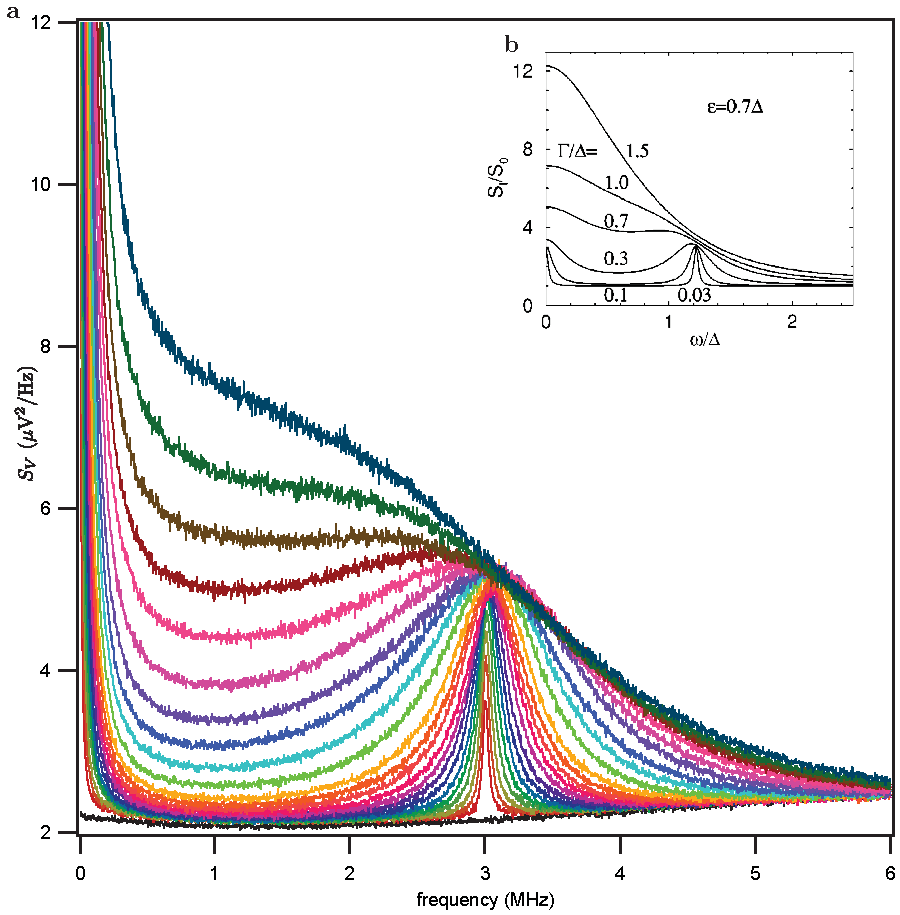
\includegraphics[width = 6in]{qfb_results_chapter/zeno}
\end{center}
\caption[CW Rabi spectrum and quantum Zeno effect]{\textbf{a} CW Rabi traces taken over a broad range of measurement strengths, smoothly covering the evolution from lightly-perturbed oscillations to telegraph-like measurement pinning of the qubit state.  \textbf{b} Theoretical curves for the same effect, showing beautiful qualitative agreement with the measured data.  Note that the parameter regime in this theory plot is not the same as that for the experimental data. In fact the parameters in the plot are described in the language for a quantum dot qubit read out with a quantum point contact, though the physics for the two systems is identical in the relevant regime.  Reproduced from reference \cite{korotkov_p2p}.}
\label{fig:zeno}
\end{figure*}

As seen in Figure \ref{fig:P2P}, the cavity photon number at which the measurement-disturbance tradeoff is saturated corresponds to a fairly small measurement power, whereas the power used for strong measurement is about 5 to 10 times larger.  What happens to the CW Rabi spectrum when the measurement is increased beyond the saturation point?  Qualitatively speaking, at some point the dephasing rate will exceed the Rabi frequency, and the qubit evolution will go from being something that looks like a noisy oscillation to something that looks mostly like random fluctuations with some weakly oscillating component.  There is no particular sharp transition which characterizes this changeover.

Measurements of the CW Rabi spectrum covering this entire regime are shown in Figure \ref{fig:zeno}.  At very strong measurement powers, the frequency of the peak begins to shift towards zero and becomes dramatically non-Lorentzian.  This transition from finite-frequency oscillations to a noisy spectrum centered at zero-frequency can be understood as an incarnation of the quantum Zeno effect.  Because the projective measurement time scale becomes short compared to the Rabi period, the strong measurement effectively pins the qubit state to one or the other eigenstate even though the dynamics of the system's free evolution should be oscillatory.

\subsection{Needles}

The aim of the feedback scheme is to stabilize the phase of the Rabi oscillations to that of some high-quality reference oscillator.  Or, equivalently, because phase fluctuations and small frequency fluctuations are interchangeable, we aim to stabilize the frequency of the Rabi oscillations to a precise value.  In the spectral domain, for a perfect reference oscillator, this type of oscillation corresponds to a $\delta$-function in frequency (any real oscillator will of course have a finite spectral width).  Thus, the signature of effective feedback control of the qubit is the appearance of a sharp, narrow peak on top of the CW Rabi spectrum.  Because the linewidth of the classical oscillator is sub-hertz and out experiments last for at most a millisecond or so, our FFT point spacing will always be larger than the width of this peak, implying that the signal in the experiment is literally one elevated point in the FFT.  Because of the extreme narrowness, we often refer to this peak as a \textit{needle}.

\begin{figure*}
\begin{center}
	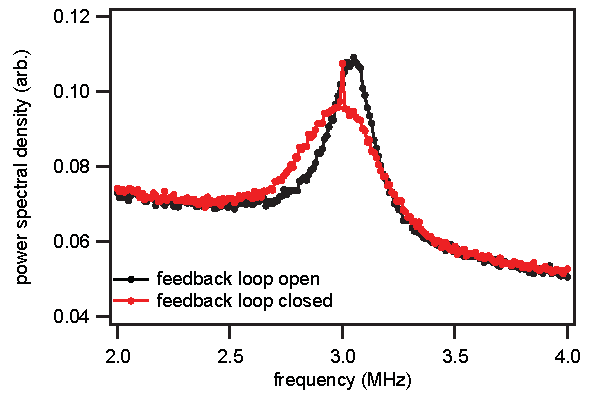
\includegraphics[width = 4in]{qfb_results_chapter/first_fb}
\end{center}
\caption[First observation of feedback stabilization]{The first confirmed feedback needle.}
\label{fig:first_fb}
\end{figure*}

Successful feedback was first measured on September 24, 2011, at about 5:30pm.  It was quite an exciting moment, not least of all because it was extremely unclear if we had really seen an effect at first.  The needle was barely visible above the top of the CW Rabi peak, and worse, because it is always exactly one point wide, it was difficult to determine if we were seeing a signal or just a small fluctuation in the noise.  After a bit of tuning of the feedback parameters, we were able to bring the needle conclusively above the peak.  The data taken at this moment are shown in Figure \ref{fig:first_fb}.  Cheers went up, ``quantum feedback!''

\begin{figure*}
\begin{center}
	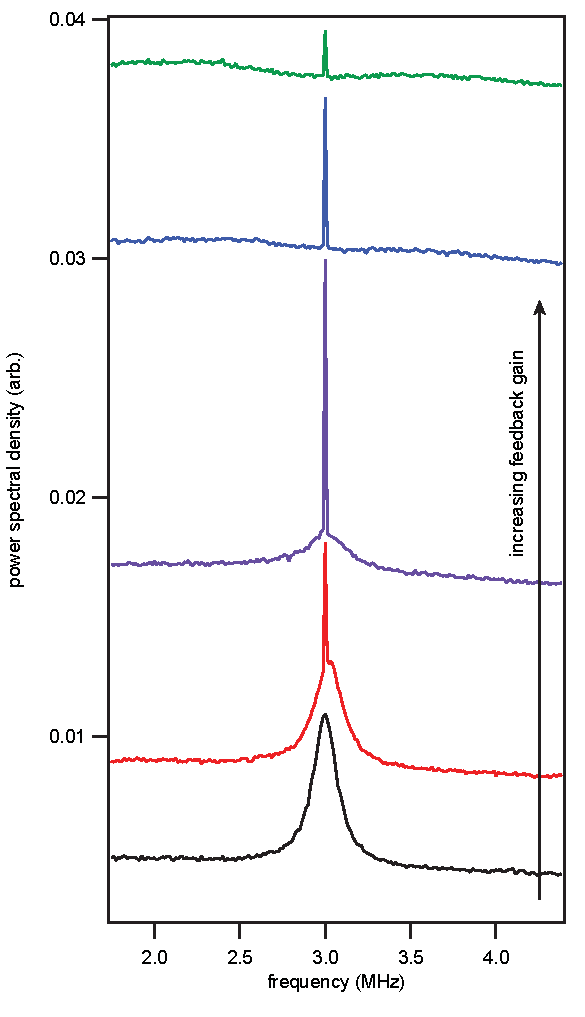
\includegraphics[width = 4in]{qfb_results_chapter/needle_zoo}
\end{center}
\caption[CW Rabi spectrum and needles versus feedback strength]{An assortment of CW Rabi spectra with feedback needles.  Each trace is taken with the same measurement power, with feedback strength increasing for each trace moving vertically up the plot, starting with no feedback in black.  Traces are offset for clarity.}
\label{fig:needle_zoo}
\end{figure*}

Because the needle has essentially zero spectral width while the CW Rabi spectrum itself is continuous, the needle can be more clearly observed by reducing the FFT point spacing, reducing the absolute power spectral density for every point except the needle.  A set of spectra with feedback from the final published data set are shown in Figure \ref{fig:needle_zoo}.  The black trace is taken with the feedback loop open.  The red trace shows a low feedback gain, where most of the oscillation power remains unsynchronized.  The purple trace represents the optimum feedback strength for this measurement power, with about half of the total Rabi peak power contained in the needle.  The blue and green traces show feedback gains which are above the optimum, where the feedback correction applied to the system is larger than the correction needed to undo the effect of the measurement dephasing.  In this regime, characteristic ``wings'' in the spectrum appear, particularly visible in the green trace.  This can be intuitively understood as the feedback ``oversteering'' the qubit oscillation frequency; the actual correction needed to stabilize the qubit is a relatively small frequency shift, but because the gain is large, the frequency correction becomes large, developing two peaks at a detuning proportional to the feedback gain.

\section{Time-domain measurements}

The needles alone are conclusive evidence of successful quantum feedback, and provide a complete quantitative picture of the feedback quality.  However, they do not impressively demonstrate the result because Rabi oscillations are not usually analyzed in the frequency domain.  Time domain measurements of the stabilized state viscerally demonstrate the feat accomplished in this experiment, because the time-domain equivalent of a needle is a \textit{coherent oscillation that does not decay}.  As long as the phase of the reference oscillator is stable with respect to the rest of the experiment, time-domain averaging is possible.

\begin{figure*}
\begin{center}
	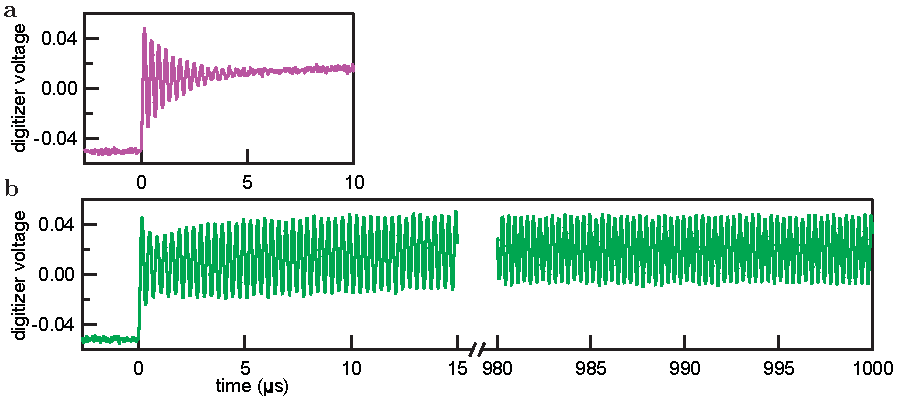
\includegraphics[width = 6in]{qfb_results_chapter/time_domain}
\end{center}
\caption[Stabilized time-domain Rabi oscillations]{\textbf{a} A typical averaged time-domain Rabi oscillation, showing the characteristic exponential decay associated with dephasing. \textbf{b}  Feedback-stabilized time domain Rabi oscillations.  Adapted from reference \cite{vijay_stabilizing_2012}.}
\label{fig:time_domain}
\end{figure*}

Time-domain-averaged Rabi oscillations are shown in Figure \ref{fig:time_domain}.  A weak measurement is constantly on, while the Rabi drive turns on at $t = 0$.  Figure \ref{fig:time_domain}a shows the typical exponentially-decaying oscillations for a qubit with a finite decoherence rate.  In this case, the dephasing is dominated by the measurement, so the oscillations decay relatively quickly.  Without a measurement, the oscillations decay on a timescale of about 10 $\mu$s.  In Figure \ref{fig:time_domain}b, the feedback loop is closed when the Rabi drive turns on.  The oscillations show an initial transient period while the qubit phase evolves to match that of the reference oscillator, and then stabilize to a finite contrast which does not decay in time.  The feedback efficiency is related to the contrast of the stabilized oscillations compared to the full-scale oscillations; the contrast here is about 50\%.  Here two measurements are stitched together, showing an initial 15 $\mu$s of stabilized oscillation, and another 20 $\mu$s after leaving the feedback loop closed for about 1 ms.  In this data, no post-selection has been done to remove the effect of thermal excitations out of the $ \{ \ket{0},\ket{1}\}$ manifold, which is visible as a slight upwards drift after the Rabi drive turns on.

\begin{figure*}
\begin{center}
	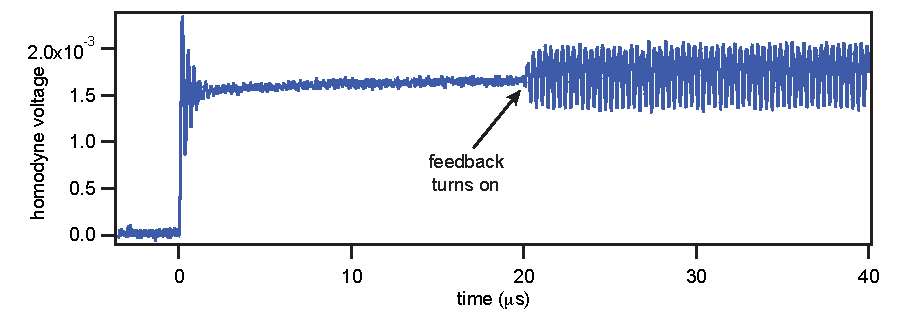
\includegraphics[width = 6in]{qfb_results_chapter/rephase}
\end{center}
\caption[Feedback re-phases a mixed state]{Time domain Rabi trace, showing the effect of delayed activation of the feedback control.  The  contrast is reduced compared to Figure \ref{fig:time_domain}b because this data was taken on a prior cooldown under different, less-optimized parameters.}
\label{fig:rephase}
\end{figure*}

Because the weak measurement extracts information about the phase of the qubit, the feedback stabilization will work regardless of the initial phase of the qubit oscillations.  Furthermore, because the feedback locking mechanism occurs in each individual iteration of the experiment, the feedback loop will still lock the oscillation phase even if the qubit's phase is completely randomized.  In other words, if we start with an ensemble of qubits in a completely mixed state, and then turn the feedback on, the ensemble will be re-cohered into a pure state (with a purity set by the feedback efficiency).  This effect is shown in Figure \ref{fig:rephase}, where we have delayed closing the feedback loop until 20 $\mu$s after the Rabi drive is turned on.

\section{Tomographic validation}

\begin{figure*}
\begin{center}
	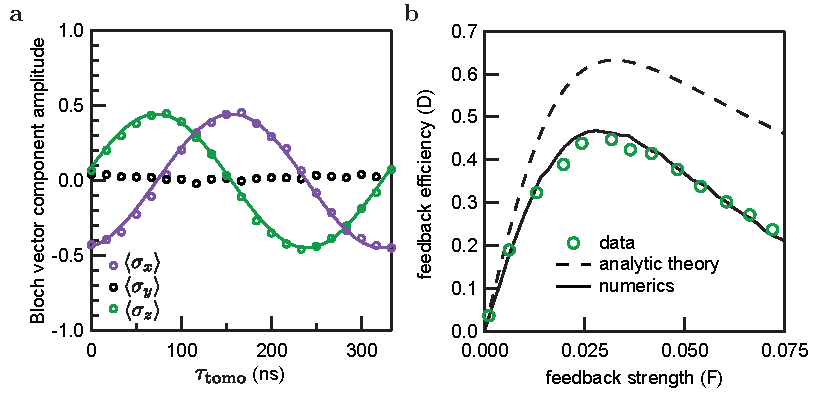
\includegraphics[width = 5.5in]{qfb_results_chapter/fb_tomo}
\end{center}
\caption[Tomographic validation of feedback]{\textbf{a} Tomographic validation of the feedback-stabilized qubit state, showing the measured Bloch vector components as a function of $\tau_\mathrm{tomo}$.  The Bloch vector components $\xpec{\sigma_x}$ and $\xpec{\sigma_z}$ are, as expected, sinusoidal oscillations with a $\pi/2$ phase shift, and an amplitude of 0.45, corresponding to a feedback efficiency $D = 0.45$.  The $\xpec{\sigma_y}$ component is essentially zero, as expected for driven Rabi oscillations in the $x-z$ plane.  \textbf{b} Tomographically-measured feedback efficiency $D$  versus feedback strength $F$.  The dashed line corresponds to the simple analytical theory, while the solid black line is based on numerical analysis including the effect of finite loop delay.  Adapted from reference \cite{vijay_stabilizing_2012}.}
\label{fig:fb_tomo}
\end{figure*}

In order to validate the quantum nature of the stabilized qubit state and precisely assess its purity, we stop the feedback after a time $(80 \ \mu\mathrm{s}) + \tau_\mathrm{tomo}$ and perform a complete tomographic reconstruction of the state of the qubit.  By repeating this experiment with a range of $\tau_\mathrm{tomo}$ covering one fully stabilized oscillation, we can fit the resulting reconstruction of the Bloch vector components to sinusoids and extract the feedback efficiency $D$ as the length of the Bloch vector.  By repeating this experiment for a variety of feedback and measurement strengths, we can find the best global performance of the feedback.  Tomographic reconstruction of a feedback-stabilized oscillation is shown in Figure \ref{fig:fb_tomo}a for the experimentally-determined optimal conditions $\bar{n} = 0.47$ (corresponding to a measurement-induced dephasing rate $\Gamma_\varphi/2\pi = 134$ kHz) and $F = 0.032$.  The reconstructed state is a coherent oscillation in the $x-z$ plane at the Rabi frequency with a Bloch vector length of 0.45, corresponding to $D = 0.45$.

In order to compare these results to the theoretical prediction for the feedback efficiency, we examine the dependence of the efficiency on the feedback gain $F$, shown in Figure \ref{fig:fb_tomo}b.  The efficiency quickly rises as the feedback strength is turned up, peaks, and then more gently slopes back down as the feedback correction being applied to the system becomes too large.  Plotted along with the data are the predictions for the simple analytic result
    \begin{equation}
    D=2 \left(\displaystyle \frac{1}{\eta}\, \frac{F}{\Gamma/\Omega_0}
+\frac{\Gamma/\Omega_0}{F} \right)^{-1}
    \end{equation}
as well as the results of a complete numerical calculation which includes the effect of the finite loop delay, using the measured efficiency $\eta = 0.4$ and the total dephasing rate $\Gamma/2 \pi = 154$ kHz.  Details on the numerical calculation can be found in the supplementary information of reference \cite{vijay_stabilizing_2012}.























\chapter{JTWPA theory}
\label{c:twpa_theory}

The theoretical treatment of the Josephson traveling-wave parametric amplifier (JTWPA) has gone through several iterations, starting with relatively back-of-the-envelope calculations and evolving into a very complete description of the full nonlinear behavior of the device, including multiple non-idealities corresponding to the reality of the physical implementation.  I will begin this chapter with a discussion of the basic problem of phase matching in nonlinear optical devices as well as the general theory of four-wave mixing.  Next, I will lay out a rigorous theory of the JTWPA, and then describe our solution to the phase matching problem and exactly solve the dispersion relation using a standard technique from microwave network analysis.  Finally, I will present theoretical predictions for the amplifier gain, bandwidth, and input compression power.

\section{Nonlinear refraction, phase modulation, and four-wave mixing}

The language of circuit theory is appropriate to describe the behavior of lumped-element microwave networks, including lumped nonlinearities such as transistors and Josephson junctions.  Distributed networks generally consist of series of linear waveguides and lumped element components.  The literature of microwave networks in general does not treat the case of propagation in nonlinear waveguides; this is largely because high-quality, highly nonlinear, lumped-element components are commonplace in microwave electronics and are relatively straightforward to model.  At optical frequencies, however, the wavelength is so small that virtually every component in the system must be treated in the distributed limit, and thus a rich theory of continuum nonlinear wave propagation has been developed to model nonlinear optical systems.  The junction-loaded transmission line which comprises the JTWPA can be considered in this regime, as the lumped elements are in the deep-subwavelength limit and the transmission line is well approximated as a continuum.  Thus, it is natural to introduce the language of continuum nonlinear optics, and apply this existing rich theory to understand the behavior of the JTWPA.  In this section I will briefly introduce a few of the fundamental physical effects present in nonlinear optical systems, following chapters 1 and 10 of reference \cite{Agrawal2012}.  This section will be expressed in the language of single spatial mode optics, which is essentially analogous to the microwave case except for the additional polarization degree of freedom present in the optical case.

For a purely linear dielectric medium, we can write the polarization vector $\vec{P}$ of the material as
\begin{equation}
\vec{P} = \epsilon_0 \boldsymbol{\chi} \cdot \vec{E}
\end{equation}
where $\boldsymbol{\chi}$ is the material susceptibility.  In general, the polarization response of any material will become nonlinear if $|\vec{E}|$ is made large enough.  In that case, we can express the material polarization vector as a series expansion in increasing orders of $\vec{E}$
\begin{equation}
\vec{P} = \epsilon_0 \left( \boldsymbol{\chi}^{(1)} \cdot \vec{E} + \boldsymbol{\chi}^{(2)} : \vec{E}\vec{E} + \boldsymbol{\chi}^{(3)}\mathbin{\vdots} \mathbf{EEE}+ \cdots \right)
\label{eq:P_NL}
\end{equation}
where $\boldsymbol{\chi}^{(j)}$ is the $j$th order susceptibility (a rank $j+1$ tensor) and the vertical dots indicate tensor multiplication.  The second order susceptibility $\boldsymbol{\chi}^{(2)}$ vanishes for a material with spatial inversion symmetry, which will hold for our nonlinear junction-loaded transmission line.  Thus, $\boldsymbol{\chi}^{(3)}$ is the first nonlinear order to contribute, and it is this term that brings about virtually all nonlinear effects of interest, including the four-wave mixing process used in parametric amplification.

Though $\boldsymbol{\chi}^{(3)}$ is a rank-four tensor, we are only interested in one component of that tensor, the nonlinear index of refraction
\begin{equation}
n_2 = \frac{3}{8n} \textrm{Re}(\chi^{(3)}_{xxxx}).
\end{equation}
This term involves no mixing between polarization states of the electric field.  Since our microwave system lacks a polarization degree of freedom anyway, we can lump all of the effect of the $\boldsymbol{\chi}^{(3)}$ nonlinearity into this one number.  This allows us to write a simple form for the nonlinear index of refraction as
\begin{equation}
\tilde{n}(|E|^2) = n + n_2 |E|^2
\end{equation}
where $|E|^2$ is the optical intensity.  The phase of a wave that propagates through this medium for a length $L$ evolves as
\begin{equation}
\phi = \tilde{n} k_0 L = (n + n_2 |E|^2)k_0 L
\end{equation}
where $k_0 = 2\pi/\lambda$.  We can re-express this equation as the sum of two terms
\begin{equation}
\phi = \varphi_{0} + \phi_{\textrm{NL}} = n k_0 L + n_2 k_0 L |E|^2;
\end{equation}
the first term is the familiar linear phase shift, while the second term is known as \textit{self-phase modulation} (SPM) as the wave generates in itself an extra intensity-dependent phase shift.

What about a case where we have more than one wave co-propagating in this nonlinear medium?  Assuming the two waves have the same polarization, the total electric field can be written as
\begin{equation}
E = \frac{1}{2} ( E_1 e^{-i \omega_1 t} + E_2 e^{-i \omega_2 t} + \textrm{c.c.}).
\end{equation}
We plug this equation into the expression for $\phi_{\textrm{NL}}$ and neglect terms rotating at any frequency besides $\omega_1$ and $\omega_2$; the resulting nonlinear phase shift for the wave at $\omega_1$ is
\begin{equation}
\phi_{\textrm{NL}} = n_2 k_0 L ( |E_1|^2 + 2 |E_2|^2).
\end{equation}
We identify the first term as the same SPM effect we found for single-wave propagation.  The second term is now a phase shift induced in the wave at $\omega_1$ by the wave at $\omega_2$ and known as \textit{cross-phase modulation} (XPM).  Compensating these nonlinear phase shifts will be the primary challenge in realizing efficient four-wave mixing in a traveling-wave amplifier.

The physical origin of four-wave mixing is the nonlinear dependence on the electric field in the $\boldsymbol{\chi}^{(3)}$ term of (\ref{eq:P_NL}).    For four waves of the same polarization oscillating at $\omega_j$ where $j \in \{1,2,3,4\}$, we can write the total electric field as
\begin{equation}
E = \frac{1}{2} \sum^4_{j=1} E_j \exp{[i (k_j z - \omega_j t)]} +  \textrm{c.c.}
\label{eq:E_series}
\end{equation}
where the propagation constant $k_j = \tilde{n}_j \omega_j / c$ and $\tilde{n}_j$ is the nonlinear index of refraction for mode $j$.  Substituting this form into (\ref{eq:P_NL}), we find a large number of terms involving the product of three electric fields.  If we express the result as a series in the same form as (\ref{eq:E_series}), we can for instance express the total material polarization oscillating at $\omega_4$ as
\begin{align}
P_4 &= \frac{3 \epsilon_0}{4} \chi^{(3)}_{xxxx} [ |E_4|^2 E_4 + 2 (|E_1|^2 + |E_2|^2 + |E_3|^2)E_4 \notag \\
&+2E_1 E_2 E_3 \exp{(i \Theta_+)} + 2 E_1 E_2 E_3^* \exp{(i \Theta_-)} + \hdots]
\label{eq:fwm_prods}
\end{align}
where $\Theta_+$ and $\Theta_-$ are defined as
\begin{align}
\Theta_+ &= (k_1 + k_2 + k_3 - k_4)z - (\omega_1 + \omega_2 + \omega_3 - \omega_4)t,
\\ \Theta_- &= (k_1 + k_2 - k_3 - k_4)z - (\omega_1 + \omega_2 - \omega_3 - \omega_4)t.
\end{align}

We can immediately identify the term proportional to $|E_4|^2 E_4$ as SPM, and the term following it as XPM.  The remaining two terms are proportional to sum and difference frequency combinations of the waves.  When $\Theta_{\pm}$ have a nonzero value, the latter terms in \eqref{eq:fwm_prods} are oscillatory and cannot build up a large effect over the length of the device; however, when $\Theta$ is close to zero, they can contribute at the same order as the SPM and XPM terms.  In this regime these frequency-mixing terms can contribute a large effect to the total nonlinear propagation and create significant exchanges of energy in length, realizing an efficient multi-wave mixing process.

The term containing $\Theta_+$ expresses energy conservation of the form
\begin{equation}
\omega_4 = \omega_1 + \omega_2 + \omega_3
\end{equation}
where three photons combine to produce one photon.  This process is responsible for effects such as third-harmonic generation when $\omega_1 = \omega_2 = \omega_3$.  The term containing $\Theta_-$, on the other hand, destroys two photons while creating two photons, such that
\begin{equation}
\omega_3 + \omega_4 = \omega_1 + \omega_2.
\end{equation}
We are primarily interested in the case of degenerate four-wave mixing, where $\omega_1 = \omega_2$.  For this process to not be oscillatory in space, we require the satisfaction of the condition $\Delta k = 0$ where
\begin{equation}
\Delta k = k_3 + k_4 - k_1 - k_2.
\end{equation}
The propagation constants $k_j$ are themselves dependent on frequency through the dispersion relation $k(\omega)$ and also to the total field intensity through $\tilde{n}_j$.







\section{Derivation of the continuum wave equation for the JTWPA}\label{s:twpa_wave_eq}

In order to link to the continuum nonlinear optical theory developed in the last section, we need to find a continuum description of the lumped-element nonlinear transmission line forming the heart of the JTWPA.  The original derivation of the continuum nonlinear wave equation for the JTWPA was performed by Friedland and Yaakobi in our publication in Physical Review Letters \cite{Yaakobi:2013kx}.  The circuit model for a unit cell of the junction-loaded transmission line is shown in Figure \ref{fig:TWPA_circuit_model}. The basic idea is to apply Kirchoff's laws to one unit cell and its neighbors, use the translational symmetry of the transmission line to create a discrete wave equation, and then find the continuum approximation by converting finite difference relations to derivatives.

\begin{figure*}
\begin{center}
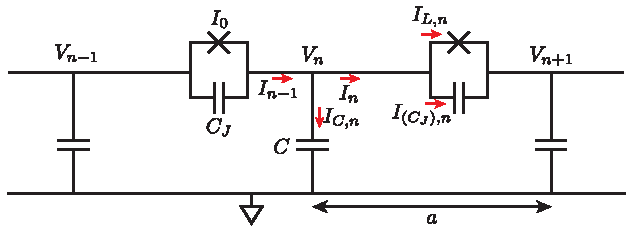
\includegraphics[width=4.2in]{twpa_theory/TWPA_circuit_model}
\end{center}
\caption[Circuit model for junction-loaded transmission line]{Circuit model for junction-loaded transmission line.  The bottom wire is connected to ground, and the conventions for voltage drop and current flow are indicated.}
\label{fig:TWPA_circuit_model}
\end{figure*}


Current conservation at each node implies
\begin{equation}
I_{n}=I_{ (C_{J}), n}+I_{L,n}.  \label{Current conservation secondary}
\end{equation}
The current in capacitor $C_{J}, n$ is related to the voltages $V_{n}$ and $V_{n+1}$\ by the derivative 
\begin{equation}
I_{ (C_{J}), n}=-C_{J}\frac{d}{dt}\left( V_{n+1}-V_{n}\right).
\label{Current voltage cj}
\end{equation}
We define the magnetic flux as the time integral of the voltage across the inductor, expressed here as a difference equation 
\begin{equation}
V_{n+1}-V_{n}=-\frac{d\Phi _{n}}{dt},
\label{Magnetic flux definition}
\end{equation}
and we write the expression for the junction current-phase relation 
\begin{equation}
I_{L,n}=I_{0}\sin \left[ \frac{\Phi _{n}}{\varphi_{0}}\right] ,
\label{Josephson current}
\end{equation}
where $\varphi_{0} = \Phi _{0}/2\pi$ is the reduced flux quantum.  Differentiation of the last equation yields
\begin{equation}
\frac{dI_{L,n}}{dt}=\frac{I_{0}}{\varphi_{0}}\left( \cos \left[ \frac{\Phi _{n}}{\varphi_{0}}\right] \right) \frac{d\Phi _{n}}{dt}.
\end{equation}
Then
\begin{equation}
\frac{d\Phi _{n}}{dt}=\frac{dI_{L,n}}{dt}\frac{\varphi_{0}}{I_{0}}\left( 1-\sin ^{2}\left[ \frac{\Phi _{n}}{\varphi_{0}}\right] \right)^{-\frac{1}{2}},
\end{equation}
which, upon using Eq. (\ref{Josephson current}), becomes
\begin{equation}
\frac{d\Phi _{n}}{dt}=\frac{\varphi_{0}}{I_{0}}\left( 1-\left[ \frac{I_{L,n}}{I_{0}}\right] ^{2}\right) ^{-\frac{1}{2}}\frac{dI_{L,n}}{dt}.
\label{Nonlinear inductance}
\end{equation}
For the weakly nonlinear regime $I_{L,n}/I_{0} \ll 1$, we approximate the nonlinear contribution to first order as
\begin{equation}
\frac{d\Phi _{n}}{dt}=\frac{\varphi_{0}}{I_{0}}\left( 1+\frac{1}{2} \left[ \frac{I_{L,n}}{I_{0}}\right] ^{2}\right) \frac{dI_{L,n}}{dt}.
\label{Weak nonlinear inductance}
\end{equation}
Since the current through capacitor $C_n$ is
\begin{equation}
I_{C,n}=-C \frac{d}{dt}\left( 0-V_{n}\right)=C\frac{dV_{n}}{dt},
\label{Capacitor current}
\end{equation}
current conservation yields
\begin{equation}
I_{n}-I_{n-1}=-C\frac{dV_{n}}{dt}.
\label{Current voltage primary}
\end{equation}
Next, we use equations 
(\ref{Magnetic flux definition}) and (\ref{Weak nonlinear inductance}) to get
\begin{equation}
V_{n+1}-V_{n}=-L\frac{dI_{L,n}}{dt}-\frac{\varphi_{0}}{6I_{0}^{3}}\frac{d}{dt}\left( I_{L,n}\right) ^{3},  \label{B}
\end{equation}
where $L=\varphi_{0}/I_{0}.$ Introducing the node fluxes $\phi_{n}$ as
\begin{equation}
V_{n}\equiv \frac{d\phi_{n}}{dt}
\label{node flux definition}
\end{equation}
and integrating (\ref{B}), we obtain
\begin{equation}
\phi_{n+1}-\phi_{n}=-LI_{L,n}-\frac{L}{6I_{0}^{2}}I_{L,n}^{3}
\label{V_n difference}
\end{equation}
where we have set the integration constant to zero. Rearranging the last equation yields
\begin{equation}
I_{L,n}=-\frac{1}{L}\left( \phi_{n+1}-\phi_{n}\right) -\frac{1}{6I_{0}^{2}}I_{L,n}^{3}.
\end{equation}
Assuming that the nonlinear term is small, we can approximate this to lowest (linear) order 
\begin{equation}
I_{L,n}\approx -\frac{1}{L}\left( \phi_{n+1}-\phi_{n}\right) .
\end{equation}
Then, by plugging this expression back into \eqref{V_n difference}, we get the first-order nonlinear approximation
\begin{equation}
I_{L,n}=-\frac{1}{L}\left( \phi_{n+1}-\phi_{n}\right) + \frac{1}{6I_{0}^{2}L^{3}}\left( \phi_{n+1}-\phi_{n}\right) ^{3}.  \label{I_Ln second iteration}
\end{equation}
Finally, combining equations (\ref{Current conservation secondary}), (\ref{Current voltage cj}), (\ref{Current voltage primary}), (\ref{node flux definition}) and (\ref{I_Ln second iteration}), we obtain the first-order nonlinear system
\begin{align}
-C \frac{d^{2}\phi_{n}}{dt^{2}} = &-C_{J}\frac{d^{2}}{dt^{2}}\left[ \phi_{n+1}+\phi_{n-1}-2 \phi_{n}\right]  \notag \\
&-\frac{1}{L}\left[ \phi_{n+1}+\phi_{n-1}-2 \phi_{n}\right]  \notag \\
&+\frac{1}{6I_{0}^{2}L^{3}}\left[ \left( \phi_{n+1}-\phi_{n}\right) ^{3}-\left( \phi_{n}-\phi_{n-1}\right) ^{3}\right].
\label{Discrete wave equation uniform}
\end{align}

At this point we could numerically solve this equation for an arbitrary number of unit cells, but this does not provide any further intuition.  We would like to make a link to the existing theory of continuum nonlinear optics; if we assume that the wavelength of a propagating mode is much larger than one unit cell ($a/\lambda \ll 1$), we can replace the discrete $n$ by a continuous position $x$ and replace the finite differences in the discrete equations by their continuous counterparts to second order in $(a/\lambda)$: 
\begin{align}
\phi_{n+1}-\phi_{n} &\approx a\frac{\partial \phi}{\partial x}+\frac{1}{2}a^{2}\frac{\partial ^{2} \phi}{\partial x^{2}} \\
\phi_{n}-\phi_{n-1} &\approx a\frac{\partial \phi}{\partial x}-\frac{1}{2}a^{2}\frac{\partial ^{2}\phi}{\partial x^{2}}
\end{align}
\begin{equation}
\phi_{n+1}+\phi_{n-1} -2\phi_{n} \approx a^{2}\frac{\partial ^{2}\phi}{\partial x^{2}}.
\end{equation}
Then, to lowest significant order in $a/\lambda$,
\begin{equation}
\left( \phi_{n+1}-\phi_{n}\right) ^{3}-\left( \phi_{n}-\phi_{n-1}\right) ^{3}\approx 3a^{4}\left( \frac{\partial ^{2}\phi}{\partial x^{2}}\right) \left( \frac{\partial \phi}{\partial x}\right) ^{2},
\end{equation}
and we arrive at the continuous counterpart of (\ref{Discrete wave equation uniform}):
\begin{equation}
C\frac{\partial ^{2}\phi}{\partial t^{2}}-\frac{a^{2}}{L} \frac{\partial ^{2}\phi}{\partial x^{2}}-C_{J}a^{2}\frac{\partial ^{4}\phi}{\partial t^{2}\partial x^{2}}+\frac{a^{4}}{2I_{0}^{2}L^{3}}\left( \frac{\partial^{2}\phi}{\partial x^{2}}\right) \left( \frac{\partial \phi}{\partial x}\right)^{2}=0.
\end{equation}
The first three terms in this expression describe weakly dispersive linear waves, while the fourth term represents the nonlinearity due to the junctions.

\section{Efficient parametric amplification}

With the continuum wave equation for the JTWPA in hand, we can attempt to find an approximate analytical solution for the behavior of several coupled waves.  This derivation is analogous to the technique used in nonlinear optics, described in chapter 10 of reference \cite{Agrawal2012}; the only major differences for this system are the presence of the weakly dispersive term due to the junction self-capacitance, and the simplicity of a purely one-dimensional problem.  This calculation was performed by Kevin O'Brien and appears as Appendix 1 in our publication in Physical Review Letters \cite{OBrien2014}.  I reproduce the full details of this calculation in Appendix \ref{a:twpa_paramp}.

By making the ansatz that the solutions are traveling waves, taking the slowly varying envelope approximation, and neglecting pump depletion (that is, assuming the energy of the pump wave remains constant over the length of the transmission line), we obtain a set of coupled wave equations which describe the energy exchange between the pump, signal, and idler:
\begin{align}
\frac{{\partial {a_s}}}{{\partial x}} - i{\kappa _s}a_i^*{e^{i(\Delta {k_L} + 2{\alpha _p} - {\alpha _s} - {\alpha _i})x}} &= 0 \label{eq:1} \\
\frac{{\partial {a_i}}}{{\partial x}} - i{\kappa _i}a_s^*{e^{i(\Delta {k_L} + 2{\alpha _p} - {\alpha _s} - {\alpha _i})x}} &= 0 \label{eq:2}
\end{align}
where $a_s$ and $a_i$ are the slowly-varying signal and idler amplitudes, $\Delta {k_L} = 2{k_p} - {k_s} - {k_i}$ is the phase mismatch in the low pump power limit, and the coupling factors $\alpha_p$, $\alpha_s$, and $\alpha_i$ represent the change in the wave vector of the pump, signal, and idler due to SPM and XPM induced by the pump. The coupling factors depend on the circuit parameters and scale quadratically with the pump current. The lack of an equivalent equation for the spatial variation of $a_p$ is explicitly due to the undepleted pump approximation.

Maximum parametric gain is achieved when the exponential terms are constant, rather than oscillating, implying that the phase mismatch $\Delta k = \Delta {k_L} + 2{\alpha _p} - {\alpha _s} - {\alpha _i}$ must then be zero. The coupled wave equations (\ref{eq:1}), (\ref{eq:2}) are similar to the coupled amplitude equations for an optical parametric amplifier \cite{armstrong_interactions_1962} and have the solution
\begin{equation}
{a_s}(x) = {a_s}(0)\left( {\cosh gx - \frac{{i\Delta k}}{{2g}}\sinh gx} \right){e^{i\Delta kx/2}} \label{eq:5}
\end{equation}
with the gain coefficient
\begin{equation}
g=\sqrt{\kappa_s \kappa^*_i -(\Delta k/2)^2}.
\label{eq:g}
\end{equation}
For $a_i(0) = 0$ and perfect phase matching $\Delta k = 0$, this expression implies exponential gain, $a_s(x) \approx a_s(0)e^{gx}/2$. For poor phase matching $g$ is imaginary and the power gain scales quadratically with length rather than exponentially. 

With a purely linear dispersion relation $k(\omega) \propto \omega$, the parametric process is phase matched at zero pump power, but rapidly loses phase matching as the pump power increases due pump power dependence in the coupling coefficients $\alpha$.  If we neglect the small dispersion due to $C_J$ and the small frequency dependence of the wave impedances, the exact expression for the phase mismatch \eqref{eq:a21} can be simplified to yield
\begin{equation}
\Delta k \approx 2k_p-k_s-k_i - 2{k_p}\kappa,
\label{eq:deltak}
\end{equation}
where
\begin{equation}
\kappa  = \frac{a^2 k_p^2 \left| Z \right|^2}{16 L^2 \omega _p^2} \left( \frac{I_p}{I_0} \right)^2.
\label{eq:kappa}
\end{equation}
We have now arrived at the central challenge of building a practical amplifier: satisfying the phase matching condition to achieve exponential gain.  We can see from the form of (\ref{eq:deltak}) that as the pump power increases, $\Delta k$ becomes negative.  Thus, to compensate this effect, we could either decrease $k_s$ and $k_i$ or increase $k_p$, as $\kappa$ is generally much smaller than unity.  Because we aim to realize a broadband amplifier and $\omega_s$ is not fixed, it makes more sense to attempt to locally modify the dispersion relation near $\omega_p$ to increase $k_p$.




\section{Dispersion relation and resonant phase matching}

To derive the small-signal dispersion relation $k(\omega)$ of the JTWPA, I will employ a standard formalism from microwave engineering called the \textit{ABCD matrix} formalism, described in chapter 4 of reference \cite{pozar1997microwave}.  The ABCD matrix, also known as the transmission matrix, is quite useful in this situation as cascading several 2-port microwave networks is equivalent to taking the product of their ABCD matrices.  This formalism is somewhat more heavyweight than required for the following calculation, but it applies nicely to more complex cases such as the cascade of several dissimilar unit cells forming a supercell which is then repeated.  It is also straightforward to numerically compute the dispersion relation for a finite rather than infinite line in this formalism using matrix multiplications.

For an arbitrary 2-port network with input voltage $V_{in}$ and input current (flowing into port 1) $I_{in}$, we can express the output voltage $V_{out}$ and output current (flowing out of port 2) $I_{out}$ as the product of a 2 $\times$ 2 matrix, creatively named the ABCD matrix:
\begin{equation}
\left( \begin{array}{c}
V_{out} \\
I_{out} \end{array} \right) =
\left( \begin{array}{cc}
A & B \\
C & D \end{array} \right)
\left( \begin{array}{c}
V_{in} \\
I_{in} \end{array} \right)
\label{eq:genABCD}
\end{equation}

For a reciprocal network, $AD-BC = 1$.  For a lossless, reciprocal network, $A$ and $D$ are real while $B$ and $C$ are imaginary.  For a transmission line formed from an infinite chain of repeated unit cells of physical length $a$, we can derive the dispersion relation by imposing translation symmetry on the input and output voltages of a single unit cell
\begin{equation}
\left( \begin{array}{c}
V_{out} \\
I_{out} \end{array} \right) =
e^{ika}
\left( \begin{array}{c}
V_{in} \\
I_{in} \end{array} \right).
\label{eq:transsym}
\end{equation}
Combined with (\ref{eq:genABCD}) we now have an eigenvalue problem wherein a solution must satisfy
\begin{equation}
\det
\left( \begin{array}{cc}
A - e^{-ika} & B \\
C & D - e^{ika} \end{array} \right)
= 0.
\label{eq:eig}
\end{equation}
For a reciprocal network we know that $AD-BC=1$, which reduces this relation to the very simple form
\begin{equation}
A + D = 2 \cos(ka).
\label{eq:disp}
\end{equation}
$A$ and $D$ will include factors of $\omega$ from the various impedances in the network, so this is the dispersion relation of the transmission line.

\begin{figure*}
\begin{center}
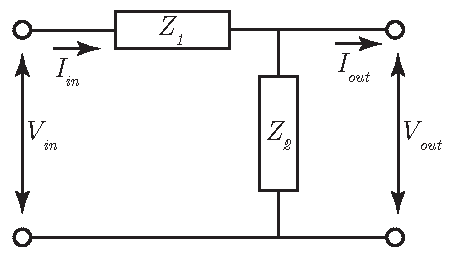
\includegraphics[width=3in]{twpa_theory/series_and_shunt_Z_network}
\end{center}
\caption[Generic series and shunt impedance network]{General two-port network under consideration, with one series impedance $Z_1$ and one shunt impedance $Z_2$.  Note current and voltage conventions.}
\label{fig:Znet}
\end{figure*}

We can easily derive the ABCD matrix for the general network shown in Fig. \ref{fig:Znet} using Kirchoff's laws.  This network is general enough to cover lots of interesting cases.  The voltage and current at the output are
\begin{equation}
V_{out} = V_{in} - I_{in} Z_1
\label{eq:volt}
\end{equation}
\begin{equation}
I_{out} = I_{in} - V_{out}/Z_2 = (-1/Z_2)V_{in} + (1 + Z_1/Z_2) I_{in}
\label{eq:curr}
\end{equation}
so the ABCD matrix of this network is
\begin{equation}
\left( \begin{array}{cc}
1 & -Z_1 \\
-1/Z_2 & 1+Z_1/Z_2 \end{array} \right).
\label{eq:2ZABCD}
\end{equation}
Thus, from (\ref{eq:disp}), for arbitrary series and shunt impedances the dispersion relation of this network is
\begin{equation}
ka = \cos^{-1}(1 + Z_1/2Z_2).
\label{eq:twoZdisp}
\end{equation}
For a simple LC ladder transmission line, $Z_1 = i \omega L$ and $Z_2 = 1/i \omega C$ so the dispersion relation is
\begin{equation}
ka = \cos^{-1}\left(1 - \frac{\omega^2}{(2 \omega_0)^2}\right),
\label{eq:LC_ladder_disp}
\end{equation}
where $\omega_0 = 1/\sqrt{LC}$.  A plot of this equation is shown as the red trace in Figure \ref{fig:JJ_ladder_disp}, in normalized units.  The characteristic frequency $\omega_0$ is called the \textit{plasma frequency} of the transmission line, corresponding to the resonance frequency of each rung of the LC ladder.  Above twice the plasma frequency, the dispersion relation is imaginary and there is no solution to the wave equation that permits a traveling mode, implying the existence of a very opaque stop-band above $2\omega_0$.  At frequencies much smaller than $\omega_0$, the dispersion relation is well-approximated as linear.

\begin{figure*}
\begin{center}
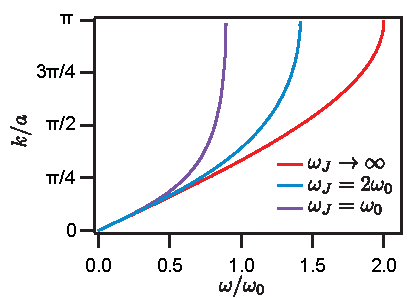
\includegraphics[width=2.75in]{twpa_theory/JJ_ladder_disp}
\end{center}
\caption[Dispersion relation for small-signal junction-loaded transmission line]{Dispersion relations for various ratios of plasma frequencies.  The case where the inductance has no parallel capacitance is plotted in red.  As the junction plasma frequency is reduced (finite shunt capacitance across the inductor), the cutoff frequency decreases and the curvature of the band increases.}
\label{fig:JJ_ladder_disp}
\end{figure*}

For the junction-loaded transmission line from Figure \ref{fig:TWPA_circuit_model}, the Josephson inductance is shunted by the intrinsic capacitance of the junction, so $Z_1$ is the parallel combination of $Z_L$ and $Z_{C_j}$.  This leads to a slightly more complex form
\begin{equation}
ka = \cos^{-1}\left(1 - \frac{\omega^2}{2 \omega_0^2 (1 - \omega^2/\omega_J^2)}\right)
\label{eq:JJ_ladder_disp}
\end{equation}
where we have introduced another characteristic frequency $\omega_J = 1/\sqrt{L C_J}$, the plasma frequency of the Josephson junction.  The net effect on the dispersion relation is to introduce an additional curvature into the band, and also modify the location of the edge of the stop band.  The cutoff frequency is now given by
\begin{equation}
\omega_C = \frac{2 \omega_0}{\sqrt{1 - 4 \omega_0^2/\omega_J^2}}.
\label{eq:JJ_disp_cutoff}
\end{equation}
In the small-signal regime, the phase matching condition $2 k_p = k_s + k_i$ will be satisfied for a perfectly linear dispersion.  The curvature of the band introduced by the two plasma frequencies serves to spoil this linearity for frequencies at an appreciable fraction of the cutoff frequency, and it is this band curvature that will be partially responsible for determining the amplification bandwidth of the JTWPA.

It is at this point that we must determine some method to create a local modification in the dispersion relation to satisfy (\ref{eq:deltak}).  There are many techniques known in nonlinear optical system to accomplish this \cite{armstrong_interactions_1962,Agrawal2012}; however, all of those systems are generally faced with the constraint of a very short optical wavelength, requiring schemes that work on the basis of distributed geometry.  Because the JTWPA is a microwave metamaterial and is already composed of deep-subwavelength elements, we can take a completely different and new approach to the problem.

\begin{figure*}
\begin{center}
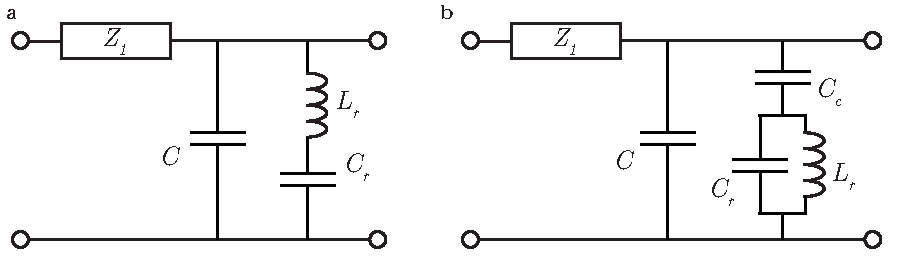
\includegraphics[width=6in]{twpa_theory/shunt_resonators}
\end{center}
\caption[Shunt resonator topologies]{Shunt resonator topologies: \textbf{a} series LC shunt; \textbf{b} capacitively-coupled parallel LC shunt.}
\label{fig:shuntres}
\end{figure*}

Because we seek a narrowband modification to the dispersion relation, we can start with the most common narrowband circuit topology: a resonator.  The most straightforward way to add a resonance is the addition of a series LC resonator in parallel with the capacitance to ground as shown in Figure \ref{fig:shuntres}a.  This configuration can be understood as a common circuit topology for implementing a notch filter.  Nearby but outside the stop-band of this filter the linear wave propagation will be slightly altered, leading to an increase in wavevector.  An alternative to the series LC shunt resonator is to add a capacitvely-coupled parallel LC resonator, shown in Figure \ref{fig:shuntres}b.  By introducing the coupling capacitor $C_c$, this topology has an extra degree of freedom compared to the series LC resonator, allowing the impedance of the resonator and the coupling to the transmission line to be adjusted independently.  This extra freedom will turn out to be crucial in fabricating a realistic device, so we will focus only on the parallel LC configuration.

To find the dispersion relation of these networks all we need to do is calculate $Z_1$ and $Z_2$ and plug it into (\ref{eq:twoZdisp}).  For the parallel LC shunt,
\begin{equation}
Z_1 = Z_L || Z_{C_j} = \left( \frac{1}{i \omega L} + i \omega C_j \right)^{-1}
\label{eq:Z1_parallel}
\end{equation}

\begin{equation}
Z_2 = Z_C || Z_{res}
\label{eq:Z2_parallel}
\end{equation}
where
\begin{equation}
Z_{res} = (Z_{C_c} + (Z_{C_r} || Z_{L_r})) = \frac{1 - \omega^2 L_r (C_r + C_c)}{i \omega C_c (1 - \omega^2 L_r C_r)}
\label{eq:Zres}
\end{equation}
Usually, identifying $L_r C_r = 1/\omega_r^2$ would simplify this expression, but the presence of the coupling capacitor effectively pulls the resonance frequency and makes this substitution somewhat less helpful.  Expanding (\ref{eq:twoZdisp}) delivers the dispersion relation for the junction-loaded, capactively-coupled-parallel-LC-resonator-shunted (whew) transmission line:
\begin{equation}
ka = \cos^{-1}\left( 1 - \frac{\omega^2 L (C ( 1 - \omega^2 L_r (C_r + C_c) ) + C_c (1 - \omega^2 L_r C_r) ) }{2(1 - \omega^2 / \omega_J^2)(1 - \omega^2 L_r (C_r + C_c))} \right)
\label{eq:fulldisp}
\end{equation}

\begin{figure*}
\begin{center}
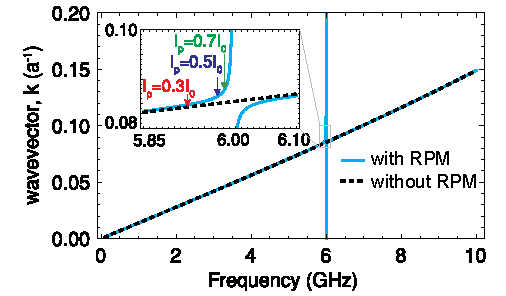
\includegraphics[width = 3.38in]{twpa_theory/disp_rpm}
\end{center}
\caption[JTWPA dispersion relation with and without RPM]{Plot of the exact JTWPA dispersion relation for $C_j$=329 fF, $L$=100 pH, $C$=39 fF, $C_c$=10 fF, $C_r$=7.036 pF, $L_r$=100 pH, and $I_0$=3.29 $\mathrm{\mu A}$.  The dispersion relation without RPM loading resonators is plotted as a dashed line and is approximately linear, though a slight curvature can be seen above 8 GHz.  The effect of the RPM loading resonators is plotted in cyan; in a very narrow band around the resonance frequency at 6 GHz, the dispersion relation diverges.  This is more clearly seen in the inset plot.  The colored labels and arrows indicate the pump frequency at which the power-dependent phase shift (proportional to $\kappa \propto (I_p/I_0)^2$) is perfectly compensated, enabling perfect phase matching.  Adapted from reference \cite{OBrien2014}.}
\label{fig:disp_rpm}
\end{figure*}

We can make the small-angle approximation in $ka$ to reduce the complexity of the problem somewhat.  This is a reasonable approximation to provide a more intuitive expression, as we expect to need a very small fractional shift in the wavevector to compensate the power-dependent phase shift.  We approximate the dispersion relation to second order in $ka$ as $2 \cos(ka) \approx 2 - (ka)^2$.  Additionally, we can assume that the junction plasma frequency $\omega_J$ is large compared to $\omega$.  This eliminates the first term in the denominator of (\ref{eq:fulldisp}).  Rearranging some terms, this gives a form in which it is easier to identify the effect of the resonator:
\begin{equation}
(ka)^2 \approx \frac{\omega^2}{\omega_0^2} + \frac{\omega^2 L C_c (1 - \omega^2 L_r C_r)}{1 - \omega^2 L_r (C_r + C_c)}
\label{eq:approxdisp}
\end{equation}
The first term is the linear dispersion of the unloaded transmission line, while the second term is the loading effect of the resonator.  We identify the loaded frequency of the resonator as the center frequency of the dispersion feature at $\omega_r = 1 / \sqrt{L_r (C_r + C_c)}$ where the denominator in the second term goes to zero.  Note that for frequencies slightly below $\omega_r$, the second term is positive, and we have achieved the desired local shift in the wavevector needed to achieve phase matching.  We have named this new phase matching technique ``resonant phase matching'' (RPM).  A plot of the resulting dispersion relation is shown in Figure \ref{fig:disp_rpm}, demonstrating the creation of the stop band and showing the divergence of the dispersion relation near $\omega_r$.



\section{Amplifier performance with resonant phase matching}\label{s:rpm_perf}

\subsection{Gain and bandwidth}

\begin{figure}
\begin{center}
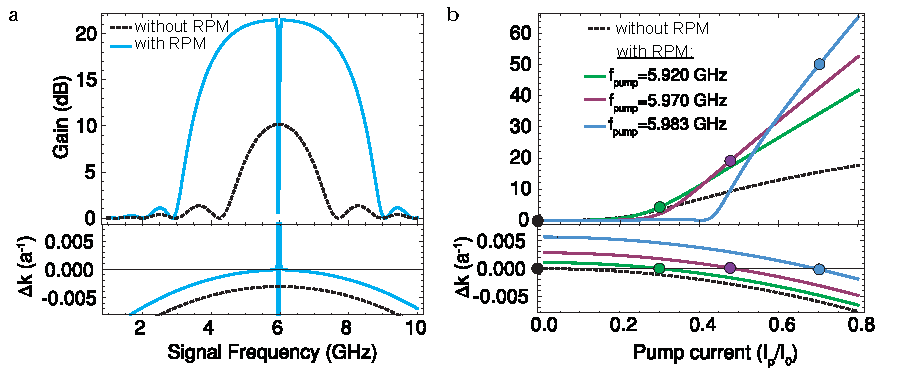
\includegraphics[width = 6in]{twpa_theory/twpa_gain}
\end{center}
\caption[JTWPA gain and phase mismatch]{Gain of a 2000 unit cell JTWPA with and without RPM loading structures. \textbf{a} The gain as a function of signal frequency in dB with RPM (cyan) and without (black dashed) for a pump current of 0.5$I_0$ and a pump frequency of 5.97 GHz.  The plot below shows the phase mismatch with RPM (cyan) and without (black dashed).  The device with RPM is perfectly phase matched at zero detuning, and becomes poorly phase matched due to the curvature of the dispersion relation as the detuning is increased.  \textbf{b} The peak gain as a function of pump current without RPM (black dashed) and with RPM for three different pump frequencies, which phase match the parametric amplification process for pump currents of 0.3 $I_0$ (green), 0.5 $I_0$ (purple), and 0.7 $I_0$ (cyan). The plot below shows the phase mismatch as a function of pump current. The dots mark the pump current where perfect phase matching is achieved.  Adapted from reference \cite{OBrien2014}.}
\label{fig:twpa_gain}
\end{figure}

Now that we have created a dispersion relation that exactly satisfies (\ref{eq:deltak}), we expect to achieve gain which grows exponentially in the length of the device.  To understand the frequency dependence of the gain, we need to examine the exact form of the exponential gain coefficient (\ref{eq:g}).  From Appendix \ref{a:twpa_paramp}, the frequency and wavevector dependence of the coupling coefficients $\kappa_s$ and $\kappa_i$ are
\begin{align}
\kappa_s &\propto \frac{(2 k_p - k_i) k_s k_i}{\omega_s^2} \\
\kappa_i &\propto \frac{(2 k_p - k_s) k_s k_i}{\omega_i^2}.
\end{align}
Re-expressing $\omega_s = \omega_p + \Delta$, $\omega_i = \omega_p - \Delta$, and assuming for the moment an approximately linear dispersion relation $k \propto \omega$, we can write the frequency dependence of $g$ for $\Delta k = 0$ as
\begin{equation}
g \propto \sqrt{\omega_p^2 - \Delta^2}.
\label{eq:g_vs_f}
\end{equation}
Thus, even for perfect phase matching, we expect the gain to decrease as the pump-signal detuning increases.  Due to the finite curvature of the dispersion relation, the phase matching will also only be close to perfect at small detuning, so this will also contribute to setting the bandwidth of the amplifier.

In Figure \ref{fig:twpa_gain}a, we show the gain and phase mismatch for a 2000 unit cell device with pump current $I_p = 0.5 I_0$ at $f_p = 5.97$ GHz and the same device parameters listed in Figure \ref{fig:disp_rpm}.  For perfect phase matching, we predict a gain of just over 20 dB with a very large bandwidth, nearly an entire octave centered at 6 GHz.  Without the phase matching improvement from RPM, the gain is only 10 dB with a bandwidth of a bit under 2 GHz.  The bandwidth is set by a combination of the phase mismatch due to the band curvature and the detuning dependence (\ref{eq:g_vs_f}).  The effect of RPM can be understood well by the bottom plot in \ref{fig:twpa_gain}b; for low pump powers, the phase mismatch is positive, and decreases to cross zero.  In the vicinity of the zero crossing, the four-wave mixing process is efficient and the gain increases exponentially in the pump current.

\begin{figure}
\begin{center}
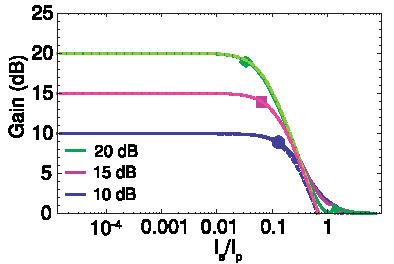
\includegraphics[width = 2.63in]{twpa_theory/twpa_comp}
\end{center}
\caption[JTWPA gain compression]{Amplifier gain as a function of input signal current, normalized to the pump current, for a small signal gain of 10, 15, and 20 dB obtained with a pump current of $0.5 I_0$ and device lengths of 1150, 1530, and 1900 unit cells. The approximation for the gain depletion (dashed lines) from (\ref{eq:gen_comp}) is in excellent agreement with the result obtained by solving the full nonlinear dynamics (solid lines).   Adapted from reference \cite{OBrien2014}.}
\label{fig:twpa_comp}
\end{figure}

\subsection{Dynamic range}

The upper limit of the dynamic range of a parametric amplifier is given by pump depletion: the pump transfers energy to the signal and idler which reduces the parametric gain. To investigate this regime, we solve for the coupled wave equations without the undepleted pump approximation. This derivation appears as Appendix 4 in reference \cite{OBrien2014}, and the resulting curves are plotted as solid lines in Figure \ref{fig:twpa_comp}. The gain as a function of input signal power calculated from the full analytical expression is in excellent agreement with the approximate, general solution for pump depletion in a four-wave parametric amplifier \cite{kylemark_semi-analytic_2006}:
\begin{equation}
G=\frac{G_0}{1+2 G_0 I_{s}^2/I_{p}^2} \label{eq:gen_comp}
\end{equation}
where $G_0$ is the small signal power gain in linear units and $I_{s}$ and $I_{p}$ are the input signal and pump currents. From (\ref{eq:gen_comp}), the gain compression point is approximately $P_{1 \rm dB}=P_{p}/(2 G_0)$. Thus, the threshold for gain saturation is independent of the specific device configuration and depends only on the small signal gain and the pump power. For the device parameters listed previously, the gain as a function of input signal current is plotted for three values of the small signal gain in Figure \ref{fig:twpa_comp}. The signal current at which the gain drops by 1 dB is marked. For a pump current of $0.5 I_0$, the signal power where the gain decreases by 1 dB is $-87$, $-93$, and $-98$ dBm for a small signal gain of 10, 15, and 20 dB, respectively. These gain compression points are consistent with the approximate relation with the pump power of -69 dBm.  A 1 dB input compression power of -98 dB is about 12 dB higher than achieved by any JPA with comparable gain.

\subsection{Parameter regime}\label{s:twpa_param}

The parameters chosen for these theory plots are the result of extensive engineering using the full theory of the device.  Simplifying the expression for the gain by assuming perfect phase matching and neglecting the effects of the resonant element and the junction resonance on the dispersion, we find that the exponential gain coefficient is directly proportional to the wave vector $g\propto k_p I_p^2/I_0^2$. Thus, for a fixed pump strength relative to the junction critical current, the gain coefficient is proportional to the electrical length. In other words, a larger wave vector and thus a slower effective wave propagation velocity leads to a larger effective nonlinearity due to the higher energy density; this effect is well known in photonic crystals \cite{soljacic_photonic-crystal_2002}. Because the characteristic impedance is designed to be $Z \approx \sqrt{L/(C+C_c)} \approx 50$ $\Omega$, the ratio of the inductance and capacitance is fixed. The wave vector is proportional to the product of the capacitance and inductance $k \approx (\omega/a) \sqrt{L(C+C_c)}$.

Increasing both the capacitance and inductance or decreasing the unit cell size are effective strategies for increasing the gain per unit length while maintaining impedance matching for 50 $\Omega$ feedlines.  However, because the junction critical current $I_0$ (and the resulting maximum pump power) scales inversely with the inductance \eqref{eq:LJ}, increasing the wavevector to increase the gain also decreases the dynamic range of the amplifier.  Additionally, the minimum size of the unit cell is constrained due to the finite physical extent of the capacitors and inductors. The parameters in the design discussed here sit in a surprisingly small area of the total parameter space where we realize an amplifier that simultaneously achieves large gain, large bandwidth, and large dynamic range.

Although the very large gain operation shown in the top panel of \ref{fig:twpa_gain}b is impressive at first glance, operation with such large gain is unrealistic due to several physical constraints.  First, the total power in a pump wave with $I_p = I_0 \sim 5$ $\mu$A is $P_p \sim -62$ dBm.  Enforcing our general constraint on power scales for linear operation of a parametric amplifier from section \ref{s:jpa_perf} and formalized in (\ref{eq:gen_comp}), our amplified output signal power should be no larger than $P_p - 20$ dB.  Without any signal at the input, the amplifier must still amplify any input noise present, which corresponds to at least $\hbar \omega$ per mode of quantum fluctuations across the entire bandwidth of the device \eqref{eq:half_quantum}.  This results in an input noise power roughly given by $P_Q \approx \hbar \omega B = -108$ dBm for $B = 4$ GHz centered at $\omega/2 \pi = 6$ GHz.  In order to satisfy $P_Q + G < P_p - 20$ dB, the gain must be no larger than about 26 dB for the input noise power to not drive the amplifier into gain compression.  This constraint could be relaxed by reducing the bandwidth, but gain exceeding 20 dB is not normally necessary to achieve quantum-limited operation for the whole measurement system.

A further constraint comes from the fact that we have so far ignored the possible effect of multiple reflections at the input and output of the amplifier.  In any real device, the matching between the nonlinear transmission line and the linear input and output feedlines will be imperfect, so some fraction of the amplified signal will be reflected from the output back to the input.  If the reflection coefficient is $R$ in dB, then a signal at the input amplified by the gain $G$ reflects back from the output at the level of $G+R$ and is reflected at the input back into the amplifier again at $G+2R$.  For the amplifier to be stable, this feedback gain must be less than 0 dB; realistically, we would like it to be much smaller than 0, otherwise we will set up a large standing wave inside the amplifier which will produce large ripples in the gain profile at harmonics of twice the frequency corresponding to the electrical length of the JTWPA.  For typical microwave devices, $R = -20$ dB is considered to be well-matched, and reducing this further is quite challenging especially in a broadband circuit.  Thus, if $G$ is larger than 40 dB, the amplifier will be unstable; moreover, if we want the total reflection $G+2R$ to be -20 dB or better, $G \lesssim 20$ dB.

\subsection{Effect of finite losses}\label{s:twpa_loss_theory}

Although superconducting circuits are generally low-loss, there will still be some attenuation at microwave frequencies due to effects such as dielectric loss.  To describe the attenuation of propagating waves in the transmission line, we use a complex wavevector, $k=k'+i k''$, where the real ($k'$) and imaginary ($k''$) components describe phase evolution and attenuation, respectively, as a function of position. Including material damping, the differential equation for the signal and idler amplitudes in a rotating frame is $\mathbf{u}'(x)=\mathbf{M}(x) \mathbf{u}(x)$ where $\mathbf{u}=[a_s  ~ a_i]^T$ and 
\begin{align}
\mathbf{M}_f = 
\begin{bmatrix}
- i\frac{\Delta k}{2}-k''_s & i\kappa_s \\
-i\kappa^*_i            & i\frac{\Delta k}{2}-k''_i
\end{bmatrix} \label{eq:signallossy}
\end{align} 
where $\Delta k=2k_p-k_i-k_s+2\alpha_p-\alpha_s-\alpha_i$ is the phase mismatch, $k_{p,s,i}$ are the wavevectors in the weak field limit, $\kappa_{s,i}$ are the coupling constants for the signal and idler, $\alpha_{p,s,i}$ describe the nonlinear phase shifts (defined in Appendix \ref{a:twpa_paramp}), and $k''_{s,i}$ are the imaginary components of the signal and idler wavevectors. In a lossy nonlinear transmission line, the pump amplitude decays with position leading to position dependent phase mismatch and coupling constants; however, if the attenuation is small, the effect of pump attenuation can be approximated by a position independent phase mismatch and coupling constant with a reduced pump amplitude $A'_p=A_p\exp({-k''_p L/2})$. The solution to these coupled differential equations is then $\mathbf{u}(x)=e^{\mathbf{M}x} \mathbf{u}(0)$. The signal amplitude in the lab frame is $a_s(x)=[1,0]\mathbf{u}(x)[1,0]^T e^{i(\Delta k/2 + \alpha_s)x}$ with gain $G=|a_s(L)/a_s(0)|^2$. 

\subsection{Quantum efficiency with distributed loss}\label{s:twpa_dist_loss}

Because the loss in the JTWPA is distributed along the amplifier, losses further down the device should participate less strongly in setting the quantum efficiency than losses near the beginning.  This follows from the same intuition that losses following a high-gain amplifier should not participate strongly in setting the noise temperature of the system as long as the gain is significantly larger than the loss.  To account for the reduction in quantum efficiency attributable to distributed loss in the amplifier, we model the JTWPA as a series of cascaded ideal phase-preserving amplifiers and lumped attenuation elements, shown schematically in Fig. \ref{fig:chained_caves_amp}.

\begin{figure*}
\begin{center}
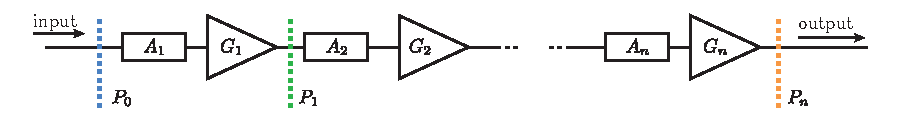
\includegraphics[width=6in]{twpa_theory/chained_caves_amp}
\end{center}
\caption[Distributed amplifier loss model]{Block diagram of the model for distributed loss and gain, showing a series of discrete attenuators $A_i$ each followed by a ideal phase-preserving amplifier with gain $G_i$.}
\label{fig:chained_caves_amp}
\end{figure*}

At the input to the amplifier at plane $P_0$ (blue dashed line) we have input noise $N_0 = N_Q = 1/2$, in units of quanta.  To calculate the noise at plane $P_1$ (green dashed line) following the lumped attenuation $A_1$ and gain element $G_1$ (both given in linear power units), we must take into account the additional quantum fluctuations added by the attenuation, $N_{\textrm{atten}} = N_Q(1-A_1)$, and the ideal phase-preserving amplifier
\begin{equation}
N_{\textrm{amp}} = N_Q(1-1/G_1)
\label{eq:caves_noise}
\end{equation}
(referred to the amplifier's input) \cite{Caves1982a}.  The total noise at plane $P_1$ is thus $N_1 = G_1 ( N_0 A_1 + N_Q (1 - A_1) + N_Q(1 - 1/G_1))$ \footnote{Our choice of ordering of the attenuation element and the gain element is arbitrary, though placing the attenuation block first gives a lower bound on $\eta$ rather than an upper bound.  For many hundreds of elements, the noise calculated for both orderings converge.}.  We can generalize this into a recurrence relation
\begin{equation}
N_i = N_{i-1}A_i G_i + N_Q (1 - A_i) G_i + N_Q (G_i - 1)
\label{eq:caves_recurr}
\end{equation}
which can be summed numerically for any distribution of $A_i$ and $G_i$ to find the total noise at the output $N_n$.  Referring the noise back to the input of the amplifier by dividing by the total transmission $T = \prod_{i=1}^n A_i G_i$ allows the expected quantum efficiency to be calculated as
\begin{equation}
\eta = (N_n / T)^{-1}
\label{eq:eta_D}
\end{equation}
assuming that the total amplifier gain is large enough to saturate (\ref{eq:caves_noise}) in the absence of loss.









\chapter{JTWPA characterization}
\label{c:twpa_exp}

The experimental results presented in this chapter correspond to the sixth JTWPA design revision.  For reasons that remain largely unknown, the first few generations of devices suffered from large insertion losses that prevented the demonstration of compelling amplifier performance.  Some of these results appear in reference \cite{slichterthesis}.  The fourth through sixth design revisions were fabricated at MIT-Lincoln Labs (LL), and resulted in generally better device performance.  These devices were primarily designed at QNL, though the professional mask layout team at LL did much of the layout in generations five and six using automated scripts, permitting mask design revisions to be made much more easily.  The sixth generation design revision was the first to incorporate RPM loading structures, in concert with the development of the dispersion engineering theory in 2014.  Many, many measurements were conducted over the entire course of the development of the JTWPA; from measurement records, the experiments on generations four, five, and six comprised seven, 23, and 30 dilution refrigerator cycles, respectively, in the period from August 28, 2012 through the final cooldown for generation six on January 1, 2015.

\section{Device fabrication}\label{s:twpa_fab}

\begin{figure*}
\begin{center}
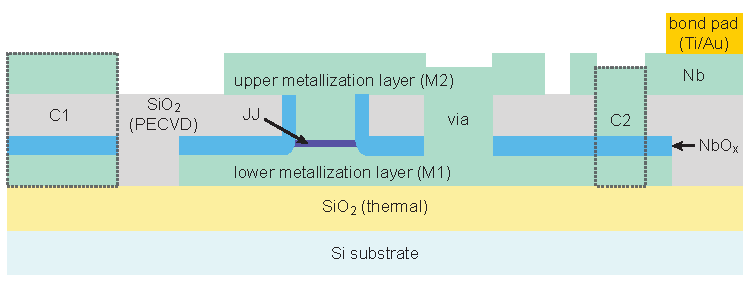
\includegraphics[width=5in]{twpa_exp/DSM_stackup.pdf}
\end{center}
\caption[Deep submicron process layers]{Schematic of the DSM process layers.  Metal layers are 150 nm thick, the PECVD layer is 200 nm thick, and the NbO$_x$ layer is 50 nm thick.  Schematic is not shown to scale.}
\label{fig:DSM_stackup}
\end{figure*}

The RPM-JTWPA is a fairly complex device, requiring the precision fabrication of five lumped-element components per unit cell of the device, and about 2000 unit cells are required to achieve enough gain to approach quantum-limited system noise.  For high-quality amplifier operation, these components should have a high degree of uniformity, requiring tight controls and process tests.  The foundry at LL is quite sophisticated, with extensive process controls including a test suite of co-fabricated structures to characterize the process performance across an entire 200 mm wafer.  The JTWPA is fabricated in the deep submicron (DSM) process, primarily used for manufacturing rapid single flux quantum (RSFQ) superconducting digital electronics, with many thousands of junctions per chip.  For a very complete description of this process, see reference \cite{Tolpygo2014}.  A schematic of the metalization and dielectric layers in DSM is shown in Fig. \ref{fig:DSM_stackup}. DSM is a fully planarized Nb/Al-AlOx/Nb trilayer process fabricated on 200 mm wafers using a modern, CMOS compatible toolset. Process modules include 248 nm photolithography, anodization, high-density plasma etching, PVD metal deposition, PECVD SiOx deposition, and chemical mechanical polishing.

Devices are fabricated on a 750 $\mu$m silicon substrate (pale blue) with a 500 nm layer of thermal SiO$_2$ (pale yellow).  Josephson junctions are defined using 248 nm optical lithography (stepper, 5x reduction) and subtractive dry etching of the Nb/Al-AlOx/Nb trilayer; the Al-AlOx is shown as a thin dark purple stripe.    Anodization of the lower Nb layer forms a thin NbO$_x$ protective layer around the junction (blue).  The inter-layer dielectric is a low-temperature PECVD silicon oxide (light gray).  The lower and upper Nb wiring layers are shown in pale green (M1 and M2, respectively); electrical connections between the layers are formed using vias (center-right).   Parallel-plate capacitors are formed implicitly where the upper and lower metallization layers overlap due to the intermediate PECVD and NbO$_x$ layers (C1, shown at left and outlined in a dashed line).  An additional high-capacitance structure can be formed by creating a via from the upper metallization layer to the anodization layer (C2, shown at right and outlined in a dashed line); C2 provides a specific capacitance approximately 35 times larger than C1.  Electrical contact is made to the chip through titanium/gold bond pads (yellow).

\begin{figure*}
\begin{center}
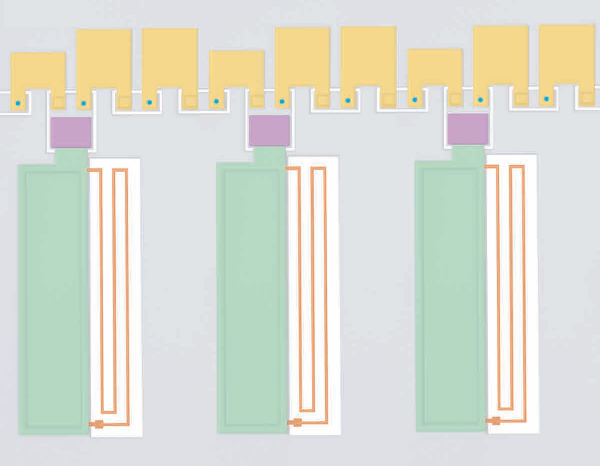
\includegraphics[width=4in]{twpa_exp/chip_false_color.pdf}
\end{center}
\caption[RPM JTWPA false-color optical micrograph]{False-color optical micrograph of chip layout.  M1 is shown as gray, with cutouts to form islands and accommodate the meander inductor.  JJs are drawn in light blue.  The top plate of the capacitance to ground is formed from M2 and colored yellow.  The coupling capacitance to the resonator is formed from C1; the top plate (M2 layer) is colored purple.  The resonator capacitance is formed from C2; the top plate (M2 layer) is colored green.  The resonator meander inductor is colored orange; the via from M2 to M1 is the wider square at the bottom of the trace.  The spacing between Josephson junctions is 16 $\mu$m.}
\label{fig:chip}
\end{figure*}

A false-color optical micrograph of about 10 unit cells is shown in Fig. \ref{fig:chip}.  The ground plane of the JTWPA is formed from M1.  The primary trace forming the transmission line itself is formed from M2, utilizing C1 for capacitance to ground.  A small ground plane cutout surrounds an M1 island, accommodating the Josephson junction and a via back up to M2.  The dispersion-modifying resonators are capacitively coupled to this island through C1.  A meander inductor is formed from M2 inside a ground plane cutout and is electrically connected to ground at the end with a via.  The capacitance for the resonator is formed from C2.

\begin{figure*}
\begin{center}
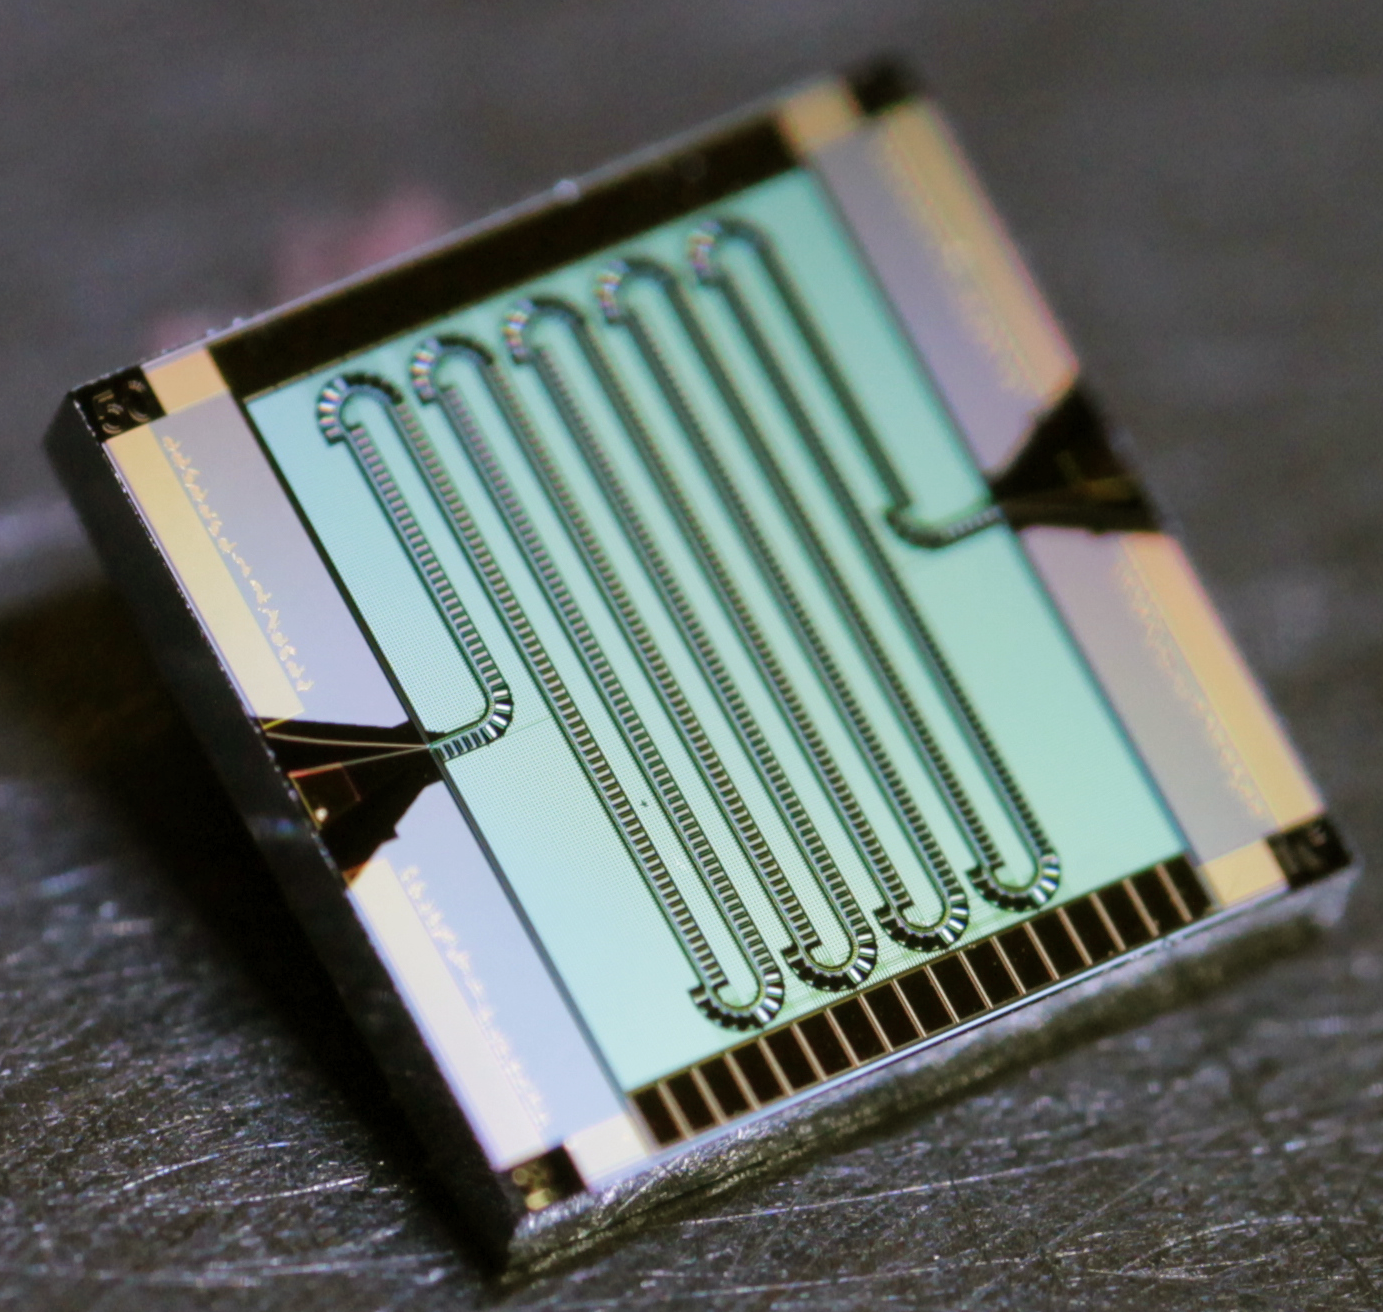
\includegraphics[width=4.6in]{twpa_exp/chip_pic.png}
\end{center}
\caption[RPM JTWPA chip photograph]{Macro photograph of a 2037 JJ RPM JTWPA.  The chip is 5 mm $\times$ 5 mm.}
\label{fig:chip_pic}
\end{figure*}

We use process monitor structures distributed across the 200 mm wafer to determine the junction critical current density $J_c = 5.8$ $\mu$A/$\mu$m$^2$ and junction specific capacitance $C_s = 70$ fF/$\mu$m$^2$.  The particular JTWPA device which is the main subject of this chapter features 1 $\mu$m diameter junctions with critical current $I_0 = 4.6$ $\mu$A, intrinsic junction capacitance $C_J = 55$ fF, and an external capacitance to ground $C = 45$ fF shunting the junction.  The critical current density was somewhat higher than designed, resulting in a small-signal impedance of 40 $\Omega$. When the JTWPA is pumped, the effective Josephson inductance increases, resulting in a small increase in impedance of approximately 2 $\Omega$. A better match to 50 $\Omega$ has been measured in similar devices with critical current densities closer to the target parameters.  A photograph of a 2037 junction device is shown in Figure \ref{fig:chip_pic}.

\begin{figure*}
\begin{center}
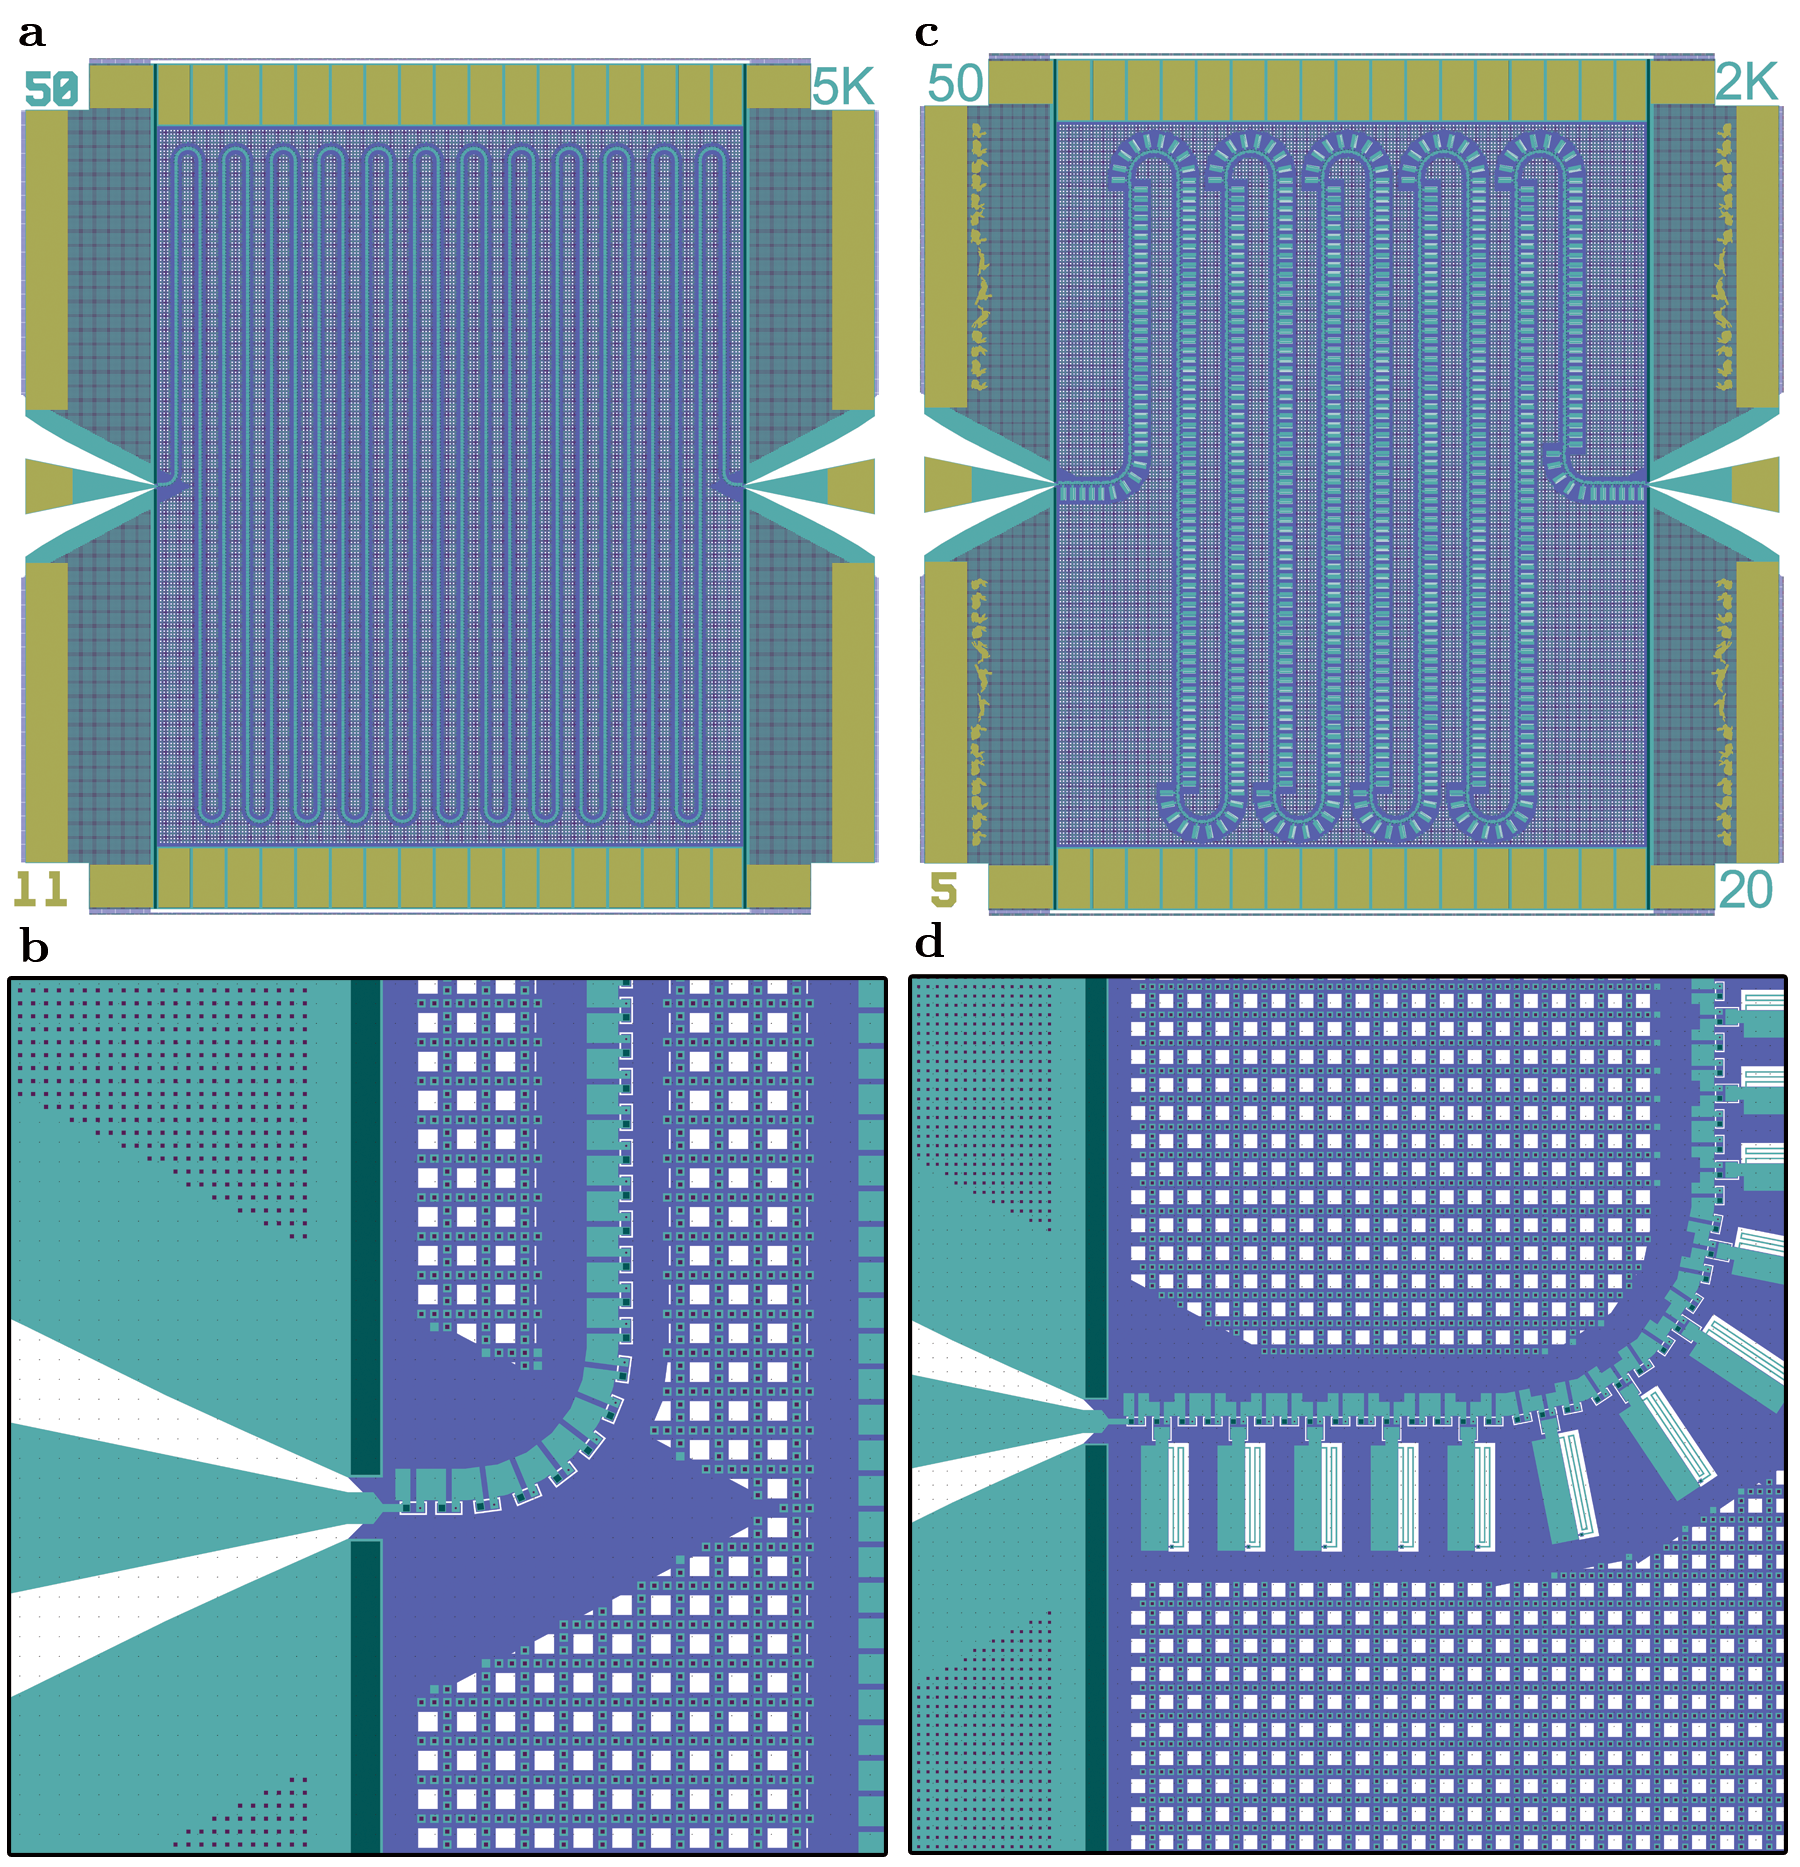
\includegraphics[width=6in]{twpa_exp/masks.png}
\end{center}
\caption[Example JTWPA layout masks]{\textbf{a} Chip layout for 50 $\Omega$ 5022 JJ non-RPM device, from Reticle A. \textbf{b} Close-up of \textbf{a}, showing CPW-to-microstrip transition and nonlinear transmission line segment. \textbf{c} Chip layout for 50 $\Omega$, 2037 JJ RPM device with 20 fF coupling capacitors, from Reticle B. \textbf{d} Close-up of \textbf{c}.}
\label{fig:masks}
\end{figure*}

Several other device designs were co-fabricated along with the particular chip design which is the subject of the bulk of the results in this chapter.  All in all, two full reticles were used for generation six, providing 13 individual chip designs in each reticle with 3 chips of process test structures.  Reticle A was dedicated to JTWPAs without RPM resonators, as these devices were known to work well.  Reticle B was dedicated to JTWPAs with the very first attempt at RPM loading, which turned out to work quite well and produce the first JTWPAs with significant gain and nearly quantum-limited noise.  Various images of the mask layouts from generation six are shown in Figure \ref{fig:masks}.

\subsection{Loss tangent extraction}

\begin{figure*}
\begin{center}
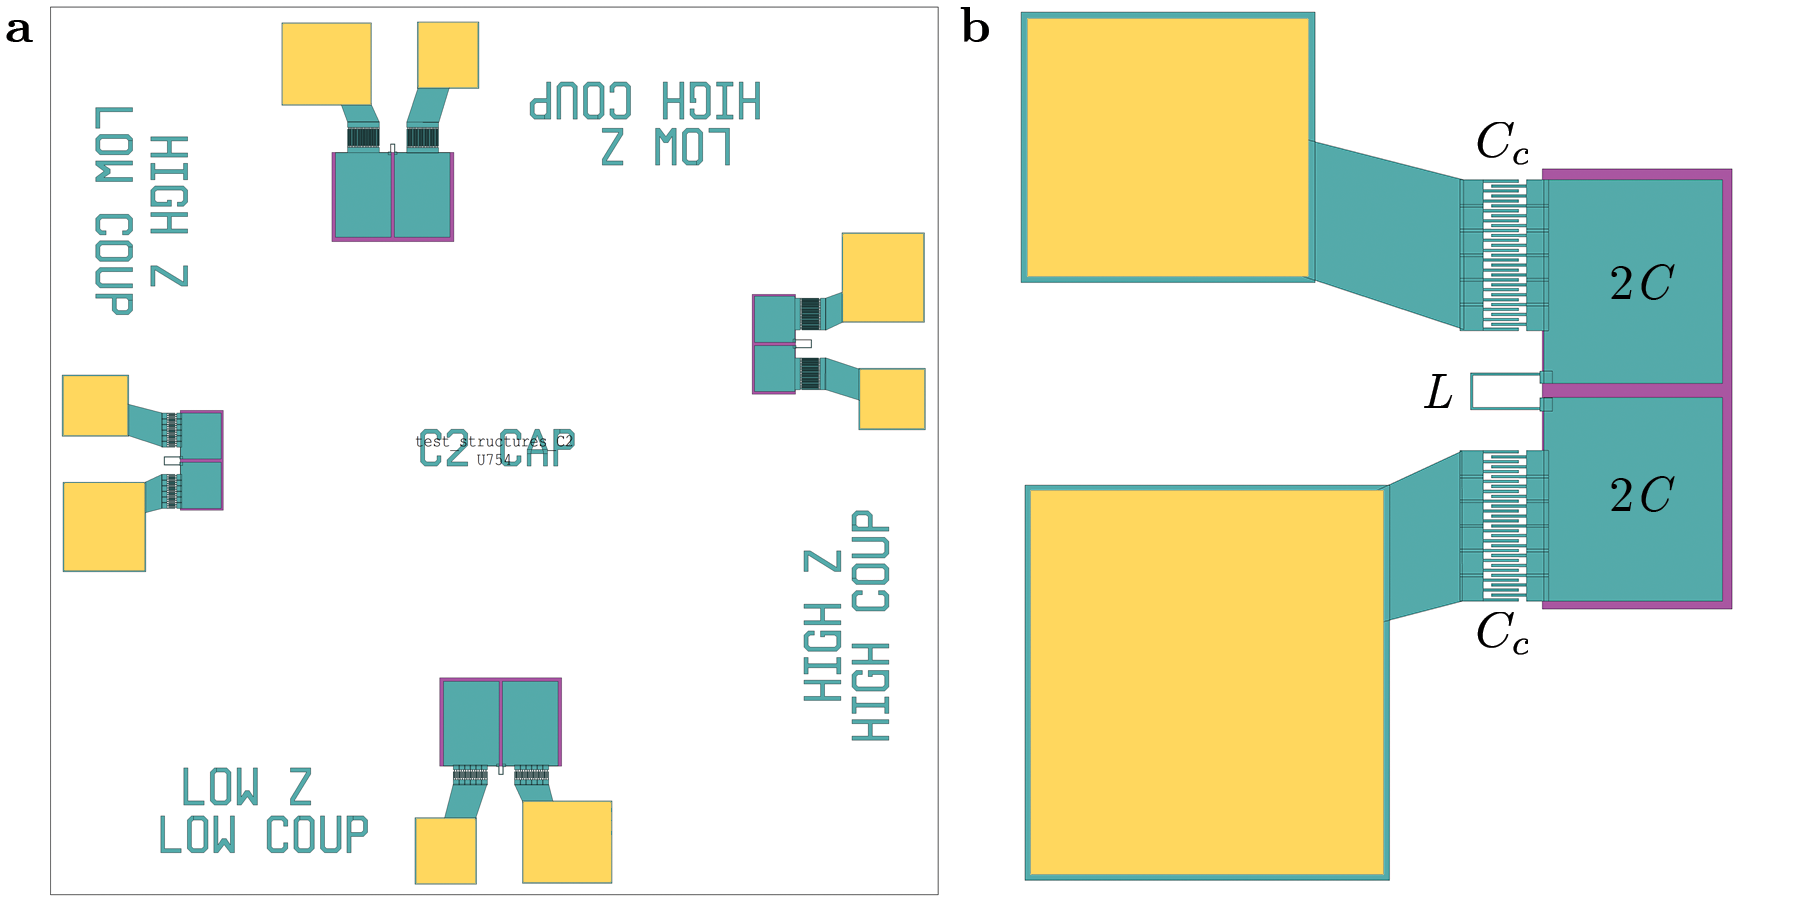
\includegraphics[width=6in]{twpa_exp/test_res.png}
\end{center}
\caption[Test resonator masks]{\textbf{a} Chip layout for C2 layer test resonators.  \textbf{b} Close-up of the low-coupling, high-impedance test resonator from the left side of \textbf{a}.}
\label{fig:test_res}
\end{figure*}

The loss tangents of the C1 and C2 capacitors were determined by measuring the internal quality factor of lumped-element test resonators.  The chip layout for the C2 capacitor test resonators is shown in Figure \ref{fig:test_res}a.  The equivalent structures for measuring the C1 layer are similar, though the capacitors have a much smaller footprint due to the larger specific capacitance.  The resonators are a differential design but are normally measured in a CPW launch with one side of the resonator wirebonded to ground.  Due to the differential design, the two capacitors which form $C$ combine in series, thus the total capacitance is half that of each physical capacitor.  The resonators are all targeted at the same nominal frequency, but with two impedance variations and two coupling strength variations.

The total inductance $L$ of the structure is purely geometric, and can be accurately predicted using finite-element simulation tools.  The coupling capacitance $C_c$ is designed to be very small compared to the resonator inductance $C$ so as to avoid loading the resonant frequency.  Furthermore, $C_c$ is designed as an interdigital capacitor, which generally has a much higher intrinsic quality factor than the overlap capacitors formed by C1 and C2, and thus should not effect the total coupling strength.  Therefore, measuring the resonant frequency of the test resonators calibrates the specific capacitance for the capacitor layer under consideration, while extracting the internal quality factor $Q_i$ provides the loss tangent of the capacitor layer.  For details on the algorithm used to extract $Q_i$ from a reflection measurement, see Appendix D of reference \cite{Weber2014a}.

\begin{figure*}
\begin{center}
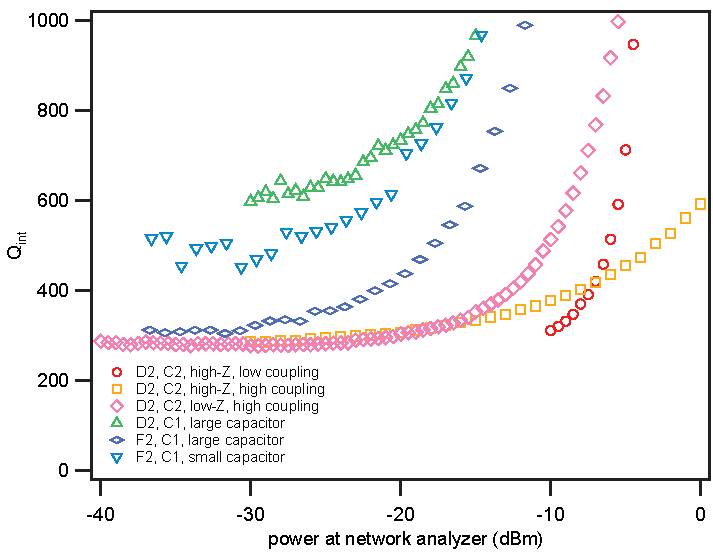
\includegraphics[width=4.75in]{twpa_exp/Qint}
\end{center}
\caption[Test resonator quality factor measurements]{Measured internal quality factors for six test resonators, three from the C1 layer and three from C2.  The traces have been offset on the power axis for clarity, to show the saturation in roughly the same regime.}
\label{fig:Qint}
\end{figure*}

If we assume that all of the internal loss in the resonator can be attributed to the dielectric loss in the capacitor, then the loss tangent of the material is just given by the inverse of $Q_i$.  The loss tangent of these types of deposited dielectrics tends to be relatively high, on the order of $10^{-3}$ to $10^{-2}$, while inductive losses and losses in the coupling capacitors should be very small compared to this.  As shown in Figure \ref{fig:Qint}, the C2 resonators have a fairly consistent $Q$ of about 300, while there is somewhat more scatter in C1 from 300 to 600 or so.  Because the transmission line capacitance is formed from C2, this is the most important loss in the system, corresponding to a loss tangent of about $3.3 \times 10^{-3}$.  Assuming no other losses in the line, the attenuation constant $\alpha$ of the transmission line in the small signal regime is then given by
\begin{equation}
\alpha = 8.686 \times \tan(\delta) \frac{\omega C Z_0}{2} = 2.03 \times 10^{-4} \frac{\mathrm{dB}}{\textrm{unit cell} \cdot \rm GHz}
\end{equation}
for $C = 45$ fF \cite{pozar1997microwave}.  Thus, a 2000 cell JTWPA should have a loss of about 1.6 dB at 4 GHz, and 4 dB at 10 GHz.

\section{Transmission measurements}

Because the JTWPA is a 2-port device and operates in a transmission mode, measuring the transmission through the device in a well-matched 50 $\Omega$ environment is the most fundamental and important measurement of device performance.  Measurements of reflection parameters are also of interest, though making this type of measurement in a well-calibrated manner in a cryogenic system is quite non-trivial and requires cryogenic calibration standards to make a meaningful measurement.  As such, I will focus on transmission measurements only.

\begin{figure*}
\begin{center}
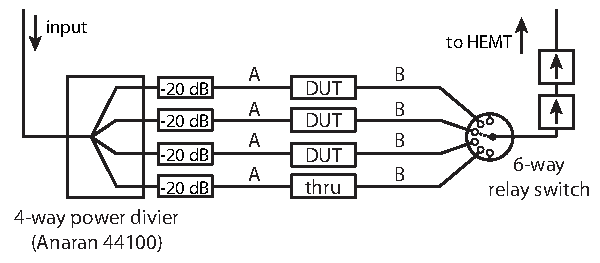
\includegraphics[width=4in]{twpa_exp/trans_meas}
\end{center}
\caption[Cryogenic calibrated transmission measurement setup]{Microwave circuit schematic for cryogenic calibrated transmission measurements, using passive input multiplexing and active output multiplexing.  Higher temperature stages not shown.}
\label{fig:trans_meas}
\end{figure*}

The cryogenic setup used for the majority of JTWPA measurements is shown schematically in Figure \ref{fig:trans_meas}.  The probe signals arrive at the cold stage of the dilution refrigerator and are passively split using a commercial 4-way 2-18 GHz power divider.  The relative power in each output is balanced to better than 0.1 dB.  A 20 dB attenuator is connected to the output of each port, ensuring the input to the device under test (DUT) is a well-matched 50 $\Omega$, and adding an effective 40 dB of isolation between each measurement arm.  With the 20 dB isolation of the splitter itself, this setup provides about 60 dB of total isolation between the measurement arms.  The output of each measurement arm is connected to one port of a 6-way microwave relay switch, which directs one of the outputs through two isolators to the HEMT amplifier, while presenting an open circuit to the other ports.  Two more DUTs could be added to this setup if the 4-way power divider is replaced by another 6-way relay switch, which was not available in the dilution refrigerator in which these experiments were conducted.

One of the splitter outputs is connected to a SMA female-female union in place of a DUT to represent the baseline calibration for the transmission measurement.  The cables used to connect the thru calibration and the DUTs to the power divider and the output multiplexing switch are nominally identical commercial flex cables made by Mini-Circuits, of lengths labeled A and B.  On one cooldown, one of the DUTs was replaced with another thru connector to check the balance of the different transmission arms; transmission through the two thru connections was indistinguishable at the 0.1 dB level.  The DUTs are normally housed in an aluminum enclosure with small slots through which SMA cables enter and leave.  The aluminum enclosure is contained within a single layer of Cryoperm magnetic shielding.  The DUTs are bolted to a copper plate which is thermalized to the cold stage of the dilution refrigerator using a thick copper wire protruding through the lid of the aluminum enclosure.  This enclosure is primarily a legacy from past experiments; because the JTWPAs are fabricated from Niobium, they become superconducting at around 9 K, much earlier in the cooldown process than when the aluminum enclosure becomes superconducting at about 1 K.  Because the JTWPA design does not involve any SQUID loops, the device behavior is not particularly sensitive to magnetic field fluctuations and so a high degree of magnetic shielding is not necessary.

\subsection{Length scaling of non-RPM devices}

\begin{figure*}
\begin{center}
\includegraphics[width=6in]{twpa_exp/trad_dat}
\end{center}
\caption[Insertion loss and gain of non-RPM JTWPAs]{\textbf{a} Insertion loss for 1k, 3k, and 5k JJ devices, with theory predictions for a capacitor quality factor $Q_i = 291$.  \textbf{b} Measured gain profiles of 1k, 3k, and 5k JJ devices at identical pumping conditions ($\sim 0.75 I_0$), after subtracting the insertion loss measured in \textbf{a}, with theory overlays for the simple theory without loss.}
\label{fig:trad_dat}
\end{figure*}

To verify the theoretical prediction of quadratic scaling with device length for JTWPAs with no explicit modification to the dispersion relation, we measured three devices from Reticle A in the same cooldown, with lengths of 1k, 3k, and 5k unit cells\footnote{In reality, we measured many more of these types of devices, as they were the focus of the work before the addition of RPM loading structures.  For clarity I focus here on just three devices of the final generation.}.  The nominal device parameters are $I_0 = 3.1$ $\mu$A, $C_j = 55$ fF, and $C = 50$ fF, and the 1k, 3k, and 5k devices actually contained 1006, 3008, and 5022 junctions, respectively.

Data from these devices are shown in Figure \ref{fig:trad_dat}.  After calibrating the transmission using the thru, we measured the insertion loss of each device.  The measured insertion loss agrees well with the losses predicted by a simple model of capacitive dielectric losses with $\tan{\delta} = 0.0034$, in good agreement with the measured loss tangent of the material.  The gain of these devices is plotted with the insertion loss subtracted, to more directly show the quadratic scaling behavior with increasing length.  The agreement between the measured gain and the theory is quite reasonable, validating the simple prediction of quadratic scaling.

\subsection{Measurements of RPM loading structures}

For the remainder of this chapter I will focus on a very complete characterization performed on a single RPM-JTWPA device.  The device parameters are those listed in section \ref{s:twpa_fab}.  I will refer to this particular amplifier as Device A.

\begin{figure*}
\begin{center}
\includegraphics[width=4.1in]{twpa_exp/twpa_trans}
\end{center}
\caption[Transmitted power and wavevector shift]{\textbf{a} Broadband small-signal power transmission, with axis scaled to clearly show the dielectric insertion loss of 1 to 4 dB.  The transmission dip associated with the RPM resonators is visible just above 7 GHz. \textbf{b} Small-signal power transmission (green) and wavevector shift (purple) in the vicinity of the dispersion feature.  The large linear component of the wavevector has been subtracted to show just the shift associated with the dispersion feature.}
\label{fig:twpa_trans}
\end{figure*}

In the small-signal regime, an RPM-JTWPA should look identical to a JTWPA without loading structures except for the presence of a large transmission dip in the vicinity of the resonant frequency of the RPM resonators.  The small-signal transmission and wavevector shift for Device A is shown in Figure \ref{fig:twpa_trans}.  The insertion loss is comparable to that measured for non-RPM devices in Figure \ref{fig:trad_dat}.  The width of the RPM stop band is significantly larger than predicted for the ideal theory; this is due to some small frequency variation in the resonators, on the order of 1\%, which is sufficient to significantly broaden the stop-band and weaken the total wavevector shift.  This frequency heterogeneity is also responsible for the large ripples in transmission and wavevector on the low-frequency side of the dispersion feature.  Although the absolute magnitude of the wavevector shift is decreased compared to theory, it is still sufficient to partially phase match the four-wave mixing process.

\subsection{Gain with RPM}\label{s:gain_with_rpm}

\begin{figure*}
\begin{center}
\includegraphics[width=4in]{twpa_exp/gain_and_dk}
\end{center}
\caption[Gain and phase mismatch comparison]{Total wavevector mismatch $\Delta k$ (left axis) and corresponding amplifier gain (right axis) for a signal at 6.584 GHz.  For the ``RPM'' traces, the pump was placed at 7.157 GHz, while the ``detuned'' traces have a pump at 6.5 GHz, far from the dispersion feature.  Theory predictions are overlaid on the data as dashed lines in complementary colors.  The total wavevector modification for the RPM case can be seen as the vertical offset on the left axis between the green and blue traces.}
\label{fig:gain_and_dk}
\end{figure*}

The effect of RPM on the device gain is shown in Figure \ref{fig:gain_and_dk}, where the wavevector mismatch and gain is plotted for a pump near the RPM feature and also for a pump far detuned.  The measured gain for the RPM case is about 10 dB larger than for the detuned case, even though the wavevector mismatch is still far from perfect at large pump powers.  The pump power axis is scaled using the sharp feature visible at the right of the plot, which roughly corresponds to the power at which the pump current exceeds the junction critical current.  This effect is used in all measurements to calibrate the pump power scale.

\begin{figure*}
\begin{center}
\includegraphics[width=6in]{twpa_exp/twpa_gain}
\end{center}
\caption[Ultra-broadband gain profile]{The gain profile measured with a pump at 7.157 GHz and a pump current of 91\% of the critical current.  A theory prediction for the measured device parameters, including the effects of loss for the signal and the pump, is overlaid as a blue dashed line.}
\label{fig:twpa_gain_exp}
\end{figure*}

The complete gain profile achieved with a pump at 7.157 GHz and $I_p / I_0 = 0.91$ is shown in Figure \ref{fig:twpa_gain_exp}.  Without exaggerating, the bandwidth achieved by Device A can be described as massive.  The gain exceeds 20 dB over a bandwidth of about 3 GHz, excluding the region near the dispersion feature, and exceeds 15 dB over an entire octave (from 4.5 to 9 GHz).  This is by far the largest bandwidth ever achieved in a Josephson parametric amplifier of any variety\footnote{This bandwidth has been superseded by a device from a subsequent seventh generation of JTWPAs, measured at LL.  That device achieved a bandwidth of 4.5 GHz with gain above 20 dB.}.  The gain profile shows a small ripple, on the order of $\pm 2$ dB, which we attribute to the impedance mismatch between the nonlinear JTWPA transmission line (which is about 42 $\Omega$ when pumped) and the linear 50 $\Omega$ feedlines to which it is coupled.  This leads to a small amount of reflection, with a period related to the electrical length of the JTWPA as discussed at the end of section \ref{s:twpa_param}.

The overlaid theory curve is based on the modified theory including the effect of finite pump and signal losses described in section \ref{s:twpa_loss_theory}.  The model parameters are determined from linear and nonlinear single-wave characterization. To obtain the wavevector, we measure the microwave transmission without a pump through the JTWPA. The real component of the wavevector is obtained from the phase of the transmitted field, $k' = (\phi(\omega)+\phi_0)/L$, and the magnitude of the transmission yields a frequency dependent imaginary wavevector, $k''=-\log(T)/(2L) \approx c_1 \omega + c_2^2 \omega^2$, where $c_1 = 2.0$ fs and $c_2 = 0.55$ fs,  away from the resonance. The signal and idler are attenuated more than the pump as the strong pump field partially saturates the frequency-dependent dielectric loss. The constant $\phi_0$ is determined from the zero-frequency limit of the wavevector. From a comparison of the experimentally-measured dispersion with the theoretical model for the wave-vector we obtain an estimate for the capacitance to ground of $C=45.6~\mathrm{fF}$. The junction parameters are obtained from electrical characterization as detailed in section \ref{s:twpa_fab}. We model the effect of inhomogeneity in the dispersion loading resonators as a single resonant mode with a loaded Q selected to best match the width of the observed transmission dip.

\section{Noise measurements}

A high-gain, broadband amplifier is only useful if the amplifier operation is quiet.  For the JTWPA, the goal is to saturate the ideal quantum lower bound on added noise, as discussed in chapter \ref{c:paramps}.  To conclusively demonstrate noise near the quantum limit, precision measurements must be made to ensure that the systematic errors are fractionally small compared to the measured value.  A noise measurement that concludes that the amplifier is quantum-limited \textit{plus or minus the quantum limit} is both uninteresting and unphysical.

\subsection{System noise temperature extraction}

The fundamental challenge for making precise cryogenic noise measurements is the need for a calibrated power reference at the cold stage of the dilution refrigerator.  Injecting a signal which is calibrated at room temperature into the system is insufficient, as the insertion loss between room temperature and the cold stage cannot be directly measured when the system is cold.  Measuring the total round-trip transmission doesn't help either, as the gain of the HEMT amplifier and the insertion loss back up to room temperature is equally unknown.  Thus, we must find some physical process which produces a calibrated reference power at the cold stage, ideally at a relevant reference plane for characterizing an amplifier.

The two most commonly-used physical processes are the Johnson noise of a variable-temperature matched load \cite{Fernandez1998} and the shot noise of a tunnel junction \cite{Spietz2003}.  Although both of these techniques provide a precisely-calibrated broadband noise level, they suffer from the same general class of drawbacks: each technique requires an intermediate microwave network between the calibrated source and the remainder of the microwave measurement chain which is unrelated to the general measurement setups in which the amplifiers will be used.  For the variable-temperature load, an intermediate piece of coaxial cable is needed to permit the temperature of the load to be varied independently of the rest of the measurement chain.  Because thermal conductivity in a metal is provided by the electrical conductivity at dilution refrigerator temperatures, this typically implies that this cable is made of a lossy material such as stainless steel, introducing an unknown insertion loss on the order of 1-2 dB.  For the shot noise tunnel junction source, a bias tee is needed to inject the DC voltage to bias the tunnel junction, introducing an unknown insertion loss on the order of 1-2 dB.  As a result of these unknown losses, the total system noise temperature reported using these techniques typically comes with systematic uncertainty of the same order, preventing a precise determination of the system noise \cite{Castellanos-Beltran2008,Mutus2014}.

\subsection{Circuit QED power calibration}

\begin{figure*}
\begin{center}
\includegraphics[width=5in]{twpa_exp/noise_schem.pdf}
\end{center}
\caption[Microwave measurement schematic for system noise measurement]{Schematic diagram of microwave measurement setup for system noise temperature measurements.  Gain measurements are made \textit{in situ} by injecting an additional measurement signal from a vector network analyzer through a directional coupler on the pump line at room temperature.}
\label{fig:noise_schem}
\end{figure*}

Instead of these calibrated noise reference techniques, we utilize the AC Stark shift of a cQED system to precisely calibrate the photon number occupation of the cavity.  A schematic of the full microwave setup used in these experiments is shown in Fig \ref{fig:noise_schem}.  By independently measuring the cavity frequency $\omega_r$ and output coupling rate $\kappa$, the output power is then precisely determined as $P = \kappa \hbar \omega_r \bar{n}$.  This is the same technique as is used to determine $\eta_\mathrm{det}$ in section \ref{s:det_meas_eta}.  Because we use a cQED system as the source of the power calibration, there is no additional uncertainty in determining the relevant system noise temperature delivered by a particular parametric amplifier in a real experimental context, as the experiment itself serves as the reference plane.  The primary downside of this technique compared to a calibrated noise reference is the fundamentally narrowband nature of the cavity power calibration, so we will only be able to extract the system noise at the cavity frequency.

The cQED system used here was again a single-junction 3D transmon.  The qubit had a transition frequency $\omega_{qb}/2 \pi = 3.58$ GHz, measured precisely with Ramsey oscillations, and $T_1 = 22$ $\mu$s.   The cavity parameters are directly measured by fitting the cavity transmission spectrum to a Lorentzian function, as shown in Figure \ref{fig:kappa}, resulting in $\omega_r / 2 \pi = 5.984$ GHz and $\kappa / 2 \pi = 18.5$ MHz.

\begin{figure*}
\begin{center}
\includegraphics[width=3.75in]{twpa_exp/kappa}
\end{center}
\caption[Lorentzian fit of cavity resonance]{Lorentzian fit to cavity resonance.  The measured cavity transmission spectrum deviates slightly from a perfect Lorentzian profile; we attribute this variation to transmission ripple in the microwave measurement chain, which is generally smooth but becomes significant on the order of 30 MHz.}
\label{fig:kappa}
\end{figure*}

We calibrate the dispersive shift $\chi$ using two techniques.  First, we utilize the same AC Stark shift and measurement dephasing technique described in section \ref{s:chi_cal}, though in this round of measurements we took a significantly larger quantity of data to reduce the noise and improve our estimate of $\chi$ to the 1\% level.  The extracted AC Stark shift and dephasing rates versus measurement power are shown in Figure \ref{fig:gamma_and_stark}a along with the resulting calibration between input power and $\bar{n}$ (Figure \ref{fig:gamma_and_stark}b); from the fits, we extract $\chi = 584 \pm 5$ kHz.

As an independent check on this result, we directly measure the phase shift in the transmitted microwave signal for different qubit states.  This data is shown in Figure \ref{fig:gamma_and_stark}c.  We use postselection to purify an ensemble of qubit states in $|0\rangle$ and $|1\rangle$ (see section \ref{s:weak_meas} for more details).  We then integrate an intermediate measurement period and plot the resulting points in the IQ plane.  We measure an angular separation $\Delta \theta = 7.3$ degrees, implying a value for the ratio $\chi / \kappa = \frac{1}{2} \tan{(\Delta \theta/2)} = 3.18 \times 10^{-2}$.  From the direct measurement of $\kappa$ and the value for $\chi$ extracted using the AC Stark shift measurement, we find $\chi / \kappa = (3.16 \pm 0.03) \times 10^{-2}$, in excellent agreement.  There is a slight 1\% asymmetry in the length of the two coherent state vectors, likely due to the measurement frequency not being exactly at the midpoint between the cavity frequencies associated with the first two qubit states.

This direct measurement of $\Delta \theta$ requires precisely calibrating the demodulation setup.  In general, the three first-order imperfections in the demodulation setup are unequal gains and DC offsets in the low-frequency signal path for the I and Q outputs, as well as skew in the axes represented by I and Q (implying some mixing of one axis into the other).  All of these effects can be measured simultaneously by injecting a signal which is slightly detuned from the local oscillator, producing oscillations in I and Q at the detuning frequency.  By fitting these oscillations to sine and cosine and extracting the offset, amplitude, and phase shift, we can calculate a transformation which removes all of these effects to first order. 

\begin{figure*}
\begin{center}
\includegraphics[width=6in]{twpa_exp/gamma_and_stark}
\end{center}
\caption[$\chi$ calibration, two ways]{\textbf{a} Linear fits to measured dephasing rate and AC Stark shift versus weak measurement power.
\textbf{b} Calculated mean cavity photon occupation from calibrated value of $\chi$ and the measured AC stark shift. \textbf{c} Purified qubit readout histograms.  We independently estimate the ratio $\chi / \kappa$ by measuring the phase shift in the transmitted microwave signal for ensembles of purified qubit states, finding a phase shift between the ground state and excited state histograms of 7.3 degrees.}
\label{fig:gamma_and_stark}
\end{figure*}

\subsection{Noise power}\label{s:noise_pow}

With the photon number calibration in hand, measuring the system noise temperature referred to the cavity output is as simple as measuring the ouput noise spectrum of the microwave measurement chain while simultaneously injecting a calibrated signal power.  In practice, we excite the cavity with a calibrated $\bar{n}$ and measure the resulting power at the output using a spectrum analyzer.  We then turn the cavity excitation off, and inject a tone directly down the JTWPA pump line, bypassing the cavity, and adjust the generator power until we measure the same power at the spectrum analyzer.  This procedure calibrates this signal power to the same plane as the photon number calibration, but avoids any extra noise associated with thermally-induced qubit transitions or small qubit-cavity nonlinearities at high drive powers from contaminating the amplifier measurement.

\begin{figure*}
\begin{center}
\includegraphics[width=4in]{twpa_exp/snr_trace}
\end{center}
\caption[Calibrated output noise spectra]{Calibrated output noise spectra.  The spectrum taken with the pump on is referred to back to the input by subtracting the measured amplifier gain.}
\label{fig:snr_trace}
\end{figure*}

Noise power spectra taken of the output microwave field in the vicinity of the cavity frequency are shown in Figure \ref{fig:snr_trace}.  The coherent tone corresponding to a mean cavity occupation $\bar{n} = 3.62 \pm 0.04$ allows us to calibrate a cavity-output-referred power axis (left) as well as a system noise temperature axis using Boltzmann's constant and the 10 kHz measurement bandwidth (right).  With the JTWPA pump off we extract a system noise of $9.01 \pm 0.23$ K.  This is a very reasonable number; the HEMT amplifier is manufactured by Low Noise Factory (model LNC4-8A) and has a specified noise temperature of 3 K.  If the HEMT is meeting this specification, then a 9 K system noise implies an insertion loss of 4.8 dB between the cavity and the HEMT, including 2.0 dB of loss in the JTWPA.  Considering the passive microwave network in this portion of the measurement chain contains a directional coupler and three isolators, an insertion loss of 2.8 dB is very reasonable (a typical rule of thumb is 0.5 to 1 dB per component).  We turn the pump on and measure a signal gain of 21.6 dB; we refer the resulting noise level to the cavity output by subtracting this gain from the measured trace, permitting a direct comparison of noise temperature.  We measure a system noise of $602 \pm 15$ mK, or about twice the one-photon quantum limit, equivalent to a quantum measurement efficiency $\eta = 0.48 \pm 0.016$.

\subsection{Weak measurement}\label{s:weak_meas}

We make an independent assessment of the quantum efficiency using the results for dephasing in a circuit QED measurement \cite{Boissonneault2009}.  In the limit relevant to weak measurement, the dephasing rate is given by $\Gamma_m = 8 \chi^2 \bar{n} / \kappa$.  The rate of qubit state information collection is related to the signal-to-noise ratio (SNR) of integrated readout histograms as $\Gamma_m' = (\textrm{SNR})^2 / 8 \tau$ where $\tau$ is the measurement integration time \cite{Korotkov2001}.  The quantum efficiency is the ratio of these two quantities, $\eta = \Gamma_m' / \Gamma_m$, which saturates to 1 when the dephasing rate and the rate of information collection are equal.

\begin{figure*}
\begin{center}
\includegraphics[width=6in]{twpa_exp/weak_meas}
\end{center}
\caption[Weak measurement extraction of $\eta$]{\textbf{a} Qubit and measurement pulse sequence.  \textbf{b} Example weak measurement histograms with $\bar{n} = 3.62$ and $\tau = 1$ $\mu$s with gaussian fits.  The black dashed line illustrates the histogram width expected for a fully quantum-limited measurement.}
\label{fig:weak_meas}
\end{figure*}

The control sequence for this measurement is shown in Figure \ref{fig:snr_trace}a.  We use heralding to post-select a pure ground state ensemble \cite{fluxqb}.  We prepare half of the ensemble in $|1\rangle$ by applying a $\pi$-pulse and leave the other half in $|0\rangle$, followed by a weak measurement of variable amplitude.  A final strong measurement allows the use of post-selection to eliminate records that underwent an undesired state transition.  In this manner, we create very pure ensembles; the only non-ideal events which can contaminate these ensembles are experimental records which underwent two or more spontaneous state transitions during the weak measurement period.  With the long $T_1$ time of this qubit, this type of event is fairly rare\footnote{We can crudely estimate an upper bound on this effect in the following manner.  The total time between the strong measurements $\tau_m$ is less than 5 $\mu$s, and the probability of finding the qubit in the excited state in thermal equilibrium $P_{\ket{1},\mathrm{therm}}$ is smaller than 5\%.  If we assume the thermalization time scale is the same as $T_1$, then the probability of a qubit starting in the excited state, decaying due to $T_1$, and then being thermally re-excited is smaller than $P_{\ket{1},\mathrm{therm}} [ 1 - \exp{(-\tau_m / T_1)}]^2  = 0.002$.  The fact that these events can only have one physical time-ordering of course further suppresses this probability.}.

All of the weak measurement period is digitized, allowing for the integration time to be chosen during data analysis.  We integrate the weak measurement for various times in the range 1 to 4.6 $\mu$s and histogram the results.  One set of these histograms is shown in Figure \ref{fig:weak_meas}b.  We fit the histograms for the $|0\rangle$ and $|1\rangle$ sub-ensembles to Gaussian functions and extract the SNR.  We repeat this experiment for a range $\bar{n}$ from 0.3 to 3.6, extracting a mean quantum efficiency $\eta = 0.49 \pm 0.01$, in excellent agreement with the result obtained from the noise power method.

\subsection{Quantum efficiency analysis}

The directly measured noise quantity in these experiments is the quantum efficiency of the entire microwave measurement chain, $\eta$, referred to the plane coincident with the output of the 3D cavity.  This single number involves contributions from several sources that all conspire to reduce the quantum efficiency of the measurement chain from unity.  We identify four different components to the measured value: insertion loss between the cavity and JTWPA ($\eta_L$), the insertion loss of the JTWPA itself ($\eta_D$), the finite size of the HEMT noise compared to the amplified quantum noise at the output of the JTWPA ($\eta_H$), and finally an additional factor due to possible unknown factors intrinsic to the JTWPA itself ($\eta_J$).

We measure the insertion loss of the intermediate microwave network between the cavity and the JTWPA in a separate measurement at 77 K.  We find an insertion loss of 1.6 dB at 5.9833 GHz, equivalent to $\eta_L = 0.69$.  We can estimate $\eta_D$ using the theory developed in section \ref{s:twpa_dist_loss}.  From Figure \ref{fig:twpa_trans}, we extract a small-signal insertion loss of 2.0 dB at 5.9833 GHz.  If we attribute all of this loss to the dielectric loss in the capacitance to ground in each unit cell, then the attenuation per unit cell is $A_i = 9.8 \times 10^{-4}$ dB.  At the operating point used for the weak measurement calibration of $\eta$, the JTWPA provided 21.6 dB of gain.  In the simple approximation of purely exponential gain with length, each unit cell delivers $1.06 \times 10^{-2}$ dB of gain.  From \eqref{eq:eta_D}, we predict an input-referred noise of 1.1 quanta, or a quantum efficiency $\eta = 0.9$.  Utilizing the full gain profile in length predicted from theory provides a very small correction to this number, a further reduction in $\eta$ on the order of 0.001.  This result suggests that the use of a relatively lossy SiO$_2$ dielectric is not a dominant effect in setting the noise temperature of the amplifier.  With only a modest reduction in dielectric loss tangent, the contribution of the distributed loss in the amplifier to the quantum efficiency can be further reduced to the few-percent level.

If the JTWPA were fully quantum-limited, the output noise at the input to the HEMT would be 41.5 K, implying the 3 K HEMT noise is not completely negligible compared to the amplified quantum noise.  From these values we calculate $\eta_H = 0.93$.  Combining these results and solving for the unknown factor gives $\eta_J = 0.85$, implying that the parametric process in the JTWPA is operating with a high quantum efficiency.  Although $\eta_D$ is not fundamental to the JTWPA and can be reduced in future devices by using a lower-loss dielectric, we consider it to be part of the intrinsic quantum efficiency of this device. Thus, we calculate the quantum efficiency of Device A as $\eta_D \eta_J = 0.76$.  These values are realistically just estimates and could easily have unaccounted-for systematic errors of 10-20\%.

\section{Projective qubit readout}

Because one of the motivating applications of the JTWPA is the simultaneous readout of multiple superconducting qubits, evaluating the performance of the amplifier in the context of projective qubit readout is important.  From a quantitative standpoint, the projective measurement performance of the amplifier only depends on the input compression power and the measurement efficiency, as these two quantities determine how well qubit readout histograms can be separated.  For reading out more than one qubit, the amplifier bandwidth is also important, as each qubit will typically have its own readout resonator, and to ensure a clean readout of each qubit the detuning between cavity frequencies should be at least several cavity linewidths.  The very large bandwidth of the JTWPA handily satisfies this condition for typical cQED parameters; with $\kappa = 10$ MHz and a $5\kappa$ detuning, about 30 readout resonators could fit into one gain sideband.

\subsection{Input compression power}

\begin{figure*}
\begin{center}
\includegraphics[width=3.24in]{twpa_exp/dr}
\end{center}
\caption[JTWPA input compression]{Measured input power gain compression curve, showing $P_{1\mathrm{dB}} = -99$ dBm.}
\label{fig:dr}
\end{figure*}

From the same signal power calibration used in section \ref{s:noise_pow}, we can measure the gain of the amplifier as a function of the input signal power.  This measurement is shown in Figure \ref{fig:dr}, with 1 dB gain compression occurring with an input signal of -99 dBm.  This value is about 10 dB larger than demonstrated in any JPA with comparable gain \cite{Eichler2014a,Mutus2014}.

\subsection{Single-qubit readout and extrapolation}\label{s:twpa_proj_meas}

Lacking a multi-qubit platform, we instead use a single 3D transmon to benchmark the projective readout performance of the JTWPA.  Realizing a good projective measurement requires a cQED system optimized in a different regime than the weak measurement regime used for the noise calibrations; namely, the dispersive shift $2\chi$ should be of the same order as $\kappa$, the cavity linewidth\footnote{Technically speaking there is a global optimum at $2\chi = \kappa$, but this is not stringently required for good projective readout.}.  As such, we substitute another qubit into the cavity with a smaller qubit-cavity detuning $\Delta$, and decrease the output coupling rate, both of which enhance the ratio $\chi/\kappa$.  The values achieved in the experiment were $\chi/2\pi = 2.2$ MHz and $\kappa/2\pi = 8.7$ MHz.  The qubit had a relatively short relaxation time $T_1 = 6$ $\mu$s.

\begin{figure*}
\begin{center}
\includegraphics[width=5.42in]{twpa_exp/proj_meas}
\end{center}
\caption[Projective qubit measurement with JTWPA]{\textbf{a} Optimized projective readout histograms.  The intrinsic overlap of the histograms contributes less than $10^{-5}$ of the total error.  \textbf{b} Histogram separation error for 100 ns integration window.  The measurement power required to achieve a histogram separation error below $10^{-5}$ (dashed blue line) is 14 dB below the measured 1 dB compression power of the JTWPA (dashed green line).}
\label{fig:proj_meas}
\end{figure*}

The control sequence for projective readout is the same as in Figure \ref{fig:weak_meas}a except for the absence of the weak measurement.  Using $\bar{n} = 23.3$ and a 100 ns integration window, we measure the well-separated readout histograms shown in Figure \ref{fig:proj_meas}a.  We extract a raw measurement fidelity $F = 1 - P_{1|0} - P_{0|1} = 0.967$ where $P_{a|b}$ is the probability of identifying the qubit state as $|a\rangle$ when it was prepared as $|b\rangle$.  The error is dominated by relaxation of the qubit and spurious excitation between the heralding readout and the final readout, contributing 0.026 and 0.007, respectively.  Based on Gaussian fits to the state histograms, the intrinsic overlap contributes about $10^{-5}$ of the total measurement error.  The readout error due to this histogram overlap (associated with the quantum efficiency) is plotted versus readout power (and $\bar{n}$) in Figure. \ref{fig:proj_meas}b.  The readout power needed to achieve a $10^{-5}$ error level is 14 dB below the 1 dB compression power of the JTWPA, implying that over 20 qubits could be simultaneously read out without a degradation in performance.
`







\chapter{Future directions}
\label{c:conclusion}

\section{Quantum feedback control}

The stabilization of Rabi oscillations was successful partially due to the simplicity of the direct feedback control law, which does not require complex signal processing to implement.  The extra delay time associated with real-time calculations, even in fast, dedicated digital hardware, is on the same order as the total analog loop delay measured in section \ref{s:loop_delay}, and this delay time played a large role in limiting the feedback performance.  With coherence times of superconducting qubits continually improving, the critical rates necessary to achieve good feedback performance can be relaxed as the qubit decoherence rates decrease.

With more dwell time available for signal processing calibrations, far more elaborate feedback protocols may be implemented.  For example, in the cavity QED experiment which demonstrated the stabilization of Fock states using feedback \cite{haroche_fb}, the coherence times of the Fock states were on the order of milliseconds, with one measurement Rydberg atom detected every 82 $\mu$s.  These time scales are long enough that a real-time computer was employed to use a complex Bayesian inference procedure to update a real-time estimate of the density matrix of the cavity state and apply a brief correction pulse.  This procedure included the effects of many experimental imperfections, including a relatively low atom detection efficiency of 35\% and the fact that the atom source sometimes failed to emit an atom.  As such, in spite of these inefficiencies, the feedback loop prepares the target state with a fidelity of about 0.8, and is able to rapidly detect a quantum jump in the field after only about 3 atom passages and begin applying a correction.

The other major limiting factor in the Rabi stabilization experiment was the relatively low quantum measurement efficiency achieved of at best 40\%.  By reducing the losses between the cavity and parametric amplifier this number can be improved somewhat, though typical system quantum efficiencies at QNL are still about 50\%.  Because the JTWPA does not intrinsically require a microwave circulator between the cavity and amplifier, it is possible that careful microwave engineering will permit the direct integration of the amplifier on the same chip as the qubit and cavity.  By eliminating the insertion loss associated with the intermediate microwave components, and with a modestly higher capacitor dielectric quality factor (readily achievable in other fabrication processes), the quantum efficiency of this setup could potentially read 80\%-90\%.

\begin{figure*}
\begin{center}
\includegraphics[width=5in]{conclusion/transamp}
\end{center}
\caption[Circuit model and chip photo of transamp]{\textbf{a} Circuit model of transamp, showing differential launch using hybrid, single-junction transmon qubit in purple, nonlinear resonator (LJPA) in blue, and the bias line used to flux-pump the LJPA (red).  \textbf{b} False-color electron-microscope image of a transamp chip; the coloring corresponds to the circuit schematic in \textbf{a}.}
\label{fig:transamp}
\end{figure*}
Another route to achieving high quantum efficiency is integrating the quantum-limited amplifier into the readout cavity itself.  There is an effort at QNL to do just this.  The device is called the \textit{transamp} (short for \textit{transmon amplifier}); a circuit schematic and an image of a fabricated device are shown in Figure \ref{fig:transamp}.  The basis for the transamp is to couple the transmon qubit directly to a nonlinear resonator, which is driven by a strong flux modulation.  This can be thought of as a dispersive circuit QED readout with some intrinsic gain at the level of the cavity itself.  Because of this gain, the losses between this device and the next following amplifier should not participate as strongly as they do in a normal cQED with following paramp setup.  The back-action of this type of readout is not as simple as the straightforward dispersive cQED readout, however, and achieving quantum-limited performance in this system is an outstanding experimental challenge.

A variety of interesting feedback protocols become possible in superconducting qubits with the addition of fast real-time signal processing, further improvements to the quantum measurement efficiency, or both.  Some examples of single-qubit experiments which would be possible with higher measurement efficiency include the rapid purification of an unknown qubit state using adaptive measurements \cite{PhysRevA.67.030301}, the potential demonstration of measurement-induced steering of the qubit state evolution during measurement \cite{PhysRevLett.108.220402}, and feedback control based purely on the quantum Zeno effect \cite{1367-2630-12-4-043005}.

Two similar experiments to the Rabi stabilization experiment have since been performed by other groups, utilizing fast digital electronics to implement more complex control protocols.  In reference \cite{DeLange2014}, an FPGA was used as the feedback controller to enable the stabilization of the qubit along the $x$-axis of the Bloch sphere with an efficiency of about 50\%, limited by the quantum measurement efficiency.  In reference \cite{campagne-ibarcq_persistent_2013}, Rabi oscillations were stabilized using stroboscopic projective measurements to check the state of the qubit during the moments of the oscillation corresponding to qubit eigenstates.  A fast control protocol implemented in an FPGA applied a $\pi$-pulse to flip the qubit state if it was not found in the right state.  The reliance on projective measurements relaxes the stringent requirement on quantum efficiency, allowing a stabilization of Rabi oscillations with a fidelity of 85\%.

The remote entanglement-by-measurement experiment performed at QNL \cite{Roch2014} only created two-qubit entanglement in a probabilistic manner.  Adding feedback control to this experiment could enable the deterministic creation of this entanglement by actively driving the system back into the entangled state when the continuous joint measurement detects evolution towards an error state \cite{Sarovar:2005kx,PhysRevLett.111.170404}.  A version of this experiment utilizing projective measurements on the joint state of two qubits in the same cavity has been experimentally demonstrated in reference \cite{Riste2013}.

\section{JTWPA development}

Although the JTWPA device discussed in chapter \ref{c:twpa_exp} is the result of several years of development, it is essentially still a first-generation device.  Now that the theory has been validated, and a working device demonstrated, there is plenty of engineering left to do to create a more highly optimized device.

The dynamic range of the JTWPA is essentially set by the junction critical current.  From the discussion in section \ref{s:twpa_param}, if we were to increase the dynamic range by raising the junction critical current, the unit cell inductance and thus the gain would fall.  A similar constraint limits the dynamic range of JPAs, due to the relationship between bandwidth, center frequency, and critical current discussed in section \ref{s:jpa_perf}.  There is a technique which has been utilized in JPAs to sidestep this issue \cite{Eichler2014a}, which is to replace the single junction of critical current $I_0$ (and corresponding Josephson inductance $L \propto 1/I_0$) with a series array of $N$ junctions, each with critical current $NI_0$ (and inductance $L' = L/N$).  The total critical current of the array is then $N$ times larger, though the inductance has remained constant, enabling an increase in the maximum pump power of a factor of $N^2$.  Because of the need to utilize SQUIDs rather than single junctions to tune the center frequency of the amplifier, this technique cannot be pushed to an arbitrarily long array without eventually introducing instabilities related to multiple SQUID energy configurations.

This technique can be readily adapted to the JTWPA, and the picture is even more simple due to the fact that only junction arrays rather than SQUID arrays are necessary due to the large intrinsic bandwidth.  By moving towards mini-arrays of 3 junctions per unit cell, the dynamic range of the JTWPA could be increased by an order of magnitude.  This is a very minor design change, and should not increase the size of the device as the junctions are by far the smallest circuit element.  It is not presently understood if this approach has any fundamental limitations; a move to 10-junction mini-arrays in each unit cell would push the dynamic range up by two orders of magnitude.  Based on the extrapolation in section \ref{s:twpa_proj_meas}, such a large dynamic range is not necessary for the readout of, say, 100 qubits (and, moreover, the resource overhead of adding another quantum-limited amplifier is small compared to the resource overhead of dozens of qubits), so scalable quantum computing may not be an application that demands pushing this approach to the limit.

The gain profile of the JTWPA shown in section \ref{s:gain_with_rpm} is not completely smooth, but contains some $\sim 2$ dB ripples due to the imperfect impedance matching between the nonlinear transmission line and the linear feedlines.  This can be improved in future devices by more carefully matching the nonlinear impedance to 50 $\Omega$.  Some of this mismatch is also likely due to the wirebonds which make the connection between the chip and the PCB on which it is mounted.  Future JTWPA devices may be integrated directly on the same chip as the qubit and cavity, removing the need for the large CPW taper structure and the wirebonds.  This may further improve the impedance matching and reduce the gain ripple.

At present, an external directional coupler is used to inject the strong pump tone which drives the JTWPA.  This component introduces some loss, which reduces the overall quantum efficiency by about 0.5 to 1 dB.  Utilizing either a PCB-level or on-chip superconducting directional coupler, this component could be eliminated, reducing the total component count and eliminating some loss.  Alternatively, because the pump tone is narrowband and fixed in frequency to be near the RPM dispersion feature, a more specialized structure than a traditional directional coupler could be employed instead, as only narrowband directivity is required to isolate the pump from the amplifier's input port.

The layout of the JTWPA is reminiscent of a standard meandered transmission line with smooth bends.  However, the need for these features in a geometric transmission line fundamentally arises from the fact that the geometry of the transmission line sets the impedance, so smooth features are necessary to realize a consistent impedance.  In the JTWPA, the impedance is entirely set by the ratio of the size of the Josephson inductance to the capacitance to ground in each unit cell.  Because each unit cell is much shorter than a wavelength, only the electrical properties on the length scale of many tens of unit cells is important to wave propagation.  Thus, the smooth bends in the JTWPA could be eliminated in favor of sharp 90$^\circ$ corners.  Furthermore, because the transmission line inductance is almost entirely the kinetic inductance of the Josephson junction and the capacitance is formed from high-aspect-ratio, nearly-ideal parallel plate capacitors, the transmission line segments could be brought much closer together without any serious inter-trace coupling.  These two facts combined imply that the footprint of the JTWPA on chip could be \textit{significantly} reduced, quite possibly occupying an area an order of magnitude smaller than the present device.

Besides improvements in the engineering of the JTWPA, there remain plenty of fundamental science questions to be addressed in this system.  With no signal incident at the input of the JTWPA, the output state contains two-mode correlations at symmetrically detuned frequencies about the pump frequency.  If the quantum performance of the JTWPA turns out to be sufficiently ideal, these two-mode correlations should be large enough to realize two-mode squeezed states \cite{Loudon1987}.  These states have been generated using JPAs \cite{Eichler2011,PhysRevLett.108.123902} and have been utilized as a resource in quantum information processing \cite{PhysRevLett.114.090503}.  A technique has been proposed to utilize broadband two-mode squeezing to realize a high-fidelity projective qubit measurement on a much shorter time scale than what is possible using conventional cQED readout with unsqueezed light \cite{Didier2015}.  The JTWPA could be ideally suited to implementing this scheme, if future measurements of its squeezing properties reveal good performance.  A source of very broadband two-mode squeezing could also potentially enable future directions in microwave quantum optics which have not yet been imagined.





\bibliography{thesis}{}

\appendix
\chapter{Derivation of parametric amplification in the JTWPA}
\label{a:twpa_paramp}

In this appendix, I reproduce the full derivation of the coupled wave equations for the JTWPA.  This work appears as Appendix 1 in reference \cite{OBrien2014}.  The nonlinear wave equation describing the JTWPA was derived in section \ref{s:twpa_wave_eq} as
\begin{equation}
{C_0}\frac{{{\partial ^2}\phi }}{{\partial {t^2}}} - \frac{{{a^2}}}{L}\frac{{{\partial ^2}\phi }}{{\partial {x^2}}} - {C_j}{a^2}\frac{{{\partial ^4}\phi }}{{\partial {x^2}\partial {t^2}}} = \frac{{{a^4}}}{{2I_0^2{L^3}}}\frac{{{\partial ^2}\phi }}{{\partial {x^2}}}{\left( {\frac{{\partial \phi }}{{\partial x}}} \right)^2} \label{eq:a1}
\end{equation}
We take the ansatz that the solutions will be forward propagating waves of the form:
\begin{equation}
\phi  = \frac{1}{2} [ A_p(x)e^{i(k_p x + \omega _p t)} + A_s(x)e^{i(k_s x + \omega _s t)} +A_i(x)e^{i(k_ix + \omega _it)} + c.c]
\end{equation}
where $A_m$ is the slowly varying amplitude, $k_m$ is the wave vector, and $\omega_m$ is the angular frequency. We substitute the above expression into the nonlinear wave equation then make the following approximations: 
\begin{enumerate}
\item	Neglect the second derivatives of the slowly varying amplitudes using the slowly varying envelope approximation: $\left| {\frac{{{\partial ^2}{A_m}}}{{\partial {x^2}}}} \right| \ll \left| {{k_m}\frac{{\partial {A_m}}}{{\partial x}}} \right|$.
\item	Neglect the first derivatives of the slowly varying amplitudes on the right side of the nonlinear wave equation (ie, in the nonlinear polarizability): $\left| {\frac{{\partial {A_m}}}{{\partial x}}} \right| \ll \left| {{k_m}{A_m}} \right|$.  
\end{enumerate}
Considering only the left side of Eq.~\ref{eq:a1} and separating out the terms that oscillate at the pump, signal, and idler frequencies we get the following equation:
\begin{align}
\Biggl[ \frac{a^2 e^{i(t\omega_m + k_m x)} k_m^2}{2L} - 
\frac{1}{2} C_0 e^{i(t\omega _m + k_m x)}\omega _m^2 - \frac{1}{2} a^2 C_j e^{i(t\omega _m + k_m x)}k_m^2 \omega _m^2 \Biggr] A_m(x)  \notag \\
+ \Biggl[ i a^2 C_j e^{i(t\omega _m + k_m x)}k_m \omega _m^2 -
\frac{i a^2 e^{i(t\omega _m + k_m x)} k_m}{L}  \Biggr] \frac{\partial A_m(x)}{\partial x} \label{eq:a2}
\end{align}
where $m=p,s,i$. Defining the wave vector as ${k_m} = \frac{{{\omega _m}\sqrt {{C_0}L} }}{{a\sqrt {1 - {C_j}L{\omega _m}} }}$, Eq.~\ref{eq:a2} simplifies to:
\begin{equation}
 - \frac{{i{C_0}{\omega _m}^2}}{{{k_m}}}{{\rm{e}}^{{\rm{i}}(t{\omega _m} + {k_m}x)}} \frac{{\partial {A_m}(x)}}{{\partial x}} \label{eq:a3}
\end{equation}
Now we consider the nonlinear component (the right side of Eq.~\ref{eq:a1}). The propagation equation for the pump is:
\begin{equation}
\frac{{\partial {A_p}}}{{\partial x}} - \frac{{i{a^4}{k_p}^5}}{{16{C_0}{I_0}^2{L^3}\omega _p^2}}{A_p}^2A_p^* = 0 \label{eq:a4}
\end{equation}
where we have neglected the terms proportional to the amplitudes of the signal and idler as they are much smaller than the pump field. The propagation equation for the signal and idler, neglecting terms which are quadratic in the signal and idler amplitudes:
\begin{align}
\frac{{\partial {A_s}}}{{\partial x}} - i\frac{{{a^4}{k_p}^2{k_s}^3}}{{8{C_0}{I_0}^2{L^3}{\omega _s}^2}}{A_p}A_p^*{A_s} -  i\frac{{{a^4}{k_p}^2(2{k_p} - {k_i}){k_s}{k_i}}}{{16{C_0}{I_0}^2{L^3}{\omega _s}^2}}{A_p}^2A_i^*{{\rm{e}}^{{\rm{i}}\Delta {k_L}x}} = 0 \label{eq:a5}\\
\notag \\
\frac{{\partial {A_i}}}{{\partial x}}  - i\frac{{{a^4}{k_p}^2{k_i}^3}}{{8{C_0}{I_0}^2{L^3}{\omega _i}^2}}{A_p}A_p^*{A_i} -  i\frac{{{a^4}k_p^2(2{k_p} - {k_s}){k_s}{k_i}}}{{16{C_0}{I_0}^2{L^3}{\omega _i}^2}}{A_p}^2A_s^*{{\rm{e}}^{{\rm{i}}\Delta {k_L}x}} = 0 \label{eq:a6}
\end{align}
Now we solve for the pump propagation, assuming no loss, and obtain:
\begin{equation}
A_p(x) = A_{p,0}e^{i\frac{a^4 k_p^5 A_p A_p^*}{16 C_0 I_0^2 L^3\omega _p^2}x} \label{eq:a7}
\end{equation}
We substitute the solution for the pump field (Eq.~\ref{eq:a7}) into Eqs.~\ref{eq:a5} and \ref{eq:a6}:
\begin{align}
A_p(x) = A_{p,0}e^{i\alpha _p x} \label{eq:a8}\\
\frac{\partial A_s}{\partial x} - i\alpha _s A_s - i\kappa _s A_i^* e^{i(\Delta k_L + 2\alpha _p)x} = 0 \label{eq:a9}\\
\frac{\partial A_i}{\partial x} - i\alpha _i A_i - i\kappa _i A_s^* e^{i(\Delta k_L + 2\alpha _p)x} = 0 \label{eq:a10}
\end{align}
where the couplings are defined as:
\begin{align}
\alpha_s = \frac{2\kappa k_s^3 a^2}{LC_0\omega _s^2} && \kappa _s = \frac{\kappa (2 k_p - k_i)k_s k_i a^2}{LC_0\omega _s^2} \label{eq:a11}\\
\alpha_i = \frac{2\kappa k_i^3a^2}{LC_0\omega _i^2} && \kappa _i = \frac{\kappa (2k_p - k_s)k_s k_i a^2}{LC_0\omega _i^2} \label{eq:a12}\\
\alpha_p = \frac{\kappa k_p^3 a^2}{LC_0\omega _p^2} && \kappa  = \frac{a^2 k_p^2 A_{p,0}A_{p,0}^*}{16I_0^2 L^2} \label{eq:a13}
\end{align}
% \textcolor{red}{Note: it would be more rigorous to derive the nonlinear wave equation with the resonance rather than making this substitution. Probably could be could be derived from the Lagrangian of the unit cell without too much difficulty} 
To generalize these equations for arbitrary circuits, we make the substitution ${C_0} = 1/(i\omega Z_2)$ and express the pump amplitude in terms of the characteristic impedance and pump current: $A_{p,0}=I_p Z_{char}/\omega_p$. The couplings are now:
\begin{align}
\alpha_s = \frac{2\kappa k_s^3 a^2 i Z_2(\omega_s)} {L\omega _s} && \kappa _s = \frac{\kappa (2 k_p - k_i)k_s k_i i Z_2(\omega_s) a^2}{L\omega _s} \label{eq:a14}\\
\alpha_i = \frac{2\kappa k_i^3a^2 i Z_2(\omega_i)} {L\omega _i} && \kappa _i = \frac{\kappa (2k_p - k_s)k_s k_i i Z_2(\omega_i) a^2}{L\omega _i} \label{eq:a15}\\
\alpha_p = \frac{\kappa k_p^3 a^2 i Z_2(\omega_p)} {L\omega _p} && \kappa  = \frac{a^2 k_p^2 |Z_{char}|^2}{16L^2 \omega_p^2} \left(\frac{I_p}{I_0}\right)^2 \label{eq:a16}
\end{align}

We solve the coupled amplitude equations (\ref{eq:a9},\ref{eq:a10}) by making the substitutions $A_s=a_s e^{i\alpha_s x}$ and $A_i=a_i e^{i\alpha_i x}$ to obtain:
\begin{align}
\frac{{\partial {a_s}}}{{\partial x}} - i{\kappa _s}a_i^*{e^{i(\Delta {k_L} + 2{\alpha _p} - {\alpha _s} - {\alpha _i})x}} &= 0 \label{eq:a17} \\
\frac{{\partial {a_i}}}{{\partial x}} - i{\kappa _i}a_s^*{e^{i(\Delta {k_L} + 2{\alpha _p} - {\alpha _s} - {\alpha _i})x}} &= 0 \label{eq:a18}
\end{align}
These equations are analogous to the coupled amplitude equations for an optical parametric amplifier, which have the following solution\cite{armstrong_interactions_1962}:
\begin{align}
a_s(x) = \Biggl[ a_s(0)\left(\cosh gx - \frac{i\Delta k}{2g}\sinh gx \right) + \frac{i\kappa_s}{g}a_i^*(0)\sinh gx \Biggr] e^{i\Delta kx/2} \label{eq:a19}\\
a_i(x) = \Biggl[ a_i(0)\left(\cosh gx - \frac{i\Delta k}{2g}\sinh gx \right) +  \frac{i\kappa_i}{g}a_s^*(0)\sinh gx \Biggr] e^{i\Delta kx/2} \label{eq:a20}
\end{align}
where $\Delta k$ and $g$ are defined as:
\begin{align}
\Delta k &= \Delta {k_L} + 2{\alpha _p} - {\alpha _s} - {\alpha _i} \notag \\
&= 2k_p-k_s-k_i + 2{\alpha _p} - {\alpha _s} - {\alpha _i}  \label{eq:a21}
\end{align}
\begin{equation}
g=\sqrt{\kappa_s \kappa^*_i -(\Delta k/2)^2}  \label{eq:a22}
\end{equation}















\end{document}
